% Generated by Sphinx.
\def\sphinxdocclass{report}
\documentclass[letterpaper,10pt,english]{sphinxmanual}
\usepackage[utf8]{inputenc}
\DeclareUnicodeCharacter{00A0}{\nobreakspace}
\usepackage{cmap}
\usepackage[T1]{fontenc}
\usepackage{babel}
\usepackage{times}
\usepackage[Bjarne]{fncychap}
\usepackage{longtable}
\usepackage{sphinx}
\usepackage{multirow}

\usepackage{enumitem}
\setlistdepth{15}

\usepackage{amsmath}
\DeclareUnicodeCharacter{00A0}{\nobreakspace}

% In the parameters section, place a newline after the Parameters
% header
\usepackage{expdlist}
\let\latexdescription=\description
\def\description{\latexdescription{}{} \breaklabel}

% Make Examples/etc section headers smaller and more compact
\makeatletter
\titleformat{\paragraph}{\normalsize\py@HeaderFamily}%
            {\py@TitleColor}{0em}{\py@TitleColor}{\py@NormalColor}
\titlespacing*{\paragraph}{0pt}{1ex}{0pt}

% Fix footer/header
\@ifundefined{chaptermark}{%
\newcommand{\chaptermark}[1]{\markboth{\MakeUppercase{\thechapter.\ #1}}{}}
}{%
\renewcommand{\chaptermark}[1]{\markboth{\MakeUppercase{\thechapter.\ #1}}{}}
}

\@ifundefined{chaptermark}{%
\newcommand{\sectionmark}[1]{\markright{\MakeUppercase{\thesection.\ #1}}}
}{%
\renewcommand{\sectionmark}[1]{\markright{\MakeUppercase{\thesection.\ #1}}}
}

\@ifundefined{TSR}{}{%
\renewcommand{\py@HeaderFamily}{\rmfamily\bfseries}
\definecolor{TitleColor}{rgb}{0,0,0}
\renewcommand{\appendix}{\par
  \setcounter{section}{0}%
  \inapptrue%
  \renewcommand\thesection{\@Alph\c@section}}
}

\makeatother

% Make the pages always arabic, and don't do any pages without page
% numbers
\pagenumbering{arabic}
\pagestyle{plain}


\title{crds Documentation}
\date{November 09, 2015}
\release{1.8}
\author{STScI}
\newcommand{\sphinxlogo}{
\includegraphics{stsci_logo.pdf}\par}
\renewcommand{\releasename}{Release}
\makeindex

\makeatletter
\def\PYG@reset{\let\PYG@it=\relax \let\PYG@bf=\relax%
    \let\PYG@ul=\relax \let\PYG@tc=\relax%
    \let\PYG@bc=\relax \let\PYG@ff=\relax}
\def\PYG@tok#1{\csname PYG@tok@#1\endcsname}
\def\PYG@toks#1+{\ifx\relax#1\empty\else%
    \PYG@tok{#1}\expandafter\PYG@toks\fi}
\def\PYG@do#1{\PYG@bc{\PYG@tc{\PYG@ul{%
    \PYG@it{\PYG@bf{\PYG@ff{#1}}}}}}}
\def\PYG#1#2{\PYG@reset\PYG@toks#1+\relax+\PYG@do{#2}}

\expandafter\def\csname PYG@tok@gd\endcsname{\def\PYG@tc##1{\textcolor[rgb]{0.63,0.00,0.00}{##1}}}
\expandafter\def\csname PYG@tok@gu\endcsname{\let\PYG@bf=\textbf\def\PYG@tc##1{\textcolor[rgb]{0.50,0.00,0.50}{##1}}}
\expandafter\def\csname PYG@tok@gt\endcsname{\def\PYG@tc##1{\textcolor[rgb]{0.00,0.27,0.87}{##1}}}
\expandafter\def\csname PYG@tok@gs\endcsname{\let\PYG@bf=\textbf}
\expandafter\def\csname PYG@tok@gr\endcsname{\def\PYG@tc##1{\textcolor[rgb]{1.00,0.00,0.00}{##1}}}
\expandafter\def\csname PYG@tok@cm\endcsname{\let\PYG@it=\textit\def\PYG@tc##1{\textcolor[rgb]{0.25,0.50,0.56}{##1}}}
\expandafter\def\csname PYG@tok@vg\endcsname{\def\PYG@tc##1{\textcolor[rgb]{0.73,0.38,0.84}{##1}}}
\expandafter\def\csname PYG@tok@m\endcsname{\def\PYG@tc##1{\textcolor[rgb]{0.13,0.50,0.31}{##1}}}
\expandafter\def\csname PYG@tok@mh\endcsname{\def\PYG@tc##1{\textcolor[rgb]{0.13,0.50,0.31}{##1}}}
\expandafter\def\csname PYG@tok@cs\endcsname{\def\PYG@tc##1{\textcolor[rgb]{0.25,0.50,0.56}{##1}}\def\PYG@bc##1{\setlength{\fboxsep}{0pt}\colorbox[rgb]{1.00,0.94,0.94}{\strut ##1}}}
\expandafter\def\csname PYG@tok@ge\endcsname{\let\PYG@it=\textit}
\expandafter\def\csname PYG@tok@vc\endcsname{\def\PYG@tc##1{\textcolor[rgb]{0.73,0.38,0.84}{##1}}}
\expandafter\def\csname PYG@tok@il\endcsname{\def\PYG@tc##1{\textcolor[rgb]{0.13,0.50,0.31}{##1}}}
\expandafter\def\csname PYG@tok@go\endcsname{\def\PYG@tc##1{\textcolor[rgb]{0.20,0.20,0.20}{##1}}}
\expandafter\def\csname PYG@tok@cp\endcsname{\def\PYG@tc##1{\textcolor[rgb]{0.00,0.44,0.13}{##1}}}
\expandafter\def\csname PYG@tok@gi\endcsname{\def\PYG@tc##1{\textcolor[rgb]{0.00,0.63,0.00}{##1}}}
\expandafter\def\csname PYG@tok@gh\endcsname{\let\PYG@bf=\textbf\def\PYG@tc##1{\textcolor[rgb]{0.00,0.00,0.50}{##1}}}
\expandafter\def\csname PYG@tok@ni\endcsname{\let\PYG@bf=\textbf\def\PYG@tc##1{\textcolor[rgb]{0.84,0.33,0.22}{##1}}}
\expandafter\def\csname PYG@tok@nl\endcsname{\let\PYG@bf=\textbf\def\PYG@tc##1{\textcolor[rgb]{0.00,0.13,0.44}{##1}}}
\expandafter\def\csname PYG@tok@nn\endcsname{\let\PYG@bf=\textbf\def\PYG@tc##1{\textcolor[rgb]{0.05,0.52,0.71}{##1}}}
\expandafter\def\csname PYG@tok@no\endcsname{\def\PYG@tc##1{\textcolor[rgb]{0.38,0.68,0.84}{##1}}}
\expandafter\def\csname PYG@tok@na\endcsname{\def\PYG@tc##1{\textcolor[rgb]{0.25,0.44,0.63}{##1}}}
\expandafter\def\csname PYG@tok@nb\endcsname{\def\PYG@tc##1{\textcolor[rgb]{0.00,0.44,0.13}{##1}}}
\expandafter\def\csname PYG@tok@nc\endcsname{\let\PYG@bf=\textbf\def\PYG@tc##1{\textcolor[rgb]{0.05,0.52,0.71}{##1}}}
\expandafter\def\csname PYG@tok@nd\endcsname{\let\PYG@bf=\textbf\def\PYG@tc##1{\textcolor[rgb]{0.33,0.33,0.33}{##1}}}
\expandafter\def\csname PYG@tok@ne\endcsname{\def\PYG@tc##1{\textcolor[rgb]{0.00,0.44,0.13}{##1}}}
\expandafter\def\csname PYG@tok@nf\endcsname{\def\PYG@tc##1{\textcolor[rgb]{0.02,0.16,0.49}{##1}}}
\expandafter\def\csname PYG@tok@si\endcsname{\let\PYG@it=\textit\def\PYG@tc##1{\textcolor[rgb]{0.44,0.63,0.82}{##1}}}
\expandafter\def\csname PYG@tok@s2\endcsname{\def\PYG@tc##1{\textcolor[rgb]{0.25,0.44,0.63}{##1}}}
\expandafter\def\csname PYG@tok@vi\endcsname{\def\PYG@tc##1{\textcolor[rgb]{0.73,0.38,0.84}{##1}}}
\expandafter\def\csname PYG@tok@nt\endcsname{\let\PYG@bf=\textbf\def\PYG@tc##1{\textcolor[rgb]{0.02,0.16,0.45}{##1}}}
\expandafter\def\csname PYG@tok@nv\endcsname{\def\PYG@tc##1{\textcolor[rgb]{0.73,0.38,0.84}{##1}}}
\expandafter\def\csname PYG@tok@s1\endcsname{\def\PYG@tc##1{\textcolor[rgb]{0.25,0.44,0.63}{##1}}}
\expandafter\def\csname PYG@tok@gp\endcsname{\let\PYG@bf=\textbf\def\PYG@tc##1{\textcolor[rgb]{0.78,0.36,0.04}{##1}}}
\expandafter\def\csname PYG@tok@sh\endcsname{\def\PYG@tc##1{\textcolor[rgb]{0.25,0.44,0.63}{##1}}}
\expandafter\def\csname PYG@tok@ow\endcsname{\let\PYG@bf=\textbf\def\PYG@tc##1{\textcolor[rgb]{0.00,0.44,0.13}{##1}}}
\expandafter\def\csname PYG@tok@sx\endcsname{\def\PYG@tc##1{\textcolor[rgb]{0.78,0.36,0.04}{##1}}}
\expandafter\def\csname PYG@tok@bp\endcsname{\def\PYG@tc##1{\textcolor[rgb]{0.00,0.44,0.13}{##1}}}
\expandafter\def\csname PYG@tok@c1\endcsname{\let\PYG@it=\textit\def\PYG@tc##1{\textcolor[rgb]{0.25,0.50,0.56}{##1}}}
\expandafter\def\csname PYG@tok@kc\endcsname{\let\PYG@bf=\textbf\def\PYG@tc##1{\textcolor[rgb]{0.00,0.44,0.13}{##1}}}
\expandafter\def\csname PYG@tok@c\endcsname{\let\PYG@it=\textit\def\PYG@tc##1{\textcolor[rgb]{0.25,0.50,0.56}{##1}}}
\expandafter\def\csname PYG@tok@mf\endcsname{\def\PYG@tc##1{\textcolor[rgb]{0.13,0.50,0.31}{##1}}}
\expandafter\def\csname PYG@tok@err\endcsname{\def\PYG@bc##1{\setlength{\fboxsep}{0pt}\fcolorbox[rgb]{1.00,0.00,0.00}{1,1,1}{\strut ##1}}}
\expandafter\def\csname PYG@tok@mb\endcsname{\def\PYG@tc##1{\textcolor[rgb]{0.13,0.50,0.31}{##1}}}
\expandafter\def\csname PYG@tok@ss\endcsname{\def\PYG@tc##1{\textcolor[rgb]{0.32,0.47,0.09}{##1}}}
\expandafter\def\csname PYG@tok@sr\endcsname{\def\PYG@tc##1{\textcolor[rgb]{0.14,0.33,0.53}{##1}}}
\expandafter\def\csname PYG@tok@mo\endcsname{\def\PYG@tc##1{\textcolor[rgb]{0.13,0.50,0.31}{##1}}}
\expandafter\def\csname PYG@tok@kd\endcsname{\let\PYG@bf=\textbf\def\PYG@tc##1{\textcolor[rgb]{0.00,0.44,0.13}{##1}}}
\expandafter\def\csname PYG@tok@mi\endcsname{\def\PYG@tc##1{\textcolor[rgb]{0.13,0.50,0.31}{##1}}}
\expandafter\def\csname PYG@tok@kn\endcsname{\let\PYG@bf=\textbf\def\PYG@tc##1{\textcolor[rgb]{0.00,0.44,0.13}{##1}}}
\expandafter\def\csname PYG@tok@o\endcsname{\def\PYG@tc##1{\textcolor[rgb]{0.40,0.40,0.40}{##1}}}
\expandafter\def\csname PYG@tok@kr\endcsname{\let\PYG@bf=\textbf\def\PYG@tc##1{\textcolor[rgb]{0.00,0.44,0.13}{##1}}}
\expandafter\def\csname PYG@tok@s\endcsname{\def\PYG@tc##1{\textcolor[rgb]{0.25,0.44,0.63}{##1}}}
\expandafter\def\csname PYG@tok@kp\endcsname{\def\PYG@tc##1{\textcolor[rgb]{0.00,0.44,0.13}{##1}}}
\expandafter\def\csname PYG@tok@w\endcsname{\def\PYG@tc##1{\textcolor[rgb]{0.73,0.73,0.73}{##1}}}
\expandafter\def\csname PYG@tok@kt\endcsname{\def\PYG@tc##1{\textcolor[rgb]{0.56,0.13,0.00}{##1}}}
\expandafter\def\csname PYG@tok@sc\endcsname{\def\PYG@tc##1{\textcolor[rgb]{0.25,0.44,0.63}{##1}}}
\expandafter\def\csname PYG@tok@sb\endcsname{\def\PYG@tc##1{\textcolor[rgb]{0.25,0.44,0.63}{##1}}}
\expandafter\def\csname PYG@tok@k\endcsname{\let\PYG@bf=\textbf\def\PYG@tc##1{\textcolor[rgb]{0.00,0.44,0.13}{##1}}}
\expandafter\def\csname PYG@tok@se\endcsname{\let\PYG@bf=\textbf\def\PYG@tc##1{\textcolor[rgb]{0.25,0.44,0.63}{##1}}}
\expandafter\def\csname PYG@tok@sd\endcsname{\let\PYG@it=\textit\def\PYG@tc##1{\textcolor[rgb]{0.25,0.44,0.63}{##1}}}

\def\PYGZbs{\char`\\}
\def\PYGZus{\char`\_}
\def\PYGZob{\char`\{}
\def\PYGZcb{\char`\}}
\def\PYGZca{\char`\^}
\def\PYGZam{\char`\&}
\def\PYGZlt{\char`\<}
\def\PYGZgt{\char`\>}
\def\PYGZsh{\char`\#}
\def\PYGZpc{\char`\%}
\def\PYGZdl{\char`\$}
\def\PYGZhy{\char`\-}
\def\PYGZsq{\char`\'}
\def\PYGZdq{\char`\"}
\def\PYGZti{\char`\~}
% for compatibility with earlier versions
\def\PYGZat{@}
\def\PYGZlb{[}
\def\PYGZrb{]}
\makeatother

\begin{document}

\maketitle
\tableofcontents
\phantomsection\label{index::doc}



\chapter{Package Overview}
\label{installation:package-overview}\label{installation:crds-user-manual}\label{installation::doc}
The CRDS client and command line software is distributed as a single package with
several sub-packages:
\begin{itemize}
\item {} \begin{description}
\item[{crds}] \leavevmode\begin{itemize}
\item {} 
core package enabling local use and development of mappings
and reference files.  contains command line utility programs.

\end{itemize}

\end{description}

\item {} \begin{description}
\item[{crds.cache}] \leavevmode\begin{itemize}
\item {} 
prototype cache which contains the original baseline CRDS mappings generated

\end{itemize}

for HST and JWST,  also demonstrating cache structure for a dual project cache.

\end{description}

\item {} \begin{description}
\item[{crds.client}] \leavevmode\begin{itemize}
\item {} 
network client library for interacting with the central CRDS server.  This is

\end{itemize}

primarily for internal use in CRDS,  encapsulating JSONRPC interfaces with Python.

\end{description}

\item {} \begin{description}
\item[{crds.hst}] \leavevmode\begin{itemize}
\item {} 
observatory personality package for HST, defining how HST types, reference file

\end{itemize}

certification constraints, and naming works.

\end{description}

\item {} \begin{description}
\item[{crds.jwst}] \leavevmode\begin{itemize}
\item {} 
analogous to crds.hst,  for JWST.

\end{itemize}

\end{description}

\item {} \begin{description}
\item[{crds.tobs}] \leavevmode\begin{itemize}
\item {} 
test observatory supporting artificial rules cases and tests.

\end{itemize}

\end{description}

\end{itemize}

CRDS also contains a number of command line tools:
\begin{itemize}
\item {} \begin{description}
\item[{crds.bestrefs}] \leavevmode\begin{itemize}
\item {} 
Best references utility for HST FITS files and context-to-context affected datasets computations.

\end{itemize}

\end{description}

\item {} \begin{description}
\item[{crds.sync}] \leavevmode\begin{itemize}
\item {} 
Cache download and maintenance tool, fetches, removes, checks, and repairs rules and references.

\end{itemize}

\end{description}

\item {} \begin{description}
\item[{crds.certify}] \leavevmode\begin{itemize}
\item {} 
Checks constraints and format for CRDS rules and references.

\end{itemize}

\end{description}

\item {} \begin{description}
\item[{crds.diff, crds.rowdiff}] \leavevmode\begin{itemize}
\item {} 
Difference utility for rules and references,  also FITS table differences.

\end{itemize}

\end{description}

\item {} \begin{description}
\item[{crds.matches}] \leavevmode\begin{itemize}
\item {} 
Prints out parameter matches for particular references,  or database matching parameters with

\end{itemize}

respect to particular dataset IDs.

\end{description}

\item {} \begin{description}
\item[{crds.uses}] \leavevmode\begin{itemize}
\item {} 
Lists files which refer to (are dependent on) some CRDS rules or reference file.

\end{itemize}

\end{description}

\item {} \begin{description}
\item[{crds.list}] \leavevmode\begin{itemize}
\item {} 
Lists cache files and configuration,  prints rules files,  dumps database dataset parameter dictionaries.

\end{itemize}

\end{description}

\end{itemize}

More information can be found on each tool using the command line -- --help switch,  e.g.:

\begin{Verbatim}[commandchars=\\\{\}]
\PYGZpc{} python \PYGZhy{}m crds.bestrefs \PYGZhy{}\PYGZhy{}help
\end{Verbatim}

or in the command line tools section of this document.


\chapter{Installation}
\label{installation:installation}

\section{Installation via Ureka}
\label{installation:installation-via-ureka}
Ureka is a collection of astronomy software that provides everything you need to run the data reduction packages
provided by STScI.   Most people install CRDS as part of Ureka which is found here:
\begin{quote}

\href{http://ssb.stsci.edu/ureka/}{http://ssb.stsci.edu/ureka/}
\end{quote}

Follow the instructions for installing Ureka and afterward you should be able to do the following:

\begin{Verbatim}[commandchars=\\\{\}]
\PYGZpc{} python \PYGZhy{}m crds.list \PYGZhy{}\PYGZhy{}version
CRDS  : INFO     crds version 1.1.1 revision 1784M
\end{Verbatim}

and get similar output reflecting your installed CRDS version.


\section{Pip Installation}
\label{installation:pip-installation}
It's possible to install and update CRDS using Python's pip system like this:

\begin{Verbatim}[commandchars=\\\{\}]
\PYGZpc{} pip install crds
\end{Verbatim}

Because of the dependencies required by CRDS such as numpy and astropy,  installing via Ureka is preferred
and will provide a system closer or identical to the one in pipeline use.


\section{Installing from Source}
\label{installation:installing-from-source}

\subsection{Subversion Checkout}
\label{installation:subversion-checkout}
Alternately, CRDS source code can be downloaded from the CRDS subversion repository like this:

\begin{Verbatim}[commandchars=\\\{\}]
\PYGZpc{} svn co https://aeon.stsci.edu/ssb/svn/crds/trunk  crds
\end{Verbatim}


\subsection{Run the Install Script}
\label{installation:run-the-install-script}
Installing from source,  run the install script in the root source code directory:

\begin{Verbatim}[commandchars=\\\{\}]
 \PYGZpc{} cd crds
 \PYGZpc{} ./install
final status 000000
\end{Verbatim}


\section{Dependencies}
\label{installation:dependencies}
CRDS was developed in and for an STSCI Python environment suitable for pipeline
processing.   Standard STScI calibration environments should already include it.
Nevertheless, for installing CRDS independently, these dependencies are applicable:

REQUIRED: CRDS requires these dependencies to be installed in your Python environment:
\begin{itemize}
\item {} 
numpy

\item {} 
astropy

\end{itemize}

OPTIONAL: For executing the unit tests (runtests) add:
\begin{itemize}
\item {} 
nose

\item {} 
BeautifulSoup

\item {} 
stsci.tools

\end{itemize}

OPTIONAL: For running crds.certify to fully check CRDS rules/mapping files add:
\begin{itemize}
\item {} 
Parsley-1.1  (included in CRDS subversion under third\_party)

\item {} 
pyaml  (for certifying and using yaml references)

\item {} 
pyasdf (for certifying and using ASDF references)

\end{itemize}
\begin{description}
\item[{OPTIONAL: For building documentation add:}] \leavevmode\begin{itemize}
\item {} 
docutils

\item {} 
sphinx

\item {} 
stsci.sphinxext

\end{itemize}

\end{description}


\chapter{Setting up your Environment}
\label{installation:setting-up-your-environment}
CRDS is used in a number of different contexts and consequently is configurable.   The defaults for
CRDS are tuned for onsite use at STScI using operational references,  requiring little or no configuration onsite.
Subsequent instructions are provided for setting up more personalized or offsite environments.


\section{Basic Environment}
\label{installation:basic-environment}
CRDS supports HST and JWST projects using project-specific servers and an explicit cache of CRDS rules and reference
files.   CRDS has two environment variables which define basic setup.   These variables control the server where CRDS
obtains rules and references and where CRDS caches files to on your local system:

\begin{Verbatim}[commandchars=\\\{\}]
\PYGZpc{} setenv CRDS\PYGZus{}SERVER\PYGZus{}URL  \PYGZlt{}some\PYGZus{}crds\PYGZus{}server\PYGZgt{}
\PYGZpc{} setenv CRDS\PYGZus{}PATH        \PYGZlt{}some\PYGZus{}crds\PYGZus{}reference\PYGZus{}and\PYGZus{}rules\PYGZus{}cache\PYGZus{}directory\PYGZgt{}
\end{Verbatim}

If you are currently working on only a single project,  it may be helpful to declare that project:

\begin{Verbatim}[commandchars=\\\{\}]
\PYGZpc{} setenv CRDS\PYGZus{}OBSERVATORY   hst (or jwst)
\end{Verbatim}

\textbf{NOTE:}  CRDS operates from and manages the CRDS cache.   Direct edits of the cache are not recommended in
most cases,  with the possible exception of in-place edits of personal rules or reference files.   Changes to
other files or directory structure,   including cache creation,  are not recommended.   Files in the cache
are subject to automatic replacement or deletion by the CRDS framework and should be viewed as temporary
working copies only.


\section{Setup for On Site Operartional Use (HST or JWST)}
\label{installation:setup-for-on-site-operartional-use-hst-or-jwst}
This section describes use of operational reference files onsite at STScI.  It's relevant to fully archived
operational files,  not development and test.


\subsection{File Cache Location (CRDS\_PATH)}
\label{installation:file-cache-location-crds-path}
For typical onsite use at STScI, CRDS users can share a file cache which contains all rules and references.  The
location of the shared cache initially defaults to:

\begin{Verbatim}[commandchars=\\\{\}]
/grp/crds/cache
\end{Verbatim}

/grp/crds/cache is designed to support both HST and JWST with a single defaulted \textbf{CRDS\_PATH} setting.

Since /grp/crds/cache is the default,  you don't have to explicitly set \textbf{CRDS\_PATH}.

Since /grp/crds/cache starts out containing all the operational CRDS rules and reference files, file downloads
are not required.


\subsection{Server Selection (CRDS\_SERVER\_URL)}
\label{installation:server-selection-crds-server-url}
Since each project is supported by a different operational server, CRDS must determine which (if any)
server to use.

Starting with OPUS 2014.3 and crds-1.1,  CRDS does a reasonable job guessing what project you're working on.

CRDS can guess the project you're working on by:
\begin{itemize}
\item {} 
Looking for the string `hst' or `jwst' in the file names you're operating on.

\item {} 
Looking inside files to determine the applicable instrument, and inferring the project from the instrument name.

\item {} 
If you explicitly set CRDS\_SERVER\_URL,  CRDS can ask the server which project it supports.

\end{itemize}

You can tell CRDS which project you're working on by:
\begin{itemize}
\item {} 
Using command line switches in CRDS utility programs:  ----hst or ----jwst

\item {} 
Setting CRDS\_OBSERVATORY to `hst' or `jwst'

\end{itemize}

If you're working on both projects frequently,  using the command line hints,  e.g. ----hst,  is probably
preferred whenever CRDS has trouble guessing.

If you're primarily working on one project,  definining \textbf{CRDS\_OBSERVATORY} is probably most convenient
since then you won't need to provide command line hints.

If CRDS can determine the project,  and you don't specify CRDS\_SERVER\_URL,  CRDS will use the default
operational server for your project:

\begin{tabulary}{\linewidth}{|L|L|}
\hline
\textsf{\relax 
Project
} & \textsf{\relax 
Implicit CRDS\_SERVER\_URL
}\\
\hline
hst
 & 
\href{https://hst-crds.stsci.edu}{https://hst-crds.stsci.edu}
\\

jwst
 & 
\href{https://jwst-crds.stsci.edu}{https://jwst-crds.stsci.edu}
\\
\hline\end{tabulary}


If CRDS cannot determine your project,  and you did not specify CRDS\_SERVER\_URL,  it will be defaulted to:

\href{https://crds-serverless-mode.stsci.edu}{https://crds-serverless-mode.stsci.edu}

In serverless mode, dynamic cache updates are not possible so cache information may become stale.  This affects CRDS
rules and reference updates,  CRDS knowledge of the current operational context, and CRDS knowledge of rules or
references determined to be bad.   On the other hand,  in serverless-mode you're guaranteed to be working with
a static system, and no warnings will  be issued because the server is not reachable.


\subsection{Onsite CRDS Testing}
\label{installation:onsite-crds-testing}
For reference type development,  updates are generally made and tested in the test pipelines at STScI.  For
coordinating with those tests,  \textbf{CRDS\_PATH} and \textbf{CRDS\_SERVER\_URL} must be explicitly set to a test cache and server
similar to this:

\begin{Verbatim}[commandchars=\\\{\}]
\PYGZpc{} setenv CRDS\PYGZus{}PATH  \PYGZdl{}\PYGZob{}HOME\PYGZcb{}/crds\PYGZus{}cache\PYGZus{}test
\PYGZpc{} setenv CRDS\PYGZus{}SERVER\PYGZus{}URL https://hst\PYGZhy{}crds\PYGZhy{}test.stsci.edu
\end{Verbatim}

After syncing this will provide access to CRDS test files and rules in a local cache:

\begin{Verbatim}[commandchars=\\\{\}]
\PYGZsh{} Fetch all the test rules
\PYGZpc{} python \PYGZhy{}m crds.sync \PYGZhy{}\PYGZhy{}all
\PYGZsh{} Fetch specifically listed test references
\PYGZpc{} python \PYGZhy{}m crds.sync \PYGZhy{}\PYGZhy{}files \PYGZlt{}test\PYGZus{}references\PYGZus{}only\PYGZus{}the\PYGZus{}test\PYGZus{}server\PYGZus{}has...\PYGZgt{}
\end{Verbatim}

Testing reference type changes (new keywords,  new values or value restrictions, etc) may also require access to
development versions of CRDS code.   In particular,  when adding parameters or changing legal parameter values,
the certify tool is modified as ``code'' on the servers first.   Hence distributed versions of CRDS will not reflect
ongoing type changes.   The test server Certify Files function should generally reflect the most up-to-date knowledge
CRDS has about ongoing type changes.  To see how new reference files stack up with changing CRDS code,  try submitting
the files to Certify Files on the test server or ask what the status is on \href{mailto:crds\_team@stsci.edu}{crds\_team@stsci.edu}.

\textbf{NOTE:} the test server is only visible on-site,  not on the internet.  Without VPN or port forwarding,  the test
servers are not usable off site.


\section{Setup for Offsite Use}
\label{installation:setup-for-offsite-use}
CRDS has been designed to (optionally) automatically fetch and cache references you need to process your datasets.
Rather than going to a website and downloading a tarball of recommended references,  the CRDS tools,  which know
the references you need,  can go to the website for you and download the files you need to your cache.  Once you've
cached a file,  unless you delete it,  you never have to download it again.

For offsite users without VPN access who are running local calibrations,  you can create a small personal
cache of rules and references supporting only the datasets you care about:

\begin{Verbatim}[commandchars=\\\{\}]
\PYGZpc{} setenv CRDS\PYGZus{}PATH  \PYGZdl{}\PYGZob{}HOME\PYGZcb{}/crds\PYGZus{}cache
\end{Verbatim}

For \textbf{HST}, to fetch the references required to process some FITS datasets:

\begin{Verbatim}[commandchars=\\\{\}]
\PYGZpc{} python \PYGZhy{}m crds.bestrefs \PYGZhy{}\PYGZhy{}files dataset*.fits \PYGZhy{}\PYGZhy{}sync\PYGZhy{}references=1
\end{Verbatim}

By default crds.bestrefs does not alter your dataset FITS files.   If you also wish to update your dataset FITS
headers with best references,  add --update-bestrefs.

For \textbf{JWST},  CRDS is directly integrated with the calibration step code and will automatically download
rules and references as needed.   Downloads will only be an issue when you set CRDS\_PATH and don't already
have the files you need in your cache.   By default CRDS modifies JWST datasets with new best references
which serve as a processing history in the dataset header.

Users of \emph{/grp/crds/cache} cannot update the readonly cache so they should not attempt to run crds.sync or
fetch references with crds.bestrefs.  \emph{/grp/crds/cache} should always be complete within a few hours of archiving
any new reference or rules delivery,  changing the operational context,  or marking files bad.


\subsection{Additional HST Settings}
\label{installation:additional-hst-settings}
HST calibration steps access reference files indirectly through environment variables.  There are two forms
of CRDS cache reference file organization:  flat and with instrument subdirectories.   The original CRDS cache
format was flat,  and the shared group cache at /grp/crds/cache remains flat.

\textbf{Flat CRDS cache} For calibration software to use references in a CRDS cache with a flat reference file
organization, including the default shared group readonly cache at /grp/crds/cache,  set these environment
variables:

\begin{Verbatim}[commandchars=\\\{\}]
setenv iref \PYGZdl{}\PYGZob{}CRDS\PYGZus{}PATH\PYGZcb{}/references/hst/
setenv jref \PYGZdl{}\PYGZob{}CRDS\PYGZus{}PATH\PYGZcb{}/references/hst/
setenv oref \PYGZdl{}\PYGZob{}CRDS\PYGZus{}PATH\PYGZcb{}/references/hst/
setenv lref \PYGZdl{}\PYGZob{}CRDS\PYGZus{}PATH\PYGZcb{}/references/hst/
setenv nref \PYGZdl{}\PYGZob{}CRDS\PYGZus{}PATH\PYGZcb{}/references/hst/
setenv uref \PYGZdl{}\PYGZob{}CRDS\PYGZus{}PATH\PYGZcb{}/references/hst/
setenv uref\PYGZus{}linux \PYGZdl{}\PYGZdl{}uref
\end{Verbatim}

\textbf{By-Instrument CRDS cache} For calibration software to use references in a CRDS cache with a by-instrument
organization, the default for newly created caches in the future, set these environment variables:

\begin{Verbatim}[commandchars=\\\{\}]
setenv iref \PYGZdl{}\PYGZob{}CRDS\PYGZus{}PATH\PYGZcb{}/references/hst/iref/
setenv jref \PYGZdl{}\PYGZob{}CRDS\PYGZus{}PATH\PYGZcb{}/references/hst/jref/
setenv oref \PYGZdl{}\PYGZob{}CRDS\PYGZus{}PATH\PYGZcb{}/references/hst/oref/
setenv lref \PYGZdl{}\PYGZob{}CRDS\PYGZus{}PATH\PYGZcb{}/references/hst/lref/
setenv nref \PYGZdl{}\PYGZob{}CRDS\PYGZus{}PATH\PYGZcb{}/references/hst/nref/
setenv uref \PYGZdl{}\PYGZob{}CRDS\PYGZus{}PATH\PYGZcb{}/references/hst/uref/
setenv uref\PYGZus{}linux \PYGZdl{}uref
\end{Verbatim}

\textbf{Reorganizing CRDS References} The crds.sync tool can be used to reorganize the directory structure of a large
existing CRDS cache as follows to switch from flat to by-instrument:

\begin{Verbatim}[commandchars=\\\{\}]
python \PYGZhy{}m crds.sync \PYGZhy{}\PYGZhy{}organize=instrument

\PYGZsh{} or to switch from by\PYGZhy{}instrument to flat

python \PYGZhy{}m crds.sync \PYGZhy{}\PYGZhy{}organize=flat
\end{Verbatim}

Another simpler approach is to delete and recreate your existing cache, more feasible for small personal caches
than for complete terabyte-scale caches.


\subsection{JWST Context}
\label{installation:jwst-context}
The CRDS context used to evaluate CRDS best references for JWST defaults to jwst-operational,  the changing
symbolic context which is in use in the JWST pipeline.  During early development jwst-operational corresponds
to the latest context which is sufficiently mature for broad use.  Use of jwst-operational is automatic.

The context used for JWST can be overridden to some specific historical or experimental context by setting
the \textbf{CRDS\_CONTEXT} environment variable:

\begin{Verbatim}[commandchars=\\\{\}]
\PYGZpc{} setenv CRDS\PYGZus{}CONTEXT jwst\PYGZus{}0057.pmap
\end{Verbatim}

\textbf{CRDS\_CONTEXT} does not override command line switches or parameters passed explicitly to crds.getreferences().


\section{Advanced Environment}
\label{installation:advanced-environment}
A number of things in CRDS are configurable with envionment variables,  most important of which is the
location and structure of the file cache.


\subsection{Multi-Project Caches}
\label{installation:multi-project-caches}
\textbf{CRDS\_PATH} defines a cache structure for multiple projects. Each major branch of a multi-project cache
contains project specific subdirectories:

\begin{Verbatim}[commandchars=\\\{\}]
/cache
    /mappings
        /hst
            hst mapping files...
        /jwst
            jwst mapping files...
    /references
        /hst
            hst reference files...
        /jwst
            jwst reference files...
    /config
        /hst
            hst config files...
        /jwst
            jwst config files...
\end{Verbatim}
\begin{itemize}
\item {} 
\emph{mappings} contains versioned rules files for CRDS reference file assignments

\item {} 
\emph{references} contains reference files themselves

\item {} 
\emph{config} contains system configuration information like operational context and bad files

\end{itemize}

Inidivdual branches of a cache can be overriden to locate that branch outside the directory
tree specified by CRDS\_PATH.   The remaining directories can be overriden as well or derived
from CRDS\_PATH.

\textbf{CRDS\_MAPPATH} can be used to override CRDS\_PATH and define where
only mapping files are stored.  CRDS\_MAPPATH defaults to \$\{CRDS\_PATH\}/mappings
which contains multiple observatory-specific subdirectories.

\textbf{CRDS\_REFPATH} can be used to override CRDS\_PATH and define where
only reference files are stored.  CRDS\_REFPATH defaults to \$\{CRDS\_PATH\}/references
which contains multiple observatory specific subdirectoriers.

\textbf{CRDS\_CFGPATH} can be used to override CRDS\_PATH and define where
only configuration information is cached. CRDS\_CFGPATH defaults to \$\{CRDS\_PATH\}/config
which can contain multiple observatory-spefific subdirectories.

Specifying CRDS\_MAPPATH = /somewhere when CRDS\_OBSERVATORY = hst means that
mapping files will be located in /somewhere/hst.

While it can be done,  it's generally considered an error to use a multi-project cache
with different servers for the \emph{same observatory}, e.g. both hst-test and hst-ops.


\subsection{Single Project Caches}
\label{installation:single-project-caches}
\textbf{CRDS\_PATH\_SINGLE} defines a cache structure for a single project.  The component paths
implied by \textbf{CRDS\_PATH\_SINGLE}  omit the observatory subdirectory,  giving a simpler and
shallower cache structure:

\begin{Verbatim}[commandchars=\\\{\}]
/cache
    /mappings
        mapping\PYGZus{}files...
    /references
        reference files...
    /config
        config files...
\end{Verbatim}

It's an error to use a single project cache with more than one project or server.  It is
inadvisable to mix multi-project (no \_SINGLE) and single-project (\_SINGLE) configuration
variables,  set one or the other form,  not both.

As with \textbf{CRDS\_PATH},  there are overrides for each cache branch which can locate it
independently.

\textbf{CRDS\_MAPPATH\_SINGLE} can be used to override CRDS\_PATH and define where only
mapping files are stored. CRDS\_MAPPATH\_SINGLE defaults to \$\{CRDS\_PATH\}/mappings
but is presumed to support only one observatory.

\textbf{CRDS\_REFPATH\_SINGLE} can be used to override CRDS\_PATH and define where
only reference files are stored.  CRDS\_REFPATH\_SINGLE defaults to \$\{CRDS\_PATH\}/references
but is presumed to support only one observatory.

\textbf{CRDS\_CFGPATH\_SINGLE} can be used to override CRDS\_PATH and define where
only server configuration information is cached.   CRDS\_CFGPATH\_SINGLE defaults to
\$\{CRDS\_PATH\}/config but is presumed to support only one observatory.

Specifying CRDS\_MAPPATH\_SINGLE = /somewhere when CRDS\_OBSERVATORY = hst means that
mapping files will be located in /somewhere,  not in /somewhere/hst.


\subsection{Miscellaneous Variables}
\label{installation:miscellaneous-variables}
\textbf{CRDS\_VERBOSITY} enables output of CRDS debug messages.   Set to an
integer,  nominally 50.   Higher values output more information,  lower
values less information.   CRDS also has command line switches
--verbose (level=50) and --verbosity=\textless{}level\textgreater{}.   Verbosity level
ranges from 0 to 100 and defaults to 0 (no verbose output).

\textbf{CRDS\_ALLOW\_BAD\_RULES}  enable CRDS to use assigment rules which have been
designated as bad files / scientifically invalid.

\textbf{CRDS\_ALLOW\_BAD\_REFERENCES} enable CRDS to assign reference files which have
been designated as scientifically invalid after issuing a warning.

\textbf{CRDS\_IGNORE\_MAPPING\_CHECKSUM} causes CRDS to waive mapping checksums
when set to True,  useful when you're editing them.

\textbf{CRDS\_READONLY\_CACHE} limits tools to readonly access to the cache when set
to True.  Eliminates cache writes which occur implicitly.  This is mostly
useful in CRDS server user cases which want to ensure not modifying the server
CRDS cache but cannot write protect it effectively.

\textbf{CRDS\_MODE} defines whether CRDS should compute best references using
installed client software only (local),  on the server (remote),  or
intelligently ``fall up'' to the server (when the installed client is deemed
obsolete relative to the server) or ``fall down'' to the local installation
(when the server cannot be reached) (auto).   The default is auto.

\textbf{CRDS\_CLIENT\_RETRY\_COUNT} number of times CRDS will attempt a network
transaction with the CRDS server.  Defaults to 1 meaning 1 try with no retries.

\textbf{CRDS\_CLIENT\_RETRY\_DELAY\_SECONDS} number of seconds CRDS waits after a failed
network transaction before trying again.  Defaults to 0 seconds,  meaning
proceed immediately after fail.


\chapter{Command Line Tools}
\label{command_line_tools:command-line-tools}\label{command_line_tools::doc}
Using the command line tools requires a local installation of the CRDS library.
Some of the command line tools also interact with the CRDS server in order to
implement their functionality.


\section{Specifying File Paths}
\label{command_line_tools:specifying-file-paths}
The command line tools operate on CRDS reference and mapping files in various
ways.  To specify a file in your local CRDS file cache,  as defined by CRDS\_PATH,
use no path on the file:

\begin{Verbatim}[commandchars=\\\{\}]
\PYGZpc{} python \PYGZhy{}m crds.diff hst.pmap  hst\PYGZus{}0001.pmap  \PYGZsh{} assumes paths in CRDS cache
\end{Verbatim}

To specify a particular file which is not located in your cache,  give at least
a relative path to the file, ./ will do:

\begin{Verbatim}[commandchars=\\\{\}]
\PYGZpc{} python \PYGZhy{}m crds.diff /some/path/hst.pmap ./hst\PYGZus{}0002.pmap   \PYGZsh{} uses given paths
\end{Verbatim}


\section{crds.bestrefs}
\label{command_line_tools:crds-bestrefs}
crds.bestrefs computes the best references with respect to a particular context or contexts
for a set of FITS files, dataset ids,  or instruments:

\begin{Verbatim}[commandchars=\\\{\}]
usage: /Users/jmiller/virtenv/ssbdev/lib/python2.7/site\PYGZhy{}packages/crds/bestrefs.py
       [\PYGZhy{}h] [\PYGZhy{}n NEW\PYGZus{}CONTEXT] [\PYGZhy{}o OLD\PYGZus{}CONTEXT] [\PYGZhy{}\PYGZhy{}fetch\PYGZhy{}old\PYGZhy{}headers] [\PYGZhy{}c]
       [\PYGZhy{}f FILES [FILES ...]] [\PYGZhy{}d IDs [IDs ...]] [\PYGZhy{}\PYGZhy{}all\PYGZhy{}instruments]
       [\PYGZhy{}i INSTRUMENTS [INSTRUMENTS ...]]
       [\PYGZhy{}t REFERENCE\PYGZus{}TYPES [REFERENCE\PYGZus{}TYPES ...]]
       [\PYGZhy{}k SKIPPED\PYGZus{}REFERENCE\PYGZus{}TYPES [SKIPPED\PYGZus{}REFERENCE\PYGZus{}TYPES ...]]
       [\PYGZhy{}\PYGZhy{}diffs\PYGZhy{}only] [\PYGZhy{}\PYGZhy{}datasets\PYGZhy{}since DATASETS\PYGZus{}SINCE]
       [\PYGZhy{}p [LOAD\PYGZus{}PICKLES [LOAD\PYGZus{}PICKLES ...]]] [\PYGZhy{}a SAVE\PYGZus{}PICKLE]
       [\PYGZhy{}\PYGZhy{}update\PYGZhy{}pickle] [\PYGZhy{}\PYGZhy{}only\PYGZhy{}ids [IDS [IDS ...]]] [\PYGZhy{}u] [\PYGZhy{}\PYGZhy{}print\PYGZhy{}affected]
       [\PYGZhy{}\PYGZhy{}print\PYGZhy{}affected\PYGZhy{}details] [\PYGZhy{}\PYGZhy{}print\PYGZhy{}new\PYGZhy{}references]
       [\PYGZhy{}\PYGZhy{}print\PYGZhy{}update\PYGZhy{}counts] [\PYGZhy{}r] [\PYGZhy{}m SYNC\PYGZus{}MAPPINGS] [\PYGZhy{}s SYNC\PYGZus{}REFERENCES]
       [\PYGZhy{}\PYGZhy{}differences\PYGZhy{}are\PYGZhy{}errors] [\PYGZhy{}\PYGZhy{}allow\PYGZhy{}bad\PYGZhy{}rules] [\PYGZhy{}\PYGZhy{}allow\PYGZhy{}bad\PYGZhy{}references]
       [\PYGZhy{}e] [\PYGZhy{}\PYGZhy{}undefined\PYGZhy{}differences\PYGZhy{}matter] [\PYGZhy{}\PYGZhy{}na\PYGZhy{}differences\PYGZhy{}matter]
       [\PYGZhy{}\PYGZhy{}compare\PYGZhy{}cdbs] [\PYGZhy{}\PYGZhy{}affected\PYGZhy{}datasets] [\PYGZhy{}z] [\PYGZhy{}\PYGZhy{}dump\PYGZhy{}unique\PYGZhy{}errors]
       [\PYGZhy{}\PYGZhy{}unique\PYGZhy{}errors\PYGZhy{}file UNIQUE\PYGZus{}ERRORS\PYGZus{}FILE]
       [\PYGZhy{}\PYGZhy{}all\PYGZhy{}errors\PYGZhy{}file ALL\PYGZus{}ERRORS\PYGZus{}FILE] [\PYGZhy{}v] [\PYGZhy{}\PYGZhy{}verbosity VERBOSITY] [\PYGZhy{}R]
       [\PYGZhy{}I] [\PYGZhy{}V] [\PYGZhy{}J] [\PYGZhy{}H] [\PYGZhy{}\PYGZhy{}stats] [\PYGZhy{}\PYGZhy{}profile PROFILE] [\PYGZhy{}\PYGZhy{}log\PYGZhy{}time] [\PYGZhy{}\PYGZhy{}pdb]
       [\PYGZhy{}\PYGZhy{}debug\PYGZhy{}traps]

* Determines best references with respect to a context or contexts.
* Optionally compares new results to prior results.
* Optionally prints source data names affected by the new context.
* Optionally updates the headers of file\PYGZhy{}based data with new recommendations.


optional arguments:
  \PYGZhy{}h, \PYGZhy{}\PYGZhy{}help            show this help message and exit
  \PYGZhy{}n NEW\PYGZus{}CONTEXT, \PYGZhy{}\PYGZhy{}new\PYGZhy{}context NEW\PYGZus{}CONTEXT
                        Compute the updated best references using this context. Uses current operational context by default.
  \PYGZhy{}o OLD\PYGZus{}CONTEXT, \PYGZhy{}\PYGZhy{}old\PYGZhy{}context OLD\PYGZus{}CONTEXT
                        Compare bestrefs recommendations from two contexts.
  \PYGZhy{}\PYGZhy{}fetch\PYGZhy{}old\PYGZhy{}headers   Fetch old headers in accord with old parameter lists.   Slower,  avoid unless required.
  \PYGZhy{}c, \PYGZhy{}\PYGZhy{}compare\PYGZhy{}source\PYGZhy{}bestrefs
                        Compare new bestrefs recommendations to recommendations from data source,  files or database.
  \PYGZhy{}f FILES [FILES ...], \PYGZhy{}\PYGZhy{}files FILES [FILES ...]
                        Dataset files to compute best references for.
  \PYGZhy{}d IDs [IDs ...], \PYGZhy{}\PYGZhy{}datasets IDs [IDs ...]
                        Dataset ids to consult database for matching parameters and old results.
  \PYGZhy{}\PYGZhy{}all\PYGZhy{}instruments     Compute best references for cataloged datasets for all supported instruments in database.
  \PYGZhy{}i INSTRUMENTS [INSTRUMENTS ...], \PYGZhy{}\PYGZhy{}instruments INSTRUMENTS [INSTRUMENTS ...]
                        Instruments to compute best references for, all historical datasets in database.
  \PYGZhy{}t REFERENCE\PYGZus{}TYPES [REFERENCE\PYGZus{}TYPES ...], \PYGZhy{}\PYGZhy{}types REFERENCE\PYGZus{}TYPES [REFERENCE\PYGZus{}TYPES ...]
                        A list of reference types to process,  defaulting to all types.
  \PYGZhy{}k SKIPPED\PYGZus{}REFERENCE\PYGZus{}TYPES [SKIPPED\PYGZus{}REFERENCE\PYGZus{}TYPES ...], \PYGZhy{}\PYGZhy{}skip\PYGZhy{}types SKIPPED\PYGZus{}REFERENCE\PYGZus{}TYPES [SKIPPED\PYGZus{}REFERENCE\PYGZus{}TYPES ...]
                        A list of reference types which should not be processed,  defaulting to nothing.
  \PYGZhy{}\PYGZhy{}diffs\PYGZhy{}only          For context\PYGZhy{}to\PYGZhy{}context comparison, choose only instruments and types from context differences.
  \PYGZhy{}\PYGZhy{}datasets\PYGZhy{}since DATASETS\PYGZus{}SINCE
                        Cut\PYGZhy{}off date for datasets, none earlier than this.  Use \PYGZsq{}auto\PYGZsq{} to exploit reference USEAFTER.
  \PYGZhy{}p [LOAD\PYGZus{}PICKLES [LOAD\PYGZus{}PICKLES ...]], \PYGZhy{}\PYGZhy{}load\PYGZhy{}pickles [LOAD\PYGZus{}PICKLES [LOAD\PYGZus{}PICKLES ...]]
                        Load dataset headers and prior bestrefs from pickle files,  in worst\PYGZhy{}to\PYGZhy{}best update order.  Can also load .json files.
  \PYGZhy{}a SAVE\PYGZus{}PICKLE, \PYGZhy{}\PYGZhy{}save\PYGZhy{}pickle SAVE\PYGZus{}PICKLE
                        Write out the combined dataset headers to the specified pickle file.  Can also store .json file.
  \PYGZhy{}\PYGZhy{}update\PYGZhy{}pickle       Replace source bestrefs with CRDS bestrefs in output pickle.  For setting up regression tests.
  \PYGZhy{}\PYGZhy{}only\PYGZhy{}ids [IDS [IDS ...]]
                        If specified, process only the listed dataset ids.
  \PYGZhy{}u, \PYGZhy{}\PYGZhy{}update\PYGZhy{}bestrefs
                        Update sources with new best reference recommendations.
  \PYGZhy{}\PYGZhy{}print\PYGZhy{}affected      Print names of products for which the new context would assign new references for some exposure.
  \PYGZhy{}\PYGZhy{}print\PYGZhy{}affected\PYGZhy{}details
                        Include instrument and affected types in addition to compound names of affected exposures.
  \PYGZhy{}\PYGZhy{}print\PYGZhy{}new\PYGZhy{}references
                        Prints one line per reference file change.  If no comparison requested,  prints all bestrefs.
  \PYGZhy{}\PYGZhy{}print\PYGZhy{}update\PYGZhy{}counts
                        Prints dictionary of update counts by instrument and type,  status on updated files.
  \PYGZhy{}r, \PYGZhy{}\PYGZhy{}remote\PYGZhy{}bestrefs
                        Compute best references on CRDS server,  convenience for env var CRDS\PYGZus{}MODE=\PYGZsq{}remote\PYGZsq{}
  \PYGZhy{}m SYNC\PYGZus{}MAPPINGS, \PYGZhy{}\PYGZhy{}sync\PYGZhy{}mappings SYNC\PYGZus{}MAPPINGS
                        Fetch the required context mappings to the local cache.  Defaults TRUE.
  \PYGZhy{}s SYNC\PYGZus{}REFERENCES, \PYGZhy{}\PYGZhy{}sync\PYGZhy{}references SYNC\PYGZus{}REFERENCES
                        Fetch the refefences recommended by new context to the local cache. Defaults FALSE.
  \PYGZhy{}\PYGZhy{}differences\PYGZhy{}are\PYGZhy{}errors
                        Treat recommendation differences between new context and original source as errors.
  \PYGZhy{}\PYGZhy{}allow\PYGZhy{}bad\PYGZhy{}rules     Only warn if a context which is marked \PYGZsq{}bad\PYGZsq{} is used, otherwise error.
  \PYGZhy{}\PYGZhy{}allow\PYGZhy{}bad\PYGZhy{}references
                        Only warn if a reference which is marked bad is recommended, otherwise error.
  \PYGZhy{}e, \PYGZhy{}\PYGZhy{}bad\PYGZhy{}files\PYGZhy{}are\PYGZhy{}errors
                        DEPRECATED / default;  Recommendations of known bad/invalid files are errors, not warnings.  Use \PYGZhy{}\PYGZhy{}allow\PYGZhy{}bad\PYGZhy{}... to override.
  \PYGZhy{}\PYGZhy{}undefined\PYGZhy{}differences\PYGZhy{}matter
                        If not set, a transition from UNDEFINED to anything else is not considered a difference error.
  \PYGZhy{}\PYGZhy{}na\PYGZhy{}differences\PYGZhy{}matter
                        If not set,  either CDBS or CRDS recommending N/A is OK to mismatch.
  \PYGZhy{}\PYGZhy{}compare\PYGZhy{}cdbs        Abbreviation for \PYGZhy{}\PYGZhy{}compare\PYGZhy{}source\PYGZhy{}bestrefs \PYGZhy{}\PYGZhy{}differences\PYGZhy{}are\PYGZhy{}errors \PYGZhy{}\PYGZhy{}dump\PYGZhy{}unique\PYGZhy{}errors \PYGZhy{}\PYGZhy{}stats
  \PYGZhy{}\PYGZhy{}affected\PYGZhy{}datasets   Abbreviation for \PYGZhy{}\PYGZhy{}diffs\PYGZhy{}only \PYGZhy{}\PYGZhy{}datasets\PYGZhy{}since=auto \PYGZhy{}\PYGZhy{}optimize\PYGZhy{}tables \PYGZhy{}\PYGZhy{}print\PYGZhy{}update\PYGZhy{}counts \PYGZhy{}\PYGZhy{}print\PYGZhy{}affected \PYGZhy{}\PYGZhy{}dump\PYGZhy{}unique\PYGZhy{}errors \PYGZhy{}\PYGZhy{}stats
  \PYGZhy{}z, \PYGZhy{}\PYGZhy{}optimize\PYGZhy{}tables
                        If set, apply row\PYGZhy{}based optimizations to screen out inconsequential table updates.
  \PYGZhy{}\PYGZhy{}dump\PYGZhy{}unique\PYGZhy{}errors  Record and dump the first instance of each kind of error.
  \PYGZhy{}\PYGZhy{}unique\PYGZhy{}errors\PYGZhy{}file UNIQUE\PYGZus{}ERRORS\PYGZus{}FILE
                        Write out data names (ids or filenames) for first instance of unique errors to specified file.
  \PYGZhy{}\PYGZhy{}all\PYGZhy{}errors\PYGZhy{}file ALL\PYGZus{}ERRORS\PYGZus{}FILE
                        Write out all err\PYGZsq{}ing data names (ids or filenames) to specified file.
  \PYGZhy{}v, \PYGZhy{}\PYGZhy{}verbose         Set log verbosity to True,  nominal debug level.
  \PYGZhy{}\PYGZhy{}verbosity VERBOSITY
                        Set log verbosity to a specific level: 0..100.
  \PYGZhy{}R, \PYGZhy{}\PYGZhy{}readonly\PYGZhy{}cache  Don\PYGZsq{}t modify the CRDS cache.  Not compatible with options which implicitly modify the cache.
  \PYGZhy{}I, \PYGZhy{}\PYGZhy{}ignore\PYGZhy{}cache    Download required files even if they\PYGZsq{}re already in the cache.
  \PYGZhy{}V, \PYGZhy{}\PYGZhy{}version         Print the software version and exit.
  \PYGZhy{}J, \PYGZhy{}\PYGZhy{}jwst            Force observatory to JWST for determining header conventions.
  \PYGZhy{}H, \PYGZhy{}\PYGZhy{}hst             Force observatory to HST for determining header conventions.
  \PYGZhy{}\PYGZhy{}log\PYGZhy{}time            Add date/time to log messages.
\end{Verbatim}


\subsection{File Oriented Best References}
\label{command_line_tools:file-oriented-best-references}
The most common end-user use case for crds.bestrefs is to assign best references to the header keywords of
dataset FITS files.   This can be done as follows:

\begin{Verbatim}[commandchars=\\\{\}]
\PYGZpc{} python \PYGZhy{}m crds.bestrefs \PYGZhy{}\PYGZhy{}update\PYGZhy{}bestrefs \PYGZhy{}\PYGZhy{}sync\PYGZhy{}references=1 \PYGZhy{}\PYGZhy{}files j8bt05njq\PYGZus{}raw.fits j8bt06o6q\PYGZus{}raw.fits j8bt09jcq\PYGZus{}raw.fits ...
\end{Verbatim}

which will use the CRDS rules currently operational in the pipeline and download any required CRDS rules and reference files
to your CRDS cache automatically.   No download should occur for previously cached files or the default group readonly reference
cache.

A specific historical set of CRDS rules can be used by specifying --new-context:

\begin{Verbatim}[commandchars=\\\{\}]
\PYGZpc{} python \PYGZhy{}m crds.bestrefs \PYGZhy{}\PYGZhy{}new\PYGZhy{}context hst\PYGZus{}0294.pmap \PYGZhy{}\PYGZhy{}update\PYGZhy{}bestrefs \PYGZhy{}\PYGZhy{}sync\PYGZhy{}references=1 \PYGZhy{}\PYGZhy{}files j8bt05njq\PYGZus{}raw.fits ...
\end{Verbatim}


\subsection{New Context}
\label{command_line_tools:new-context}
crds.bestrefs always computes best references with respect to a context which can be explicitly specified with the
--new-context parameter.    If --new-context is not specified,  the default operational context is determined by
consulting the CRDS server or looking in the local cache.


\subsection{Lookup Parameter Sources}
\label{command_line_tools:lookup-parameter-sources}
The two primary modes for bestrefs involve the source of reference file matching parameters.   Conceptually
lookup parameters are always associated with particular datasets and used to identify the references
required to process those datasets.

The options --files, --datasets, --instruments, and --all-instruments determine the source of lookup parameters:
\begin{enumerate}
\item {} 
To find best references for a list of files do something like this:
\begin{quote}

\% python -m crds.bestrefs --new-context hst.pmap --file j8bt05njq\_raw.fits j8bt06o6q\_raw.fits j8bt09jcq\_raw.fits
\end{quote}

\end{enumerate}

the first parameter, hst.pmap,  is the context with respect to which best references are determined.
\begin{enumerate}
\setcounter{enumi}{1}
\item {} 
To find best references for a list of catalog dataset ids do something like this:
\begin{quote}

\% python -m crds.bestrefs --new-context hst.pmap --datasets j8bt05njq j8bt06o6q j8bt09jcq
\end{quote}

\item {} 
To do mass scale testing for all cataloged datasets for a particular instrument(s) do:
\begin{quote}

\% python -m crds.bestrefs --new-context hst.pmap --instruments acs
\end{quote}

\item {} 
To do mass scale testing for all supported instruments for all cataloged datasets do:
\begin{quote}

\% python -m crds.bestrefs --new-context hst.pmap --all-instruments

or to test for differences between two contexts

\% python -m crds.bestrefs --new-context hst\_0002.pmap --old-context hst\_0001.pmap --all-instruments
\end{quote}

\end{enumerate}


\subsection{Comparison Modes}
\label{command_line_tools:comparison-modes}
The --old-context and --compare-source-bestrefs parameters define the best references comparison mode.  Each names
the origin of a set of prior recommendations and implicitly requests a comparison to the recommendations from
the newly computed bestrefs determined by --new-context.


\subsubsection{Context-to-Context}
\label{command_line_tools:context-to-context}
--old-context can be used to specify a second context for which bestrefs are dynamically computed; --old-context
implies that a bestrefs comparison will be made with --new-context.   If --old-context is not specified,  it
defaults to None.


\subsubsection{Prior Source Recommendations}
\label{command_line_tools:prior-source-recommendations}
--compare-source-bestrefs requests that the bestrefs from --new-context be compared to the bestrefs which are
recorded with the lookup parameter data,  either in the file headers of data files,  or in the catalog.   In both
cases the prior best references are recorded static values,  not dynamically computed bestrefs.


\subsection{Output Modes}
\label{command_line_tools:output-modes}
crds.bestrefs supports several output modes for bestrefs and comparison results to standard out.

If --print-affected is specified,  crds.bestrefs will print out the name of any file for which at least one update for
one reference type was recommended.   This is essentially a list of files to be reprocessed with new references.:

\begin{Verbatim}[commandchars=\\\{\}]
\PYGZpc{} python \PYGZhy{}m crds.bestrefs \PYGZhy{}\PYGZhy{}new\PYGZhy{}context hst.pmap \PYGZhy{}\PYGZhy{}files j8bt05njq\PYGZus{}raw.fits j8bt06o6q\PYGZus{}raw.fits j8bt09jcq\PYGZus{}raw.fits \PYGZbs{}
    \PYGZhy{}\PYGZhy{}compare\PYGZhy{}source\PYGZhy{}bestrefs \PYGZhy{}\PYGZhy{}print\PYGZhy{}affected
j8bt05njq\PYGZus{}raw.fits
j8bt06o6q\PYGZus{}raw.fits
j8bt09jcq\PYGZus{}raw.fits
\end{Verbatim}


\subsection{Update Modes}
\label{command_line_tools:update-modes}
crds.bestrefs initially supports one mode for updating the best reference recommendations recorded in data files:

\begin{Verbatim}[commandchars=\\\{\}]
\PYGZpc{} python \PYGZhy{}m crds.bestrefs \PYGZhy{}\PYGZhy{}new\PYGZhy{}context hst.pmap \PYGZhy{}\PYGZhy{}files j8bt05njq\PYGZus{}raw.fits j8bt06o6q\PYGZus{}raw.fits j8bt09jcq\PYGZus{}raw.fits \PYGZbs{}
    \PYGZhy{}\PYGZhy{}compare\PYGZhy{}source\PYGZhy{}bestrefs \PYGZhy{}\PYGZhy{}update\PYGZhy{}bestrefs
\end{Verbatim}


\subsection{Verbosity}
\label{command_line_tools:verbosity}
crds.bestrefs has --verbose and --verbosity=N parameters which can increase the amount of informational
and debug output.


\subsection{Bad Files}
\label{command_line_tools:bad-files}
CRDS files can be designated as scientifically invalid on the CRDS server by the CRDS team.   Knowledge of bad
files is synchronized to remote caches by crds.bestrefs and crds.sync.  By default, attempting to use bad rules or
assign bad references will generate errors and fail.   crds.bestrefs supports two command line switches,
\emph{---allow-bad-rules} and \emph{---allow-bad-references} to override the default handling of bad files and enable their
use with warnings.  Environment variables \textbf{CRDS\_ALLOW\_BAD\_RULES} and \textbf{CRDS\_ALLOW\_BAD\_REFERENCES} can also be
set to 1 to establish warnings rather than errors as the default.


\section{crds.sync}
\label{command_line_tools:crds-sync}
The CRDS sync tool is used to download CRDS rules and references from the CRDS server:

\begin{Verbatim}[commandchars=\\\{\}]
usage: /Users/jmiller/jmiller\PYGZus{}ureka/lib/python2.7/site\PYGZhy{}packages/crds/sync.py
      [\PYGZhy{}h] [\PYGZhy{}\PYGZhy{}contexts [CONTEXT [CONTEXT ...]]] [\PYGZhy{}\PYGZhy{}range MIN:MAX] [\PYGZhy{}\PYGZhy{}all]
      [\PYGZhy{}\PYGZhy{}last\PYGZhy{}n\PYGZhy{}contexts N] [\PYGZhy{}\PYGZhy{}files [FILES [FILES ...]]]
      [\PYGZhy{}\PYGZhy{}dataset\PYGZhy{}files [DATASET [DATASET ...]]]
      [\PYGZhy{}\PYGZhy{}dataset\PYGZhy{}ids [DATASET [DATASET ...]]] [\PYGZhy{}\PYGZhy{}fetch\PYGZhy{}references]
      [\PYGZhy{}\PYGZhy{}purge\PYGZhy{}references] [\PYGZhy{}\PYGZhy{}purge\PYGZhy{}mappings] [\PYGZhy{}\PYGZhy{}dry\PYGZhy{}run] [\PYGZhy{}k] [\PYGZhy{}s] [\PYGZhy{}r]
      [\PYGZhy{}\PYGZhy{}purge\PYGZhy{}rejected] [\PYGZhy{}\PYGZhy{}purge\PYGZhy{}blacklisted] [\PYGZhy{}\PYGZhy{}fetch\PYGZhy{}sqlite\PYGZhy{}db]
      [\PYGZhy{}\PYGZhy{}organize [NEW\PYGZus{}SUBDIR\PYGZus{}MODE]] [\PYGZhy{}\PYGZhy{}organize\PYGZhy{}delete\PYGZhy{}junk] [\PYGZhy{}v]
      [\PYGZhy{}\PYGZhy{}verbosity VERBOSITY] [\PYGZhy{}R] [\PYGZhy{}I] [\PYGZhy{}V] [\PYGZhy{}J] [\PYGZhy{}H] [\PYGZhy{}\PYGZhy{}stats]
      [\PYGZhy{}\PYGZhy{}profile PROFILE] [\PYGZhy{}\PYGZhy{}log\PYGZhy{}time] [\PYGZhy{}\PYGZhy{}pdb]

Synchronize local mapping and reference caches for the given contexts by
downloading missing files from the CRDS server and/or archive.
\end{Verbatim}

optional arguments:

\begin{Verbatim}[commandchars=\\\{\}]
\PYGZhy{}h, \PYGZhy{}\PYGZhy{}help            show this help message and exit
\PYGZhy{}\PYGZhy{}contexts [CONTEXT [CONTEXT ...]]
                      Specify a list of CRDS mappings to operate on: .pmap, .imap, or .rmap or date\PYGZhy{}based specification
\PYGZhy{}\PYGZhy{}range MIN:MAX       Operate for pipeline context ids (.pmaps) between \PYGZlt{}MIN\PYGZgt{} and \PYGZlt{}MAX\PYGZgt{}.
\PYGZhy{}\PYGZhy{}all                 Operate with respect to all known CRDS contexts.
\PYGZhy{}\PYGZhy{}last\PYGZhy{}n\PYGZhy{}contexts N   Operate with respect to the last N contexts.
\PYGZhy{}\PYGZhy{}files [FILES [FILES ...]]
                      Explicitly list files to be synced.
\PYGZhy{}\PYGZhy{}dataset\PYGZhy{}files [DATASET [DATASET ...]]
                      Cache references for the specified datasets FITS files.
\PYGZhy{}\PYGZhy{}dataset\PYGZhy{}ids [DATASET [DATASET ...]]
                      Cache references for the specified dataset ids.
\PYGZhy{}\PYGZhy{}fetch\PYGZhy{}references    Cache all the references for the specified contexts.
\PYGZhy{}\PYGZhy{}purge\PYGZhy{}references    Remove reference files not referred to by contexts from the cache.
\PYGZhy{}\PYGZhy{}purge\PYGZhy{}mappings      Remove mapping files not referred to by contexts from the cache.
\PYGZhy{}\PYGZhy{}dry\PYGZhy{}run             Don\PYGZsq{}t remove purged files, or repair files,  just print out their names.
\PYGZhy{}k, \PYGZhy{}\PYGZhy{}check\PYGZhy{}files     Check cached files against the CRDS database and report anomalies.
\PYGZhy{}s, \PYGZhy{}\PYGZhy{}check\PYGZhy{}sha1sum   For \PYGZhy{}\PYGZhy{}check\PYGZhy{}files,  also verify file sha1sums.
\PYGZhy{}r, \PYGZhy{}\PYGZhy{}repair\PYGZhy{}files    Repair or re\PYGZhy{}download files noted as bad by \PYGZhy{}\PYGZhy{}check\PYGZhy{}files
\PYGZhy{}\PYGZhy{}purge\PYGZhy{}rejected      Purge files noted as rejected by \PYGZhy{}\PYGZhy{}check\PYGZhy{}files
\PYGZhy{}\PYGZhy{}purge\PYGZhy{}blacklisted   Purge files (and their mapping anscestors) noted as blacklisted by \PYGZhy{}\PYGZhy{}check\PYGZhy{}files
\PYGZhy{}\PYGZhy{}fetch\PYGZhy{}sqlite\PYGZhy{}db     Download a sqlite3 version of the CRDS file catalog.
\PYGZhy{}\PYGZhy{}organize [NEW\PYGZus{}SUBDIR\PYGZus{}MODE]
                      Migrate cache to specified structure, \PYGZsq{}flat\PYGZsq{} or \PYGZsq{}instrument\PYGZsq{}. Perform only on idle caches.
\PYGZhy{}\PYGZhy{}organize\PYGZhy{}delete\PYGZhy{}junk
                      When \PYGZhy{}\PYGZhy{}organize\PYGZsq{}ing, delete obstructing files or directories CRDS discovers.
\PYGZhy{}v, \PYGZhy{}\PYGZhy{}verbose         Set log verbosity to True,  nominal debug level.
\PYGZhy{}\PYGZhy{}verbosity VERBOSITY
                      Set log verbosity to a specific level: 0..100.
\PYGZhy{}R, \PYGZhy{}\PYGZhy{}readonly\PYGZhy{}cache  Don\PYGZsq{}t modify the CRDS cache.  Not compatible with options which implicitly modify the cache.
\PYGZhy{}I, \PYGZhy{}\PYGZhy{}ignore\PYGZhy{}cache    Download required files even if they\PYGZsq{}re already in the cache.
\PYGZhy{}V, \PYGZhy{}\PYGZhy{}version         Print the software version and exit.
\PYGZhy{}J, \PYGZhy{}\PYGZhy{}jwst            Force observatory to JWST for determining header conventions.
\PYGZhy{}H, \PYGZhy{}\PYGZhy{}hst             Force observatory to HST for determining header conventions.
\PYGZhy{}\PYGZhy{}stats               Track and print timing statistics.
\PYGZhy{}\PYGZhy{}profile PROFILE     Output profile stats to the specified file.
\PYGZhy{}\PYGZhy{}log\PYGZhy{}time            Add date/time to log messages.
\PYGZhy{}\PYGZhy{}pdb                 Run under pdb.
\end{Verbatim}
\begin{itemize}
\item {} 
Dry-Running Cache Changes
\begin{quote}

Since CRDS cache operations can involve significant network downloads,  as a general note,
crds.sync can be run with \emph{---readonly-cache ---verbose} switches to better determine what
the effects of any command should be.   This can be used to gauge download sizes or list
files before deleting them.
\end{quote}

\item {} 
Syncing Specific Files
\begin{quote}

Downloading an explicit list of files can be done by like this:

\begin{Verbatim}[commandchars=\\\{\}]
\PYGZpc{} python \PYGZhy{}m crds.sync  \PYGZhy{}\PYGZhy{}files hst\PYGZus{}0001.pmap hst\PYGZus{}acs\PYGZus{}darkfile\PYGZus{}0037.fits
\end{Verbatim}

this will download only those two files.
\end{quote}

\item {} 
Syncing Rules
\begin{quote}

Typically syncing CRDS files is done with respect to particular CRDS contexts:

Synced contexts can be explicitly listed:

\begin{Verbatim}[commandchars=\\\{\}]
\PYGZpc{} python \PYGZhy{}m crds.sync  \PYGZhy{}\PYGZhy{}contexts hst\PYGZus{}0001.pmap hst\PYGZus{}0002.pmap
\end{Verbatim}

this will recursively download all the mappings referred to by .pmaps 0001 and 0002.

Synced contexts can be specified as a numerical range:

\begin{Verbatim}[commandchars=\\\{\}]
\PYGZpc{} python \PYGZhy{}m crds.sync \PYGZhy{}\PYGZhy{}range 1:3
\end{Verbatim}

this will also recursively download all the mappings referred to by .pmaps 0001, 002, 0003.

Synced contexts can be specified as --all contexts:

\begin{Verbatim}[commandchars=\\\{\}]
\PYGZpc{} python \PYGZhy{}m crds.sync \PYGZhy{}\PYGZhy{}all
\end{Verbatim}

this will recursively download all CRDS mappings for all time.
\end{quote}

\item {} 
Syncing References By Context
\begin{quote}

Because complete reference downloads can be enormous,  you must explicitly specify when
you wish to fetch the references which are enumerated in particular CRDS rules:

\begin{Verbatim}[commandchars=\\\{\}]
\PYGZpc{} python \PYGZhy{}m crds.sync  \PYGZhy{}\PYGZhy{}contexts hst\PYGZus{}0001.pmap hst\PYGZus{}0002.pmap  \PYGZhy{}\PYGZhy{}fetch\PYGZhy{}references
\end{Verbatim}

will download all the references mentioned by contexts 0001 and 0002.

This can be a huge (1T+) network download and should generally only be
used by institutions,  not individual researchers.

\textbf{NOTE:} the contexts synced can be for particular instruments or types rather than
the entire pipeline,  e.g. hst\_cos\_0002.imap or hst\_cos\_proftab\_0001.rmap
\end{quote}

\item {} 
Removing Unused Files
\begin{quote}

CRDS rules from \textbf{unspecified} contexts can be removed like this:

\begin{Verbatim}[commandchars=\\\{\}]
\PYGZpc{} python \PYGZhy{}m crds.sync  \PYGZhy{}\PYGZhy{}contexts hst\PYGZus{}0004.pmap hst\PYGZus{}0005.pmap \PYGZhy{}\PYGZhy{}purge\PYGZhy{}mappings
\end{Verbatim}

while this would remove references which are \emph{not} in contexts 4 or 5:

\begin{Verbatim}[commandchars=\\\{\}]
\PYGZpc{} python \PYGZhy{}m crds.sync  \PYGZhy{}\PYGZhy{}contexts hst\PYGZus{}0004.pmap hst\PYGZus{}0005.pmap \PYGZhy{}\PYGZhy{}purge\PYGZhy{}references
\end{Verbatim}

Again, both of these commands remove cached files which are not specified or implied.
\end{quote}

\item {} 
References for Dataset Files
\begin{quote}

References required by particular dataset files can be cached like this:

\begin{Verbatim}[commandchars=\\\{\}]
\PYGZpc{} python \PYGZhy{}m crds.sync  \PYGZhy{}\PYGZhy{}contexts hst\PYGZus{}0001.pmap hst\PYGZus{}0002.pmap \PYGZhy{}\PYGZhy{}dataset\PYGZhy{}files  \PYGZlt{}dataset\PYGZus{}files...\PYGZgt{} e.g. acs\PYGZus{}J8D219010.fits
\end{Verbatim}

This will fetch all the references required to support the listed datasets for contexts 0001 and 0002.

This mode does not update dataset file headers.  See also crds.bestrefs for similar functionality with header updates.
\end{quote}

\item {} 
References for Dataset Ids
\begin{quote}

References for particular dataset ids can be cached like this:

\begin{Verbatim}[commandchars=\\\{\}]
\PYGZpc{} python \PYGZhy{}m crds.sync  \PYGZhy{}\PYGZhy{}contexts hst\PYGZus{}0001.pmap hst\PYGZus{}0002.pmap \PYGZhy{}\PYGZhy{}dataset\PYGZhy{}ids  \PYGZlt{}ids...\PYGZgt{}  e.g. J6M915030
\end{Verbatim}

This will fetch all the references required to support the listed dataset ids for contexts 0001 and 0002.
\end{quote}

\item {} 
Checking and Repairing Large Caches
\begin{quote}

Large Institutional caches can be checked and/or repaired like this:

\begin{Verbatim}[commandchars=\\\{\}]
\PYGZpc{} python \PYGZhy{}m crds.sync \PYGZhy{}\PYGZhy{}contexts hst\PYGZus{}0001.pmap \PYGZhy{}\PYGZhy{}fetch\PYGZhy{}references \PYGZhy{}\PYGZhy{}check\PYGZhy{}sha1sum \PYGZhy{}\PYGZhy{}repair\PYGZhy{}files
\end{Verbatim}

will download all the files in hst\_0001.pmap not already present.

Both mappings and references would then be checked for correct length, sha1sum, and status.

Any files with bad length or checksum would then be deleted and re-downloaded.   This is really intended
for a large \emph{existing} cache.

File checksum verification is optional because it is time consuming.  Verifying the contents of the current
HST shared cache requires 8-10 hours.   In contrast, doing simple length, existence, and status checks
takes 5-10 minutes,  sufficient for a quick check but not foolproof.
\end{quote}

\item {} 
Checking Smaller Caches,  Identifying Foreign Files
\begin{quote}

The simplest approach for ``repairing'' a small cache is to delete it and resync.   One might do this
after making temporary modifications to cached files to return to the archived version:

\begin{Verbatim}[commandchars=\\\{\}]
\PYGZpc{} rm \PYGZhy{}rf \PYGZdl{}CRDS\PYGZus{}PATH
\PYGZpc{} python \PYGZhy{}m crds.sync  \PYGZhy{}\PYGZhy{} ...  \PYGZsh{} repeat whatever syncs you did to cache files of interest
\end{Verbatim}

A more complicated but also more precise approach can operate only on files already in the CRDS cache:

\begin{Verbatim}[commandchars=\\\{\}]
\PYGZpc{} python \PYGZhy{}m crds.sync \PYGZhy{}\PYGZhy{}repair\PYGZhy{}files \PYGZhy{}\PYGZhy{}check\PYGZhy{}sha1sum \PYGZhy{}\PYGZhy{}files {}`python \PYGZhy{}m crds.list \PYGZhy{}\PYGZhy{}all \PYGZhy{}\PYGZhy{}cached\PYGZhy{}mappings \PYGZhy{}\PYGZhy{}cached\PYGZhy{}references{}`
\end{Verbatim}

This approach works by using the crds.list command to dump the file names of all files in the CRDS cache
and then using the crds.sync command to check exactly those files.

Since crds.list will print the name of any file in the cache,  not just files from CRDS,  the second approach can
also be used to detect (most likely test) files which are not from CRDS.

For smaller caches \emph{--check-sha1sum} is likekly to be less of a performance/runtime issue and should be used
to detect files which have changed in contents but not in length.
\end{quote}

\item {} 
Removing Blacklisted or Rejected Files
\begin{quote}

crds.sync can be used to remove the files from specific contexts which have been marked as ``bad''.
\begin{quote}

\% python -m crds.sync --contexts hst\_0001.pmap --fetch-references --check-files --purge-rejected --purge-blacklisted
\end{quote}

would first sync the cache downloading all the files in hst\_0001.pmap.  Both mappings and references would then
be checked for correct length.   Files reported as rejected or blacklisted by the server would be removed.
\end{quote}

\item {} 
Reorganizing Cache Structure
\begin{quote}

CRDS now supports two cache structures for organizing references: flat and instrument.  \emph{flat} places all references
for a telescope in a single directory,  e.g. references/hst.   \emph{instrument} segregates references into subdirectories
which name instruments or legacy environment variables,  e.g. acs or jref.

Newly created caches will default to the \emph{instrument} organization.  To migrate a legacy cache with a flat single
directory layout to the new structure,  sync with --organize=instrument:

\begin{Verbatim}[commandchars=\\\{\}]
\PYGZpc{} python \PYGZhy{}m crds.sync \PYGZhy{}\PYGZhy{}organize=instrument \PYGZhy{}\PYGZhy{}verbose
\end{Verbatim}

To migrate to the flat structure,  use --organize=flat:

\begin{Verbatim}[commandchars=\\\{\}]
\PYGZpc{} python \PYGZhy{}m crds.sync \PYGZhy{}\PYGZhy{}organize=flat \PYGZhy{}\PYGZhy{}verbose
\end{Verbatim}

While reorganizing, if CRDS makes note of ``junk files'' in your cache which are
obstructing the process of reorganizing, you can allow CRDS to delete the junk
by adding --organize-delete-junk.

The --organize switches are intended to be used only on inactive file caches
when calibration software is not running and actively using CRDS.
\end{quote}

\end{itemize}


\section{crds.certify}
\label{command_line_tools:crds-certify}
crds.certify checks a reference or mapping file against constraints on legal
matching parameter values.   For reference files,  crds.certify also performs checks
of the FITS format and when given a context,  and will compare the given file against
the file it replaces looking for new or missing table rows.
\begin{itemize}
\item {} 
crds.certify --help yields:

\begin{Verbatim}[commandchars=\\\{\}]
usage: /Users/jmiller/work/workspace\PYGZus{}crds/CRDS/crds/certify.py
   [\PYGZhy{}h] [\PYGZhy{}d] [\PYGZhy{}r] [\PYGZhy{}a] [\PYGZhy{}e] [\PYGZhy{}p] [\PYGZhy{}x COMPARISON\PYGZus{}CONTEXT]
   [\PYGZhy{}y COMPARISON\PYGZus{}REFERENCE] [\PYGZhy{}s] [\PYGZhy{}\PYGZhy{}dump\PYGZhy{}unique\PYGZhy{}errors]
   [\PYGZhy{}\PYGZhy{}unique\PYGZhy{}errors\PYGZhy{}file UNIQUE\PYGZus{}ERRORS\PYGZus{}FILE]
   [\PYGZhy{}\PYGZhy{}all\PYGZhy{}errors\PYGZhy{}file ALL\PYGZus{}ERRORS\PYGZus{}FILE] [\PYGZhy{}v] [\PYGZhy{}\PYGZhy{}verbosity VERBOSITY] [\PYGZhy{}R]
   [\PYGZhy{}I] [\PYGZhy{}V] [\PYGZhy{}J] [\PYGZhy{}H] [\PYGZhy{}\PYGZhy{}stats] [\PYGZhy{}\PYGZhy{}profile PROFILE] [\PYGZhy{}\PYGZhy{}log\PYGZhy{}time] [\PYGZhy{}\PYGZhy{}pdb]
   [\PYGZhy{}\PYGZhy{}debug\PYGZhy{}traps]
   files [files ...]
\end{Verbatim}

\item {} 
Checks a CRDS reference or mapping file:

\begin{Verbatim}[commandchars=\\\{\}]
1. Verifies basic file format: .fits, .json, .yaml, .asdf, .pmap, .imap, .rmap
2. Checks references for required keywords and values, where constraints are defined.
3. Checks CRDS rules for permissible values with respect to defined reference constraints.
4. Checks CRDS rules for accidental file reversions or duplicate lines.
5. Checks CRDS rules for noteworthy version\PYGZhy{}to\PYGZhy{}version changes such as new or removed match cases.
6. Checks tables for deleted or duplicate rows relative to a comparison table.
7. Finds comparison references with respect to old CRDS contexts.
\end{Verbatim}

\item {} 
positional arguments:

\begin{Verbatim}[commandchars=\\\{\}]
\PYG{n}{files}
\end{Verbatim}

\item {} 
optional arguments:

\begin{Verbatim}[commandchars=\\\{\}]
\PYGZhy{}h, \PYGZhy{}\PYGZhy{}help            show this help message and exit
\PYGZhy{}d, \PYGZhy{}\PYGZhy{}deep            Certify reference files referred to by mappings have valid contents.
\PYGZhy{}r, \PYGZhy{}\PYGZhy{}dont\PYGZhy{}recurse\PYGZhy{}mappings   Do not load and validate mappings recursively,  checking only directly specified files.
\PYGZhy{}a, \PYGZhy{}\PYGZhy{}dont\PYGZhy{}parse      Skip slow mapping parse based checks,  including mapping duplicate entry checking.
\PYGZhy{}e, \PYGZhy{}\PYGZhy{}exist           Certify reference files referred to by mappings exist.
\PYGZhy{}p, \PYGZhy{}\PYGZhy{}dump\PYGZhy{}provenance  Dump provenance keywords.
\PYGZhy{}x COMPARISON\PYGZus{}CONTEXT, \PYGZhy{}\PYGZhy{}comparison\PYGZhy{}context COMPARISON\PYGZus{}CONTEXT   Pipeline context defining comparison files.  Defaults to operational context,  use \PYGZsq{}none\PYGZsq{} to suppress.
\PYGZhy{}y COMPARISON\PYGZus{}REFERENCE, \PYGZhy{}\PYGZhy{}comparison\PYGZhy{}reference COMPARISON\PYGZus{}REFERENCE  Comparison reference for tables certification.
\PYGZhy{}s, \PYGZhy{}\PYGZhy{}sync\PYGZhy{}files      Fetch any missing files needed for the requested difference from the CRDS server.
\PYGZhy{}v, \PYGZhy{}\PYGZhy{}verbose         Set log verbosity to True,  nominal debug level.
\PYGZhy{}\PYGZhy{}verbosity VERBOSITY Set log verbosity to a specific level: 0..100.
\PYGZhy{}R, \PYGZhy{}\PYGZhy{}readonly\PYGZhy{}cache  Don\PYGZsq{}t modify the CRDS cache.  Not compatible with options which implicitly modify the cache.
\end{Verbatim}

\item {} 
crds.certify is normally invoked as, e.g.:

\begin{Verbatim}[commandchars=\\\{\}]
\PYGZpc{} python \PYGZhy{}m crds.certify \PYGZhy{}\PYGZhy{}comparison\PYGZhy{}context=hst\PYGZus{}0027.pmap   some\PYGZus{}reference.fits

\PYGZpc{} python \PYGZhy{}m crds.certify hst.pmap
\end{Verbatim}

\item {} 
To run crds.certify on a reference(s) to verify basic file format and parameter constraints:

\begin{Verbatim}[commandchars=\\\{\}]
\PYGZpc{} python \PYGZhy{}m crds.certify \PYGZhy{}\PYGZhy{}comparison\PYGZhy{}context=hst\PYGZus{}0027.pmap   some\PYGZus{}reference.fits...
\end{Verbatim}

If some\_reference.fits is a table,  a comparison table will be found in the comparison context, if appropriate.

\item {} 
For recursively checking CRDS rules do this:

\begin{Verbatim}[commandchars=\\\{\}]
\PYGZpc{} python \PYGZhy{}m crds.certify hst\PYGZus{}0311.pmap \PYGZhy{}\PYGZhy{}comparison\PYGZhy{}context=hst\PYGZus{}0312.pmap
\end{Verbatim}

If a comparison context is defined, checked mappings will be compared against their peers (if they exist) in
the comparison context.  Many classes of mapping differences will result in warnings.

\item {} 
For reference table checks,  a comparison reference can also be specified directly rather than inferred from context:

\begin{Verbatim}[commandchars=\\\{\}]
\PYGZpc{} python \PYGZhy{}m crds.certify some\PYGZus{}reference.fits \PYGZhy{}\PYGZhy{}comparison\PYGZhy{}reference=old\PYGZus{}reference\PYGZus{}version.fits
\end{Verbatim}

\item {} 
For more information on the checks being performed,  use --verbose or --verbosity=N where N \textgreater{} 50.

\item {} 
Invoking crds.certify on a context mapping recursively certifies all sub-mappings.

\end{itemize}


\section{crds.diff}
\label{command_line_tools:crds-diff}
crds.diff compares two reference or mapping files and reports differences.  For
references crds.diff is currently a thin wrapper around fitsdiff but may expand.

For CRDS mappings crds.diff performs a recursive logical difference which shows
the full match path to each bottom level change.   crds.diff --help yields:

\begin{Verbatim}[commandchars=\\\{\}]
Difference CRDS mapping or reference files.

positional arguments:
  old\PYGZus{}file              Prior file of difference.
  new\PYGZus{}file              New file of difference.

optional arguments:
  \PYGZhy{}h, \PYGZhy{}\PYGZhy{}help            show this help message and exit
  \PYGZhy{}P, \PYGZhy{}\PYGZhy{}primitive\PYGZhy{}diffs
                        Fitsdiff replaced reference files when diffing mappings.
  \PYGZhy{}T, \PYGZhy{}\PYGZhy{}mapping\PYGZhy{}text\PYGZhy{}diffs
                        In addition to CRDS mapping logical differences,  run UNIX context diff for mappings.
  \PYGZhy{}K, \PYGZhy{}\PYGZhy{}check\PYGZhy{}diffs     Issue warnings about new rules, deletions, or reversions.
  \PYGZhy{}N, \PYGZhy{}\PYGZhy{}print\PYGZhy{}new\PYGZhy{}files
                        Rather than printing diffs for mappings,  print the names of new or replacement files.  Excludes intermediaries.
  \PYGZhy{}A, \PYGZhy{}\PYGZhy{}print\PYGZhy{}all\PYGZhy{}new\PYGZhy{}files
                        Print the names of every new or replacement file in diffs between old and new.  Includes intermediaries.
  \PYGZhy{}i, \PYGZhy{}\PYGZhy{}include\PYGZhy{}header\PYGZhy{}diffs
                        Include mapping header differences in logical diffs: sha1sum, derived\PYGZus{}from, etc.
  \PYGZhy{}B, \PYGZhy{}\PYGZhy{}hide\PYGZhy{}boring\PYGZhy{}diffs
                        Include mapping header differences in logical diffs: sha1sum, derived\PYGZus{}from, etc.
  \PYGZhy{}\PYGZhy{}print\PYGZhy{}affected\PYGZhy{}instruments
                        Print out the names of instruments which appear in diffs,  rather than diffs.
  \PYGZhy{}\PYGZhy{}print\PYGZhy{}affected\PYGZhy{}types
                        Print out the names of instruments and types which appear in diffs,  rather than diffs.
  \PYGZhy{}\PYGZhy{}print\PYGZhy{}affected\PYGZhy{}modes
                        Print out the names of instruments, types, and matching parameters,  rather than diffs.
  \PYGZhy{}v, \PYGZhy{}\PYGZhy{}verbose         Set log verbosity to True,  nominal debug level.
  \PYGZhy{}\PYGZhy{}verbosity VERBOSITY
                        Set log verbosity to a specific level: 0..100.
  \PYGZhy{}R, \PYGZhy{}\PYGZhy{}readonly\PYGZhy{}cache  Don\PYGZsq{}t modify the CRDS cache.  Not compatible with options which implicitly modify the cache.
  \PYGZhy{}V, \PYGZhy{}\PYGZhy{}version         Print the software version and exit.
  \PYGZhy{}J, \PYGZhy{}\PYGZhy{}jwst            Force observatory to JWST for determining header conventions.
  \PYGZhy{}H, \PYGZhy{}\PYGZhy{}hst             Force observatory to HST for determining header conventions.

Reference files are nominally differenced using FITS\PYGZhy{}diff or diff.

Mapping files are differenced using CRDS machinery to recursively compare too mappings and
their sub\PYGZhy{}mappings.

Differencing two mappings will find all the logical differences between the two contexts
and any nested mappings.

By specifying \PYGZhy{}\PYGZhy{}mapping\PYGZhy{}text\PYGZhy{}diffs,  UNIX diff will be run on mapping files in addition to
CRDS logical diffs.

By specifying \PYGZhy{}\PYGZhy{}primitive\PYGZhy{}diffs,  FITS diff will be run on all references which are replaced
in the logical differences between two mappings.

For example:

    \PYGZpc{} python \PYGZhy{}m crds.diff hst\PYGZus{}0001.pmap  hst\PYGZus{}0005.pmap  \PYGZhy{}\PYGZhy{}mapping\PYGZhy{}text\PYGZhy{}diffs \PYGZhy{}\PYGZhy{}primitive\PYGZhy{}diffs

Will recursively produce logical, textual, and FITS diffs for all changes between the two contexts.

    NOTE: mapping logical differences (the default) do not compare CRDS mapping headers,  use
    \PYGZhy{}\PYGZhy{}include\PYGZhy{}header\PYGZhy{}diffs to get those as well.
\end{Verbatim}

For standard CRDS filenames,  crds.diff can guess the observatory.   For
non-standard names,  the observatory needs to be specified.  crds.diff can be
invoked like:

\begin{Verbatim}[commandchars=\\\{\}]
\PYGZpc{} python \PYGZhy{}m crds.diff   jwst\PYGZus{}nircam\PYGZus{}dark\PYGZus{}0010.fits  jwst\PYGZus{}nircam\PYGZus{}dark\PYGZus{}0011.fits

\PYGZpc{} python \PYGZhy{}m crds.diff  jwst\PYGZus{}0001.pmap   jwst\PYGZus{}0002.pmap
((\PYGZsq{}hst.pmap\PYGZsq{}, \PYGZsq{}hst\PYGZus{}0004.pmap\PYGZsq{}), (\PYGZsq{}hst\PYGZus{}acs.imap\PYGZsq{}, \PYGZsq{}hst\PYGZus{}acs\PYGZus{}0004.imap\PYGZsq{}), (\PYGZsq{}hst\PYGZus{}acs\PYGZus{}darkfile.rmap\PYGZsq{}, \PYGZsq{}hst\PYGZus{}acs\PYGZus{}darkfile\PYGZus{}0003.rmap\PYGZsq{}), (\PYGZsq{}WFC\PYGZsq{}, \PYGZsq{}A\textbar{}ABCD\textbar{}AD\textbar{}B\textbar{}BC\textbar{}C\textbar{}D\PYGZsq{}, \PYGZsq{}0.5\textbar{}1.0\textbar{}1.4\textbar{}2.0\PYGZsq{}), \PYGZsq{}2011\PYGZhy{}03\PYGZhy{}16 23:34:35\PYGZsq{}, \PYGZdq{}replaced \PYGZsq{}v441434ej\PYGZus{}drk.fits\PYGZsq{} with \PYGZsq{}hst\PYGZus{}acs\PYGZus{}darkfile\PYGZus{}0003.fits\PYGZsq{}\PYGZdq{})
\end{Verbatim}


\section{crds.rowdiff}
\label{command_line_tools:crds-rowdiff}
Modules that are based on FITSDiff, such as crds.diff, compare
tabular data on a column-by-column basis. Rowdiff compares tabular data
on a row-by-row basis, producing UNIX diff-like output instead.
Non-tabular extensions are ignored.
\begin{quote}
\begin{description}
\item[{usage: rowdiff.py {[}-J{]} {[}-H{]}}] \leavevmode
{[}--ignore-fields IGNORE\_FIELDS{]}
{[}--fields FIELDS{]}
{[}--mode-fields MODE\_FIELDS{]} old\_file new\_file

\end{description}

Perform FITS table difference by rows
\begin{description}
\item[{positional arguments:}] \leavevmode
old\_file                First FITS table to compare
new\_file                Second FITS table to compare

\item[{optional arguments:}] \leavevmode\begin{optionlist}{3cm}
\item [-{-}ignore-fields IGNORE\_FIELDS]  
List of fields to ignore
\item [-{-}fields FIELDS]  
List of fields to compare
\item [-{-}mode-fields MODE\_FIELDS]  
List of fields to do a mode compare
\item [-J, -{-}jwst]  
Force observatory to JWST for determining header conventions.
\item [-H, -{-}hst]  
Force observatory to HST for determining header conventions.
\end{optionlist}

\end{description}
\end{quote}

The FITS data to be compared are required to be similar: they must have
the same number of extensions and the types of extensions must match.

The parameters --fields and --ignore-fields define which columns
are compared between each table extension. These are mutually
exclusive parameters and an error will generate if both are specified.

First a summary of the changes between the table extension is given.
Then, row-by-row difference is given, using unified diff syntax.

The parameter --mode-fields initiates a different algorithm.
Here, it is presumed the tabular data contains columns that can essentially
be treated as keys upon with rows are selected. The fields specified are those
key columns.

All possible coombinations of values are determined be examining both
extensions. Then, each table is compared against both this list and between
each other, looking for multiply specified combinations, missing combinations,
and, for the common combinations between the tables, whether the rest of the
rows are equivalent or not.

Examples:
\begin{quote}

\% python -m crds.rowdiff s9m1329lu\_off.fits s9518396u\_off.fits

\% python -m rowdiff s9m1329lu\_off.fits s9518396u\_off.fits --mode-fields=detchip,obsdate
\end{quote}


\section{crds.uses}
\label{command_line_tools:crds-uses}
crds.uses searches the files in the local cache for mappings which refer to the
specified files.  Since the \textbf{local cache} is used only mappings present in the
local cache will be included in the results given.  crds.uses is invoked as:

\begin{Verbatim}[commandchars=\\\{\}]
\PYGZpc{} python \PYGZhy{}m crds.uses \PYGZlt{}observatory=hst\textbar{}jwst\PYGZgt{} \PYGZlt{}mapping or reference\PYGZgt{}...
\end{Verbatim}

e.g.:

\begin{Verbatim}[commandchars=\\\{\}]
Prints out the mappings which refer to the specified mappings or references.

Prints out the datasets which historically used a particular reference as defined by DADSOPS.

IMPORTANT:
   1. You must specify references on which to operate with \PYGZhy{}\PYGZhy{}files.
   2. You must set CRDS\PYGZus{}PATH and CRDS\PYGZus{}SERVER\PYGZus{}URL to give crds.uses access to CRDS mappings and databases.

optional arguments:
  \PYGZhy{}h, \PYGZhy{}\PYGZhy{}help            show this help message and exit
  \PYGZhy{}\PYGZhy{}files FILES [FILES ...]
                        References for which to dump using mappings or datasets.
  \PYGZhy{}d, \PYGZhy{}\PYGZhy{}print\PYGZhy{}datasets  Print the ids of datasets last historically using a reference.
  \PYGZhy{}i, \PYGZhy{}\PYGZhy{}include\PYGZhy{}used    Include the used file in the output as the first column.
  \PYGZhy{}v, \PYGZhy{}\PYGZhy{}verbose         Set log verbosity to True,  nominal debug level.
  \PYGZhy{}\PYGZhy{}verbosity VERBOSITY
                        Set log verbosity to a specific level: 0..100.
  \PYGZhy{}R, \PYGZhy{}\PYGZhy{}readonly\PYGZhy{}cache  Don\PYGZsq{}t modify the CRDS cache.  Not compatible with options which implicitly modify the cache.
  \PYGZhy{}V, \PYGZhy{}\PYGZhy{}version         Print the software version and exit.
  \PYGZhy{}J, \PYGZhy{}\PYGZhy{}jwst            Force observatory to JWST for determining header conventions.
  \PYGZhy{}H, \PYGZhy{}\PYGZhy{}hst             Force observatory to HST for determining header conventions.

crds.uses can be invoked like this:

\PYGZpc{} python \PYGZhy{}m crds.uses \PYGZhy{}\PYGZhy{}files n3o1022ij\PYGZus{}drk.fits \PYGZhy{}\PYGZhy{}hst
hst.pmap
hst\PYGZus{}0001.pmap
hst\PYGZus{}0002.pmap
hst\PYGZus{}0003.pmap
...
hst\PYGZus{}0041.pmap
hst\PYGZus{}acs.imap
hst\PYGZus{}acs\PYGZus{}0001.imap
hst\PYGZus{}acs\PYGZus{}0002.imap
hst\PYGZus{}acs\PYGZus{}0003.imap
...
hst\PYGZus{}acs\PYGZus{}0008.imap
hst\PYGZus{}acs\PYGZus{}darkfile.rmap
hst\PYGZus{}acs\PYGZus{}darkfile\PYGZus{}0001.rmap
hst\PYGZus{}acs\PYGZus{}darkfile\PYGZus{}0002.rmap
hst\PYGZus{}acs\PYGZus{}darkfile\PYGZus{}0003.rmap
...
hst\PYGZus{}acs\PYGZus{}darkfile\PYGZus{}0005.rmap

\PYGZpc{} python \PYGZhy{}m crds.uses \PYGZhy{}\PYGZhy{}files n3o1022ij\PYGZus{}drk.fits \PYGZhy{}\PYGZhy{}print\PYGZhy{}datasets \PYGZhy{}\PYGZhy{}hst
J8BA0HRPQ
J8BA0IRTQ
J8BA0JRWQ
J8BA0KT4Q
J8BA0LIJQ

\PYGZpc{} python \PYGZhy{}m crds.uses \PYGZhy{}\PYGZhy{}files @dropped \PYGZhy{}\PYGZhy{}hst \PYGZhy{}\PYGZhy{}print\PYGZhy{}datasets \PYGZhy{}\PYGZhy{}include\PYGZhy{}used
vb41934lj\PYGZus{}bia.fits JA7P21A2Q
vb41934lj\PYGZus{}bia.fits JA7P21A4Q
vb41934lj\PYGZus{}bia.fits JA7P21A6Q
\end{Verbatim}


\section{crds.matches}
\label{command_line_tools:crds-matches}
crds.matches reports the match patterns which are associated with the given
reference files:

\begin{Verbatim}[commandchars=\\\{\}]
usage: matches.py
       [\PYGZhy{}h] [\PYGZhy{}\PYGZhy{}contexts [CONTEXT [CONTEXT ...]]]
       [\PYGZhy{}\PYGZhy{}files FILES [FILES ...]] [\PYGZhy{}b] [\PYGZhy{}o] [\PYGZhy{}t]

Prints out the selection criteria by which the specified references are matched
with respect to a particular context.

optional arguments:
  \PYGZhy{}h, \PYGZhy{}\PYGZhy{}help            show this help message and exit
  \PYGZhy{}\PYGZhy{}contexts [CONTEXT [CONTEXT ...]]
                        Specify a list of CRDS mappings to operate on: .pmap, .imap, or .rmap or date\PYGZhy{}based specification
  \PYGZhy{}\PYGZhy{}range MIN:MAX       Operate for pipeline context ids (.pmaps) between \PYGZlt{}MIN\PYGZgt{} and \PYGZlt{}MAX\PYGZgt{}.
  \PYGZhy{}\PYGZhy{}all                 Operate with respect to all known CRDS contexts.
  \PYGZhy{}\PYGZhy{}last N              Operate with respect to the last N contexts.
  \PYGZhy{}i, \PYGZhy{}\PYGZhy{}ignore\PYGZhy{}cache    Download required files even if they\PYGZsq{}re already in the cache.
  \PYGZhy{}\PYGZhy{}files FILES [FILES ...]
                        References for which to dump selection criteria.
  \PYGZhy{}b, \PYGZhy{}\PYGZhy{}brief\PYGZhy{}paths     Don\PYGZsq{}t the instrument and filekind.
  \PYGZhy{}o, \PYGZhy{}\PYGZhy{}omit\PYGZhy{}parameter\PYGZhy{}names
                        Hide the parameter names of the selection criteria,  just show the values.
  \PYGZhy{}t, \PYGZhy{}\PYGZhy{}tuple\PYGZhy{}format    Print the match info as Python tuples.
  \PYGZhy{}d DATASETS [DATASETS ...], \PYGZhy{}\PYGZhy{}datasets DATASETS [DATASETS ...]
                        Dataset ids for which to dump matching parameters from DADSOPS or equivalent database.
  \PYGZhy{}c, \PYGZhy{}\PYGZhy{}condition\PYGZhy{}values
                        When dumping dataset parameters, first apply CRDS value conditioning / normalization.
  \PYGZhy{}m, \PYGZhy{}\PYGZhy{}minimize\PYGZhy{}header
                        When dumping dataset parameters,  limit them to matching parameters, not historical bestrefs.
  \PYGZhy{}v, \PYGZhy{}\PYGZhy{}verbose         Set log verbosity to True,  nominal debug level.
  \PYGZhy{}\PYGZhy{}verbosity VERBOSITY
                        Set log verbosity to a specific level: 0..100.
  \PYGZhy{}R, \PYGZhy{}\PYGZhy{}readonly\PYGZhy{}cache  Don\PYGZsq{}t modify the CRDS cache.  Not compatible with options which implicitly modify the cache.
  \PYGZhy{}V, \PYGZhy{}\PYGZhy{}version         Print the software version and exit.
  \PYGZhy{}J, \PYGZhy{}\PYGZhy{}jwst            Force observatory to JWST for determining header conventions.
  \PYGZhy{}H, \PYGZhy{}\PYGZhy{}hst             Force observatory to HST for determining header conventions.
\end{Verbatim}

crds.matches can dump reference file match cases with respect to particular contexts:

\begin{Verbatim}[commandchars=\\\{\}]
\PYGZpc{} python \PYGZhy{}m crds.matches  \PYGZhy{}\PYGZhy{}contexts hst\PYGZus{}0001.pmap \PYGZhy{}\PYGZhy{}files lc41311jj\PYGZus{}pfl.fits
lc41311jj\PYGZus{}pfl.fits : ACS PFLTFILE DETECTOR=\PYGZsq{}WFC\PYGZsq{} CCDAMP=\PYGZsq{}A\textbar{}ABCD\textbar{}AC\textbar{}AD\textbar{}B\textbar{}BC\textbar{}BD\textbar{}C\textbar{}D\PYGZsq{} FILTER1=\PYGZsq{}F625W\PYGZsq{} FILTER2=\PYGZsq{}POL0V\PYGZsq{} DATE\PYGZhy{}OBS=\PYGZsq{}1997\PYGZhy{}01\PYGZhy{}01\PYGZsq{} TIME\PYGZhy{}OBS=\PYGZsq{}00:00:00\PYGZsq{}

\PYGZpc{} python \PYGZhy{}m crds.matches \PYGZhy{}\PYGZhy{}contexts hst.pmap \PYGZhy{}\PYGZhy{}files lc41311jj\PYGZus{}pfl.fits \PYGZhy{}\PYGZhy{}omit\PYGZhy{}parameter\PYGZhy{}names \PYGZhy{}\PYGZhy{}brief\PYGZhy{}paths
lc41311jj\PYGZus{}pfl.fits :  \PYGZsq{}WFC\PYGZsq{} \PYGZsq{}A\textbar{}ABCD\textbar{}AC\textbar{}AD\textbar{}B\textbar{}BC\textbar{}BD\textbar{}C\textbar{}D\PYGZsq{} \PYGZsq{}F625W\PYGZsq{} \PYGZsq{}POL0V\PYGZsq{} \PYGZsq{}1997\PYGZhy{}01\PYGZhy{}01\PYGZsq{} \PYGZsq{}00:00:00\PYGZsq{}

\PYGZpc{} python \PYGZhy{}m crds.matches \PYGZhy{}\PYGZhy{}contexts hst.pmap \PYGZhy{}\PYGZhy{}files lc41311jj\PYGZus{}pfl.fits \PYGZhy{}\PYGZhy{}tuple\PYGZhy{}format
lc41311jj\PYGZus{}pfl.fits : ((\PYGZsq{}OBSERVATORY\PYGZsq{}, \PYGZsq{}HST\PYGZsq{}), (\PYGZsq{}INSTRUMENT\PYGZsq{}, \PYGZsq{}ACS\PYGZsq{}), (\PYGZsq{}FILEKIND\PYGZsq{}, \PYGZsq{}PFLTFILE\PYGZsq{}), (\PYGZsq{}DETECTOR\PYGZsq{}, \PYGZsq{}WFC\PYGZsq{}), (\PYGZsq{}CCDAMP\PYGZsq{}, \PYGZsq{}A\textbar{}ABCD\textbar{}AC\textbar{}AD\textbar{}B\textbar{}BC\textbar{}BD\textbar{}C\textbar{}D\PYGZsq{}), (\PYGZsq{}FILTER1\PYGZsq{}, \PYGZsq{}F625W\PYGZsq{}), (\PYGZsq{}FILTER2\PYGZsq{}, \PYGZsq{}POL0V\PYGZsq{}), (\PYGZsq{}DATE\PYGZhy{}OBS\PYGZsq{}, \PYGZsq{}1997\PYGZhy{}01\PYGZhy{}01\PYGZsq{}), (\PYGZsq{}TIME\PYGZhy{}OBS\PYGZsq{}, \PYGZsq{}00:00:00\PYGZsq{}))
\end{Verbatim}

crds.matches can dump database matching parameters for specified datasets with respect to specified contexts:

\begin{Verbatim}[commandchars=\\\{\}]
\PYGZpc{} python \PYGZhy{}m crds.matches \PYGZhy{}\PYGZhy{}datasets JBANJOF3Q \PYGZhy{}\PYGZhy{}minimize\PYGZhy{}headers \PYGZhy{}\PYGZhy{}contexts hst\PYGZus{}0048.pmap hst\PYGZus{}0044.pmap
JBANJOF3Q : hst\PYGZus{}0044.pmap : APERTURE=\PYGZsq{}WFC1\PYGZhy{}2K\PYGZsq{} ATODCORR=\PYGZsq{}NONE\PYGZsq{} BIASCORR=\PYGZsq{}NONE\PYGZsq{} CCDAMP=\PYGZsq{}B\PYGZsq{} CCDCHIP=\PYGZsq{}1.0\PYGZsq{} CCDGAIN=\PYGZsq{}2.0\PYGZsq{} CRCORR=\PYGZsq{}NONE\PYGZsq{} DARKCORR=\PYGZsq{}NONE\PYGZsq{} DATE\PYGZhy{}OBS=\PYGZsq{}2010\PYGZhy{}01\PYGZhy{}31\PYGZsq{} DETECTOR=\PYGZsq{}WFC\PYGZsq{} DQICORR=\PYGZsq{}NONE\PYGZsq{} DRIZCORR=\PYGZsq{}NONE\PYGZsq{} FILTER1=\PYGZsq{}F502N\PYGZsq{} FILTER2=\PYGZsq{}F660N\PYGZsq{} FLASHCUR=\PYGZsq{}OFF\PYGZsq{} FLATCORR=\PYGZsq{}NONE\PYGZsq{} FLSHCORR=\PYGZsq{}NONE\PYGZsq{} FW1OFFST=\PYGZsq{}0.0\PYGZsq{} FW2OFFST=\PYGZsq{}0.0\PYGZsq{} FWSOFFST=\PYGZsq{}0.0\PYGZsq{} GLINCORR=\PYGZsq{}NONE\PYGZsq{} INSTRUME=\PYGZsq{}ACS\PYGZsq{} LTV1=\PYGZsq{}\PYGZhy{}2048.0\PYGZsq{} LTV2=\PYGZsq{}\PYGZhy{}1.0\PYGZsq{} NUMCOLS=\PYGZsq{}UNDEFINED\PYGZsq{} NUMROWS=\PYGZsq{}UNDEFINED\PYGZsq{} OBSTYPE=\PYGZsq{}INTERNAL\PYGZsq{} PCTECORR=\PYGZsq{}NONE\PYGZsq{} PHOTCORR=\PYGZsq{}NONE\PYGZsq{} REFTYPE=\PYGZsq{}UNDEFINED\PYGZsq{} SHADCORR=\PYGZsq{}NONE\PYGZsq{} SHUTRPOS=\PYGZsq{}B\PYGZsq{} TIME\PYGZhy{}OBS=\PYGZsq{}01:07:14.960000\PYGZsq{} XCORNER=\PYGZsq{}1.0\PYGZsq{} YCORNER=\PYGZsq{}2072.0\PYGZsq{}
JBANJOF3Q : hst\PYGZus{}0048.pmap : APERTURE=\PYGZsq{}WFC1\PYGZhy{}2K\PYGZsq{} ATODCORR=\PYGZsq{}NONE\PYGZsq{} BIASCORR=\PYGZsq{}NONE\PYGZsq{} CCDAMP=\PYGZsq{}B\PYGZsq{} CCDCHIP=\PYGZsq{}1.0\PYGZsq{} CCDGAIN=\PYGZsq{}2.0\PYGZsq{} CRCORR=\PYGZsq{}NONE\PYGZsq{} DARKCORR=\PYGZsq{}NONE\PYGZsq{} DATE\PYGZhy{}OBS=\PYGZsq{}2010\PYGZhy{}01\PYGZhy{}31\PYGZsq{} DETECTOR=\PYGZsq{}WFC\PYGZsq{} DQICORR=\PYGZsq{}NONE\PYGZsq{} DRIZCORR=\PYGZsq{}NONE\PYGZsq{} FILTER1=\PYGZsq{}F502N\PYGZsq{} FILTER2=\PYGZsq{}F660N\PYGZsq{} FLASHCUR=\PYGZsq{}OFF\PYGZsq{} FLATCORR=\PYGZsq{}NONE\PYGZsq{} FLSHCORR=\PYGZsq{}NONE\PYGZsq{} FW1OFFST=\PYGZsq{}0.0\PYGZsq{} FW2OFFST=\PYGZsq{}0.0\PYGZsq{} FWSOFFST=\PYGZsq{}0.0\PYGZsq{} GLINCORR=\PYGZsq{}NONE\PYGZsq{} INSTRUME=\PYGZsq{}ACS\PYGZsq{} LTV1=\PYGZsq{}\PYGZhy{}2048.0\PYGZsq{} LTV2=\PYGZsq{}\PYGZhy{}1.0\PYGZsq{} NAXIS1=\PYGZsq{}2070.0\PYGZsq{} NAXIS2=\PYGZsq{}2046.0\PYGZsq{} OBSTYPE=\PYGZsq{}INTERNAL\PYGZsq{} PCTECORR=\PYGZsq{}NONE\PYGZsq{} PHOTCORR=\PYGZsq{}NONE\PYGZsq{} REFTYPE=\PYGZsq{}UNDEFINED\PYGZsq{} SHADCORR=\PYGZsq{}NONE\PYGZsq{} SHUTRPOS=\PYGZsq{}B\PYGZsq{} TIME\PYGZhy{}OBS=\PYGZsq{}01:07:14.960000\PYGZsq{} XCORNER=\PYGZsq{}1.0\PYGZsq{} YCORNER=\PYGZsq{}2072.0\PYGZsq{}
\end{Verbatim}

crds.matches can be invoked in various ways with different output formatting:

\begin{Verbatim}[commandchars=\\\{\}]
\PYGZpc{} python \PYGZhy{}m crds.matches  \PYGZhy{}\PYGZhy{}contexts hst\PYGZus{}0001.pmap \PYGZhy{}\PYGZhy{}files lc41311jj\PYGZus{}pfl.fits
lc41311jj\PYGZus{}pfl.fits : ACS PFLTFILE DETECTOR=\PYGZsq{}WFC\PYGZsq{} CCDAMP=\PYGZsq{}A\textbar{}ABCD\textbar{}AC\textbar{}AD\textbar{}B\textbar{}BC\textbar{}BD\textbar{}C\textbar{}D\PYGZsq{} FILTER1=\PYGZsq{}F625W\PYGZsq{} FILTER2=\PYGZsq{}POL0V\PYGZsq{} DATE\PYGZhy{}OBS=\PYGZsq{}1997\PYGZhy{}01\PYGZhy{}01\PYGZsq{} TIME\PYGZhy{}OBS=\PYGZsq{}00:00:00\PYGZsq{}

\PYGZpc{} python \PYGZhy{}m crds.matches \PYGZhy{}\PYGZhy{}contexts hst.pmap \PYGZhy{}\PYGZhy{}files lc41311jj\PYGZus{}pfl.fits \PYGZhy{}\PYGZhy{}omit\PYGZhy{}parameter\PYGZhy{}names \PYGZhy{}\PYGZhy{}brief\PYGZhy{}paths
lc41311jj\PYGZus{}pfl.fits :  \PYGZsq{}WFC\PYGZsq{} \PYGZsq{}A\textbar{}ABCD\textbar{}AC\textbar{}AD\textbar{}B\textbar{}BC\textbar{}BD\textbar{}C\textbar{}D\PYGZsq{} \PYGZsq{}F625W\PYGZsq{} \PYGZsq{}POL0V\PYGZsq{} \PYGZsq{}1997\PYGZhy{}01\PYGZhy{}01\PYGZsq{} \PYGZsq{}00:00:00\PYGZsq{}

\PYGZpc{} python \PYGZhy{}m crds.matches \PYGZhy{}\PYGZhy{}contexts hst.pmap \PYGZhy{}\PYGZhy{}files lc41311jj\PYGZus{}pfl.fits \PYGZhy{}\PYGZhy{}tuple\PYGZhy{}format
lc41311jj\PYGZus{}pfl.fits : ((\PYGZsq{}OBSERVATORY\PYGZsq{}, \PYGZsq{}HST\PYGZsq{}), (\PYGZsq{}INSTRUMENT\PYGZsq{}, \PYGZsq{}ACS\PYGZsq{}), (\PYGZsq{}FILEKIND\PYGZsq{}, \PYGZsq{}PFLTFILE\PYGZsq{}), (\PYGZsq{}DETECTOR\PYGZsq{}, \PYGZsq{}WFC\PYGZsq{}), (\PYGZsq{}CCDAMP\PYGZsq{}, \PYGZsq{}A\textbar{}ABCD\textbar{}AC\textbar{}AD\textbar{}B\textbar{}BC\textbar{}BD\textbar{}C\textbar{}D\PYGZsq{}), (\PYGZsq{}FILTER1\PYGZsq{}, \PYGZsq{}F625W\PYGZsq{}), (\PYGZsq{}FILTER2\PYGZsq{}, \PYGZsq{}POL0V\PYGZsq{}), (\PYGZsq{}DATE\PYGZhy{}OBS\PYGZsq{}, \PYGZsq{}1997\PYGZhy{}01\PYGZhy{}01\PYGZsq{}), (\PYGZsq{}TIME\PYGZhy{}OBS\PYGZsq{}, \PYGZsq{}00:00:00\PYGZsq{}))
\end{Verbatim}


\section{pipeline\_bestrefs}
\label{command_line_tools:pipeline-bestrefs}
The pipeline\_bestrefs script is a shim around crds.bestrefs which simplifies the command line interface,
tuning it to the more limited case of updating FITS dataset headers with best references:

\begin{Verbatim}[commandchars=\\\{\}]
usage: pipeline\PYGZus{}bestref [\PYGZhy{}d] [\PYGZhy{}v] [\PYGZhy{}h] [\PYGZhy{}\PYGZhy{}print\PYGZhy{}affected] \PYGZlt{}crds\PYGZus{}context\PYGZgt{} \PYGZlt{}dataset\PYGZus{}file(s)\PYGZgt{}...

\PYGZhy{}d                     dry run,  do not update file headers
\PYGZhy{}v                     verbose,  output additional diagnostic messages
\PYGZhy{}h                     help,  print this help
\PYGZhy{}\PYGZhy{}print\PYGZhy{}affected       print files with updated bestrefs

Updates dataset FITS files with best references recommended by \PYGZlt{}crds\PYGZus{}context\PYGZgt{}.

\PYGZlt{}crds\PYGZus{}context\PYGZgt{} is a CRDS context file, explicitly named e.g. hst\PYGZus{}0004.pmap
\PYGZlt{}crds\PYGZus{}context\PYGZgt{} can be specified abstractly,  e.g.  hst\PYGZhy{}edit or hst\PYGZhy{}operational
\PYGZlt{}crds\PYGZus{}context\PYGZgt{} can be specified by date,  e.g.  hst\PYGZhy{}2013\PYGZhy{}01\PYGZhy{}29T12:00:00

\PYGZlt{}dataset\PYGZus{}file(s)\PYGZgt{} are raw dataset files for which best references are
computed and updated.
\end{Verbatim}


\chapter{Library Use}
\label{top_level_use:library-use}\label{top_level_use::doc}
This section describes the formal top level interfaces for CRDS intended as the
main entry points for the calibration software or basic use.  Functions
at this level should be assumed to require network connectivity with the CRDS
server.

To function correctly,  these API calls may require the user to set the
environment variables CRDS\_SERVER\_URL and CRDS\_PATH.   See the section on
\emph{Installation} for more details.


\section{crds.getreferences()}
\label{top_level_use:crds-getreferences}
Given  dataset header containing parameters required to determine best
references, and optionally a specific .pmap to use as the best references
context,  and optionally a list of the reference types for which reference files
are to be determined,  getreferences() will determine best references,  cache
them on the local file system,  and return a mapping from reference types to
reference file paths:

\begin{Verbatim}[commandchars=\\\{\}]
\PYG{k}{def} \PYG{n+nf}{getreferences}\PYG{p}{(}\PYG{n}{parameters}\PYG{p}{,} \PYG{n}{reftypes}\PYG{o}{=}\PYG{n+nb+bp}{None}\PYG{p}{,} \PYG{n}{context}\PYG{o}{=}\PYG{n+nb+bp}{None}\PYG{p}{,} \PYG{n}{ignore\PYGZus{}cache}\PYG{o}{=}\PYG{n+nb+bp}{False}\PYG{p}{,}
                  \PYG{n}{observatory}\PYG{o}{=}\PYG{l+s}{\PYGZdq{}}\PYG{l+s}{jwst}\PYG{l+s}{\PYGZdq{}}\PYG{p}{)}\PYG{p}{:}
    \PYG{l+s+sd}{\PYGZdq{}\PYGZdq{}\PYGZdq{}Return the mapping from the requested {}`reftypes{}` to their}
\PYG{l+s+sd}{    corresponding best reference file paths appropriate for a dataset}
\PYG{l+s+sd}{    described by {}`parameters{}` with CRDS rules defined by {}`context{}`::}

\PYG{l+s+sd}{    parameters :    A mapping of parameter names to parameter value}
\PYG{l+s+sd}{            strings for parameters which define best reference file matches.}

\PYG{l+s+sd}{            \PYGZob{} str  :   str, int, float, bool \PYGZcb{}}

\PYG{l+s+sd}{           e.g.  \PYGZob{}}
\PYG{l+s+sd}{                   \PYGZsq{}INSTRUME\PYGZsq{} : \PYGZsq{}ACS\PYGZsq{},}
\PYG{l+s+sd}{                   \PYGZsq{}CCDAMP\PYGZsq{} : \PYGZsq{}ABCD\PYGZsq{},}
\PYG{l+s+sd}{                   \PYGZsq{}CCDGAIN\PYGZsq{} : \PYGZsq{}2.0\PYGZsq{},}
\PYG{l+s+sd}{                   ...}
\PYG{l+s+sd}{                \PYGZcb{}}

\PYG{l+s+sd}{    reftypes :    A list of reference type names.   For HST these are the keywords}
\PYG{l+s+sd}{                 used to record reference files in dataset headers.   For JWST,  these}
\PYG{l+s+sd}{                 are the identifiers which will appear in instrument contexts and}
\PYG{l+s+sd}{                 reference mappings.}

\PYG{l+s+sd}{                e.g.  [ \PYGZsq{}darkfile\PYGZsq{}, \PYGZsq{}biasfile\PYGZsq{}]}

\PYG{l+s+sd}{                If reftypes is None,  return all reference types defined by}
\PYG{l+s+sd}{                the instrument mapping for the instrument specified in}
\PYG{l+s+sd}{                {}`parameters{}`.}

\PYG{l+s+sd}{    context :   The name of the pipeline context mapping which should be}
\PYG{l+s+sd}{            used to define best reference lookup rules,  or None.  If}
\PYG{l+s+sd}{            {}`context{}` is None,  use the latest operational pipeline mapping.}

\PYG{l+s+sd}{            str}

\PYG{l+s+sd}{            e.g. \PYGZsq{}hst\PYGZus{}0037.pmap\PYGZsq{}}

\PYG{l+s+sd}{    ignore\PYGZus{}cache :   If True,  download all required mappings and references}
\PYG{l+s+sd}{            from the CRDS server.  If False,  download only those files not}
\PYG{l+s+sd}{            already in the local caches.}

\PYG{l+s+sd}{    observatory :  The name of the observatory this query applies to,  needed}
\PYG{l+s+sd}{            to support both \PYGZsq{}hst\PYGZsq{} and \PYGZsq{}jwst\PYGZsq{} from a single server.}

\PYG{l+s+sd}{    Returns}
\PYG{l+s+sd}{    \PYGZhy{}\PYGZhy{}\PYGZhy{}\PYGZhy{}\PYGZhy{}\PYGZhy{}\PYGZhy{}}
\PYG{l+s+sd}{            a mapping from reftypes to cached best reference file paths.}

\PYG{l+s+sd}{            \PYGZob{} str : str \PYGZcb{}}

\PYG{l+s+sd}{            e.g.   \PYGZob{}}
\PYG{l+s+sd}{                \PYGZsq{}biasfile\PYGZsq{} : \PYGZsq{}/path/to/file/hst\PYGZus{}acs\PYGZus{}biasfile\PYGZus{}0042.fits\PYGZsq{},}
\PYG{l+s+sd}{                \PYGZsq{}darkfile\PYGZsq{} : \PYGZsq{}/path/to/file/hst\PYGZus{}acs\PYGZus{}darkfile\PYGZus{}0056.fits\PYGZsq{},}
\PYG{l+s+sd}{                \PYGZcb{}}
\PYG{l+s+sd}{    \PYGZdq{}\PYGZdq{}\PYGZdq{}}
\end{Verbatim}


\section{crds.get\_default\_context()}
\label{top_level_use:crds-get-default-context}
get\_default\_context() returns the name of the pipeline mapping which is
currently in operational use.   When no

The default context defines the matching rules used to determine best
reference files for a given set of parameters:

\begin{Verbatim}[commandchars=\\\{\}]
\PYG{k}{def} \PYG{n+nf}{get\PYGZus{}default\PYGZus{}context}\PYG{p}{(}\PYG{p}{)}\PYG{p}{:}
    \PYG{l+s+sd}{\PYGZdq{}\PYGZdq{}\PYGZdq{}Return the name of the latest pipeline mapping in use for processing}
\PYG{l+s+sd}{    files.}

\PYG{l+s+sd}{    Returns}
\PYG{l+s+sd}{    \PYGZhy{}\PYGZhy{}\PYGZhy{}\PYGZhy{}\PYGZhy{}\PYGZhy{}\PYGZhy{}}
\PYG{l+s+sd}{    pipeline context name}

\PYG{l+s+sd}{        e.g.   \PYGZsq{}hst\PYGZus{}0007.pmap\PYGZsq{}}
\PYG{l+s+sd}{    \PYGZdq{}\PYGZdq{}\PYGZdq{}}
\end{Verbatim}


\chapter{Core Library Functions}
\label{core_library_functions:core-library-functions}\label{core_library_functions::doc}
This section describes using the core crds package without access to the
network.  Using the crds package in isolation it is possible to develop and use
new reference files and mappings.   Note that a default install of CRDS will
also include crds.client and crds.hst or crds.jwst.  In particular,  the
observatory packages define how mappings are named, where they are placed,
and how reference files are checked.


\section{Overview of Features}
\label{core_library_functions:overview-of-features}
Using the crds package it's possible to:
\begin{itemize}
\item {} 
Load and operate on rmaps

\item {} 
Determine best reference files for a dataset

\item {} 
Check mapping syntax and verify checksum

\item {} 
Certify that a mapping and all it's dependencies exist and are valid

\item {} 
Certify that a reference file meets important constraints

\item {} 
Add checksums to mappings

\item {} 
Determine the closure of mappings which reference a particular file.

\end{itemize}


\section{Important Modules}
\label{core_library_functions:important-modules}
There are really two important modules which anyone doing low-level and non-
networked CRDS development will first be concerned with:
\begin{itemize}
\item {} \begin{description}
\item[{crds.rmap module}] \leavevmode\begin{description}
\item[{-- defines classes which load and operate on mapping files}] \leavevmode\begin{itemize}
\item {} 
Mapping

\item {} 
PipelineContext (.pmap)

\item {} 
InstrumentContext (.imap),

\item {} 
ReferenceMapping (.rmap)

\end{itemize}

\item[{-- defines get\_cached\_mapping() function}] \leavevmode\begin{itemize}
\item {} 
loads and caches a Mapping or subclass instances from files,
typically this is a recursive process loading pipeline or instrument
contexts as well as all associated reference mappings.

\item {} 
this \emph{cache} is an object cache to speed up access to mappings,
not the file \emph{cache} used by crds.client to avoid repeated network
file transfers.

\end{itemize}

\end{description}

\end{description}

\item {} \begin{description}
\item[{crds.selectors module}] \leavevmode\begin{description}
\item[{-- defines classes implementing best reference logic}] \leavevmode\begin{itemize}
\item {} 
MatchSelector

\item {} 
UseAfterSelector

\item {} 
Other experimental Selector classes

\end{itemize}

\end{description}

\end{description}

\end{itemize}


\section{Basic Operations on Mappings}
\label{core_library_functions:basic-operations-on-mappings}

\subsection{Loading Rmaps}
\label{core_library_functions:loading-rmaps}
Perhaps the most fundamental thing you can do with a CRDS mapping is create an
active object version by loading the file:

\begin{Verbatim}[commandchars=\\\{\}]
\PYGZpc{} python
\PYGZgt{}\PYGZgt{}\PYGZgt{} import crds.rmap as rmap
\PYGZgt{}\PYGZgt{}\PYGZgt{} hst = rmap.load\PYGZus{}mapping(\PYGZdq{}hst.pmap\PYGZdq{})
\end{Verbatim}

The load\_mapping() function will take any mapping and instantiate it and all of
it's child mappings into various nested Mapping subclasses:  PipelineContext,
InstrumentContext, or ReferenceMapping.

Loading an rmap implicitly screens it for invalid syntax and requires that the
rmap's checksum (sha1sum) be valid by default.

Since HST has on the order of 70  mappings, this is a fairly slow process
requiring a couple seconds to execute.  In order to speed up repeated access to
the same Mapping,  there's a mapping cache maintained by the rmap module and
accessed like this:

\begin{Verbatim}[commandchars=\\\{\}]
\PYG{g+gp}{\PYGZgt{}\PYGZgt{}\PYGZgt{} }\PYG{n}{hst} \PYG{o}{=} \PYG{n}{rmap}\PYG{o}{.}\PYG{n}{get\PYGZus{}cached\PYGZus{}mapping}\PYG{p}{(}\PYG{l+s}{\PYGZdq{}}\PYG{l+s}{hst.pmap}\PYG{l+s}{\PYGZdq{}}\PYG{p}{)}
\end{Verbatim}

The behavior of the cached mapping is identical to the ``loaded'' mapping and
subsequent calls are nearly instant.


\subsection{Seeing Referenced Names}
\label{core_library_functions:seeing-referenced-names}
CRDS Mapping classes all know how to show you the files referenced by themselves
and their descendents.   The ACS instrument context has a reference mapping for
each of it's associated file kinds:

\begin{Verbatim}[commandchars=\\\{\}]
\PYG{g+gp}{\PYGZgt{}\PYGZgt{}\PYGZgt{} }\PYG{n}{acs} \PYG{o}{=} \PYG{n}{rmap}\PYG{o}{.}\PYG{n}{get\PYGZus{}cached\PYGZus{}mapping}\PYG{p}{(}\PYG{l+s}{\PYGZdq{}}\PYG{l+s}{hst\PYGZus{}acs.imap}\PYG{l+s}{\PYGZdq{}}\PYG{p}{)}
\PYG{g+gp}{\PYGZgt{}\PYGZgt{}\PYGZgt{} }\PYG{n}{acs}\PYG{o}{.}\PYG{n}{mapping\PYGZus{}names}\PYG{p}{(}\PYG{p}{)}
\PYG{g+go}{[\PYGZsq{}hst\PYGZus{}acs.imap\PYGZsq{},}
\PYG{g+go}{ \PYGZsq{}hst\PYGZus{}acs\PYGZus{}idctab.rmap\PYGZsq{},}
\PYG{g+go}{ \PYGZsq{}hst\PYGZus{}acs\PYGZus{}darkfile.rmap\PYGZsq{},}
\PYG{g+go}{ \PYGZsq{}hst\PYGZus{}acs\PYGZus{}atodtab.rmap\PYGZsq{},}
\PYG{g+go}{ \PYGZsq{}hst\PYGZus{}acs\PYGZus{}cfltfile.rmap\PYGZsq{},}
\PYG{g+go}{ \PYGZsq{}hst\PYGZus{}acs\PYGZus{}spottab.rmap\PYGZsq{},}
\PYG{g+go}{ \PYGZsq{}hst\PYGZus{}acs\PYGZus{}mlintab.rmap\PYGZsq{},}
\PYG{g+go}{ \PYGZsq{}hst\PYGZus{}acs\PYGZus{}dgeofile.rmap\PYGZsq{},}
\PYG{g+go}{ \PYGZsq{}hst\PYGZus{}acs\PYGZus{}bpixtab.rmap\PYGZsq{},}
\PYG{g+go}{ \PYGZsq{}hst\PYGZus{}acs\PYGZus{}oscntab.rmap\PYGZsq{},}
\PYG{g+go}{ \PYGZsq{}hst\PYGZus{}acs\PYGZus{}ccdtab.rmap\PYGZsq{},}
\PYG{g+go}{ \PYGZsq{}hst\PYGZus{}acs\PYGZus{}crrejtab.rmap\PYGZsq{},}
\PYG{g+go}{ \PYGZsq{}hst\PYGZus{}acs\PYGZus{}pfltfile.rmap\PYGZsq{},}
\PYG{g+go}{ \PYGZsq{}hst\PYGZus{}acs\PYGZus{}biasfile.rmap\PYGZsq{},}
\PYG{g+go}{ \PYGZsq{}hst\PYGZus{}acs\PYGZus{}mdriztab.rmap\PYGZsq{}]}
\end{Verbatim}

The ACS atod reference mapping (rmap) refers to 4 different reference files:

\begin{Verbatim}[commandchars=\\\{\}]
\PYG{g+gp}{\PYGZgt{}\PYGZgt{}\PYGZgt{} }\PYG{n}{acs\PYGZus{}atod} \PYG{o}{=} \PYG{n}{rmap}\PYG{o}{.}\PYG{n}{get\PYGZus{}cached\PYGZus{}mapping}\PYG{p}{(}\PYG{l+s}{\PYGZdq{}}\PYG{l+s}{hst\PYGZus{}acs\PYGZus{}atodtab.rmap}\PYG{l+s}{\PYGZdq{}}\PYG{p}{)}
\PYG{g+gp}{\PYGZgt{}\PYGZgt{}\PYGZgt{} }\PYG{n}{acs\PYGZus{}atod}\PYG{o}{.}\PYG{n}{reference\PYGZus{}names}\PYG{p}{(}\PYG{p}{)}
\PYG{g+go}{[\PYGZsq{}j4d1435hj\PYGZus{}a2d.fits\PYGZsq{},}
\PYG{g+go}{ \PYGZsq{}kcb1734hj\PYGZus{}a2d.fits\PYGZsq{},}
\PYG{g+go}{ \PYGZsq{}kcb1734ij\PYGZus{}a2d.fits\PYGZsq{},}
\PYG{g+go}{ \PYGZsq{}t3n1116mj\PYGZus{}a2d.fits\PYGZsq{}]}
\end{Verbatim}


\subsection{Computing Best References}
\label{core_library_functions:computing-best-references}
The primary function of CRDS is the computation of best reference files based
upon a dictionary of dataset metadata.   Hence,  both an InstrumentContext and a
ReferenceMapping can meaningfully return the best references for a dataset based
upon a parameter dictionary.   It's possible define a header as any Python
dictionary provided you have sufficient knowledge of the parameters:

\begin{Verbatim}[commandchars=\\\{\}]
\PYG{g+gp}{\PYGZgt{}\PYGZgt{}\PYGZgt{} } \PYG{n}{hdr} \PYG{o}{=} \PYG{p}{\PYGZob{}} \PYG{o}{.}\PYG{o}{.}\PYG{o}{.} \PYG{n}{what} \PYG{n}{matters} \PYG{n}{most} \PYG{o}{.}\PYG{o}{.}\PYG{o}{.} \PYG{p}{\PYGZcb{}}
\end{Verbatim}

On the other hand,  if your dataset is a FITS file and you want to do something
quick and dirty,  you can ask CRDS what dataset metadata may matter for
determining best references:

\begin{Verbatim}[commandchars=\\\{\}]
\PYG{g+gp}{\PYGZgt{}\PYGZgt{}\PYGZgt{} }\PYG{n}{hdr} \PYG{o}{=} \PYG{n}{acs}\PYG{o}{.}\PYG{n}{get\PYGZus{}minimum\PYGZus{}header}\PYG{p}{(}\PYG{l+s}{\PYGZdq{}}\PYG{l+s}{test\PYGZus{}data/j8bt05njq\PYGZus{}raw.fits}\PYG{l+s}{\PYGZdq{}}\PYG{p}{)}
\PYG{g+go}{\PYGZob{}\PYGZsq{}CCDAMP\PYGZsq{}: \PYGZsq{}C\PYGZsq{},}
\PYG{g+go}{ \PYGZsq{}CCDGAIN\PYGZsq{}: \PYGZsq{}2.0\PYGZsq{},}
\PYG{g+go}{ \PYGZsq{}DATE\PYGZhy{}OBS\PYGZsq{}: \PYGZsq{}2002\PYGZhy{}04\PYGZhy{}13\PYGZsq{},}
\PYG{g+go}{ \PYGZsq{}DETECTOR\PYGZsq{}: \PYGZsq{}HRC\PYGZsq{},}
\PYG{g+go}{ \PYGZsq{}FILTER1\PYGZsq{}: \PYGZsq{}F555W\PYGZsq{},}
\PYG{g+go}{ \PYGZsq{}FILTER2\PYGZsq{}: \PYGZsq{}CLEAR2S\PYGZsq{},}
\PYG{g+go}{ \PYGZsq{}FW1OFFST\PYGZsq{}: \PYGZsq{}0.0\PYGZsq{},}
\PYG{g+go}{ \PYGZsq{}FW2OFFST\PYGZsq{}: \PYGZsq{}0.0\PYGZsq{},}
\PYG{g+go}{ \PYGZsq{}FWSOFFST\PYGZsq{}: \PYGZsq{}0.0\PYGZsq{},}
\PYG{g+go}{ \PYGZsq{}LTV1\PYGZsq{}: \PYGZsq{}19.0\PYGZsq{},}
\PYG{g+go}{ \PYGZsq{}LTV2\PYGZsq{}: \PYGZsq{}0.0\PYGZsq{},}
\PYG{g+go}{ \PYGZsq{}NAXIS1\PYGZsq{}: \PYGZsq{}1062.0\PYGZsq{},}
\PYG{g+go}{ \PYGZsq{}NAXIS2\PYGZsq{}: \PYGZsq{}1044.0\PYGZsq{},}
\PYG{g+go}{ \PYGZsq{}OBSTYPE\PYGZsq{}: \PYGZsq{}IMAGING\PYGZsq{},}
\PYG{g+go}{ \PYGZsq{}TIME\PYGZhy{}OBS\PYGZsq{}: \PYGZsq{}18:16:35\PYGZsq{}\PYGZcb{}}
\end{Verbatim}

Here I say \emph{may matter} because CRDS is currently dumb about specific instrument
configurations and is returning metadata about filekinds which may be
inappropriate.

Once you have your dataset parameters,  you can ask an InstrumentContext for
the best references for \emph{all} filekinds for that instrument:

\begin{Verbatim}[commandchars=\\\{\}]
\PYG{g+gp}{\PYGZgt{}\PYGZgt{}\PYGZgt{} }\PYG{n}{acs}\PYG{o}{.}\PYG{n}{get\PYGZus{}best\PYGZus{}references}\PYG{p}{(}\PYG{n}{hdr}\PYG{p}{)}
\PYG{g+go}{\PYGZob{}\PYGZsq{}atodtab\PYGZsq{}: \PYGZsq{}kcb1734ij\PYGZus{}a2d.fits\PYGZsq{},}
\PYG{g+go}{\PYGZsq{}biasfile\PYGZsq{}: \PYGZsq{}m4r1753rj\PYGZus{}bia.fits\PYGZsq{},}
\PYG{g+go}{\PYGZsq{}bpixtab\PYGZsq{}: \PYGZsq{}m8r09169j\PYGZus{}bpx.fits\PYGZsq{},}
\PYG{g+go}{\PYGZsq{}ccdtab\PYGZsq{}: \PYGZsq{}o1515069j\PYGZus{}ccd.fits\PYGZsq{},}
\PYG{g+go}{\PYGZsq{}cfltfile\PYGZsq{}: \PYGZsq{}NOT FOUND n/a\PYGZsq{},}
\PYG{g+go}{\PYGZsq{}crrejtab\PYGZsq{}: \PYGZsq{}n4e12510j\PYGZus{}crr.fits\PYGZsq{},}
\PYG{g+go}{\PYGZsq{}darkfile\PYGZsq{}: \PYGZsq{}n3o1059hj\PYGZus{}drk.fits\PYGZsq{},}
\PYG{g+go}{\PYGZsq{}dgeofile\PYGZsq{}: \PYGZsq{}o8u2214mj\PYGZus{}dxy.fits\PYGZsq{},}
\PYG{g+go}{\PYGZsq{}flshfile\PYGZsq{}: \PYGZsq{}NOT FOUND n/a\PYGZsq{},}
\PYG{g+go}{\PYGZsq{}idctab\PYGZsq{}: \PYGZsq{}p7d1548qj\PYGZus{}idc.fits\PYGZsq{},}
\PYG{g+go}{\PYGZsq{}imphttab\PYGZsq{}: \PYGZsq{}vbb18105j\PYGZus{}imp.fits\PYGZsq{},}
\PYG{g+go}{\PYGZsq{}mdriztab\PYGZsq{}: \PYGZsq{}ub215378j\PYGZus{}mdz.fits\PYGZsq{},}
\PYG{g+go}{\PYGZsq{}mlintab\PYGZsq{}: \PYGZsq{}NOT FOUND n/a\PYGZsq{},}
\PYG{g+go}{\PYGZsq{}oscntab\PYGZsq{}: \PYGZsq{}m2j1057pj\PYGZus{}osc.fits\PYGZsq{},}
\PYG{g+go}{\PYGZsq{}pfltfile\PYGZsq{}: \PYGZsq{}o3u1448rj\PYGZus{}pfl.fits\PYGZsq{},}
\PYG{g+go}{\PYGZsq{}shadfile\PYGZsq{}: \PYGZsq{}kcb1734pj\PYGZus{}shd.fits\PYGZsq{},}
\PYG{g+go}{\PYGZsq{}spottab\PYGZsq{}: \PYGZsq{}NOT FOUND n/a\PYGZsq{}\PYGZcb{}}
\end{Verbatim}

In the above results,  FITS files are the recommended best references,  while
a value of ``NOT FOUND n/a'' indicates that no result was expected for the current
instrument mode as defined in the header.   Other values of ``NOT FOUND xxx''
include an error message xxx which hints at why no result was found,  such as
an invalid dataset parameter value or simply a matching failure.

You can ask a ReferenceMapping for the best reference for single the filekind
it manages:

\begin{Verbatim}[commandchars=\\\{\}]
\PYG{g+gp}{\PYGZgt{}\PYGZgt{}\PYGZgt{} }\PYG{n}{acs\PYGZus{}atod}\PYG{o}{.}\PYG{n}{get\PYGZus{}best\PYGZus{}ref}\PYG{p}{(}\PYG{n}{hdr}\PYG{p}{)}
\PYG{g+gp}{\PYGZgt{}\PYGZgt{}\PYGZgt{} }\PYG{l+s}{\PYGZsq{}}\PYG{l+s}{kcb1734ij\PYGZus{}a2d.fits}\PYG{l+s}{\PYGZsq{}}
\end{Verbatim}

Often it is convenient to simply refer to a pipeline/observatory context file,
and hence PipelineContext can also return the best references for a dataset,
but this is really just shorthand for returning the best references for the
instrument of that dataset:

\begin{Verbatim}[commandchars=\\\{\}]
\PYG{g+gp}{\PYGZgt{}\PYGZgt{}\PYGZgt{} }\PYG{n}{hdr} \PYG{o}{=} \PYG{n}{hst}\PYG{o}{.}\PYG{n}{get\PYGZus{}minimum\PYGZus{}header}\PYG{p}{(}\PYG{l+s}{\PYGZdq{}}\PYG{l+s}{test\PYGZus{}data/j8bt05njq\PYGZus{}raw.fits}\PYG{l+s}{\PYGZdq{}}\PYG{p}{)}
\PYG{g+gp}{\PYGZgt{}\PYGZgt{}\PYGZgt{} }\PYG{n}{hst}\PYG{o}{.}\PYG{n}{get\PYGZus{}best\PYGZus{}references}\PYG{p}{(}\PYG{n}{hdr}\PYG{p}{)}
\PYG{g+gp}{... }\PYG{k}{for} \PYG{n}{this} \PYG{n}{hdr}\PYG{p}{,} \PYG{n}{same} \PYG{k}{as} \PYG{n}{acs}\PYG{o}{.}\PYG{n}{get\PYGZus{}best\PYGZus{}references}\PYG{p}{(}\PYG{n}{hdr}\PYG{p}{)} \PYG{o}{.}\PYG{o}{.}\PYG{o}{.}
\end{Verbatim}

Here it is critical to call get\_minimum\_header on the pipeline context, hst,
because this will make it include the ``INSTRUME'' parameter needed to choose
the ACS instrument.


\section{Mapping Checksums}
\label{core_library_functions:mapping-checksums}
CRDS mappings contain sha1sum checksums over the entire contents of the mapping,
with the exception of the checksum itself.   When a CRDS Mapping of any kind is
loaded,  the checksum is transparently verified to ensure that the Mapping
contents are intact.


\subsection{Ignoring Checksums!}
\label{core_library_functions:ignoring-checksums}
Ordinarily,  during pipeline operations,  ignoring checksums should not be done.
Ironically though,  the first thing you may want to do as a developer is ignore
the checksum while you load a mapping you've edited:

\begin{Verbatim}[commandchars=\\\{\}]
\PYG{g+gp}{\PYGZgt{}\PYGZgt{}\PYGZgt{} }\PYG{n}{pipeline} \PYG{o}{=} \PYG{n}{rmap}\PYG{o}{.}\PYG{n}{load\PYGZus{}mapping}\PYG{p}{(}\PYG{l+s}{\PYGZdq{}}\PYG{l+s}{hst.pmap}\PYG{l+s}{\PYGZdq{}}\PYG{p}{,} \PYG{n}{ignore\PYGZus{}checksum}\PYG{o}{=}\PYG{n+nb+bp}{True}\PYG{p}{)}
\end{Verbatim}

Alternately you can set an environment variable to ignore the mapping checksum
while you iterate on new versions of the mapping:

\begin{Verbatim}[commandchars=\\\{\}]
\PYGZpc{} setenv CRDS\PYGZus{}IGNORE\PYGZus{}MAPPING\PYGZus{}CHECKSUM 1
\end{Verbatim}


\subsection{Adding Checksums}
\label{core_library_functions:adding-checksums}
Once you've finished your masterpiece ReferenceMapping,  it can be sealed with
a checksum like this:

\begin{Verbatim}[commandchars=\\\{\}]
\PYGZpc{} python \PYGZhy{}m crds.checksum /where/it/really/is/hst\PYGZus{}acs\PYGZus{}my\PYGZus{}masterpiece.rmap
\end{Verbatim}


\chapter{About Mappings}
\label{rmap_syntax:about-mappings}\label{rmap_syntax::doc}
CRDS mappings are organized in a 3 tier hierarchy:  pipeline (.pmap),
instrument (.imap), and reference (.rmap).   Based on dataset parameters,
the pipeline context is used to select an instrument mapping,  the instrument
mapping is used to select a reference mapping,  and finally the reference
mapping is used to select a reference file.

CRDS mappings are written in a subset of Python and given the proper global
definitions can be parsed directly by the Python interpreter.   Nothing
precludes writing a parser for CRDS mappings in some other language.
\begin{figure}[htbp]
\centering

\scalebox{0.500000}{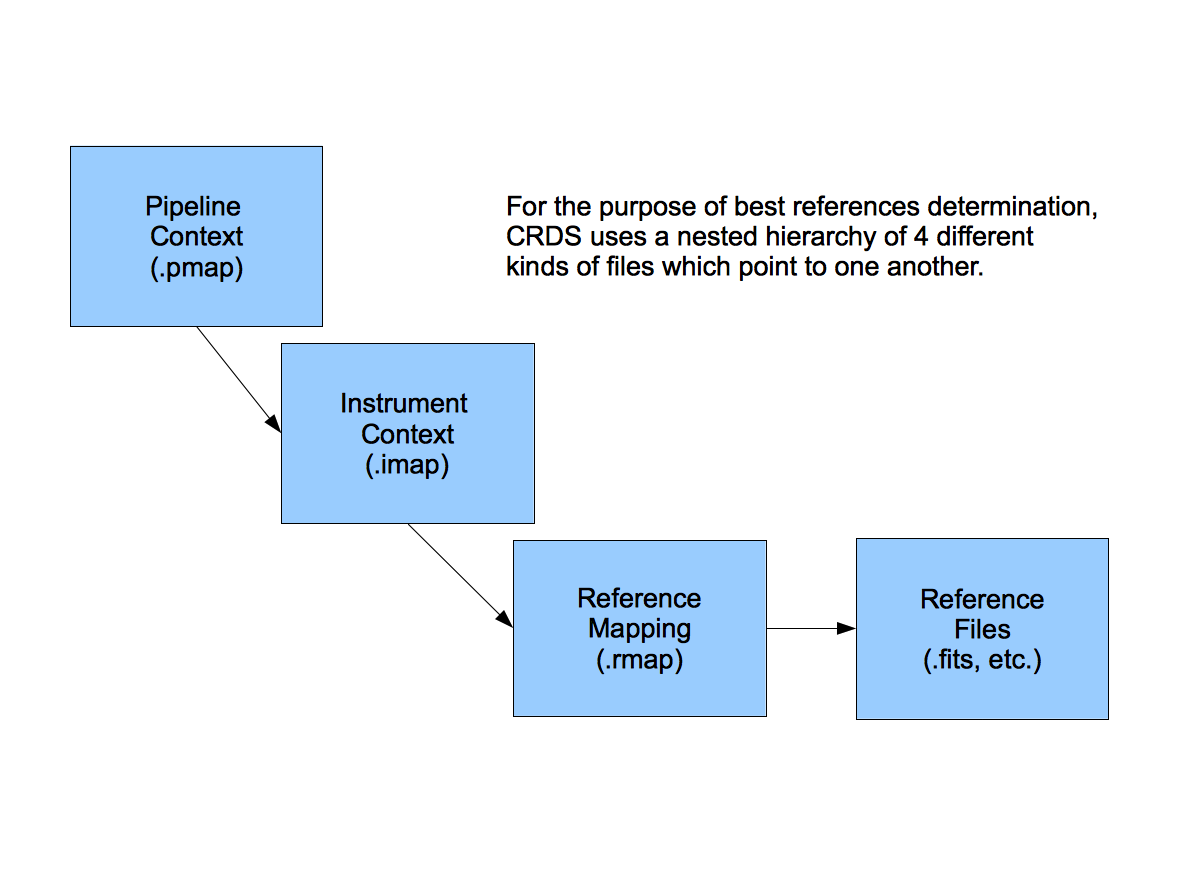
\includegraphics{file_relationships.png}}
\end{figure}


\section{Naming}
\label{rmap_syntax:naming}
The CRDS HST mapping prototypes which are generated from information scraped from
the CDBS web site are named with the forms:

\begin{Verbatim}[commandchars=\\\{\}]
\PYGZlt{}observatory\PYGZgt{} .pmap                               e.g. hst.pmap
\PYGZlt{}observatory\PYGZgt{} \PYGZus{} \PYGZlt{}instrument\PYGZgt{} .imap                e.g. hst\PYGZus{}acs.imap
\PYGZlt{}observatory\PYGZgt{} \PYGZus{} \PYGZlt{}instrument\PYGZgt{} \PYGZus{} \PYGZlt{}filekind\PYGZgt{} .rmap   e.g. hst\PYGZus{}acs\PYGZus{}darkfile.rmap
\end{Verbatim}

The names of subsequent derived mappings include a version number:

\begin{Verbatim}[commandchars=\\\{\}]
\PYGZlt{}observatory\PYGZgt{} \PYGZus{} \PYGZlt{}version\PYGZgt{} .pmap                               e.g. hst\PYGZus{}00001.pmap
\PYGZlt{}observatory\PYGZgt{} \PYGZus{} \PYGZlt{}instrument\PYGZgt{} \PYGZus{} \PYGZlt{}version\PYGZgt{} .imap                e.g. hst\PYGZus{}acs\PYGZus{}00047.imap
\PYGZlt{}observatory\PYGZgt{} \PYGZus{} \PYGZlt{}instrument\PYGZgt{} \PYGZus{} \PYGZlt{}filekind\PYGZgt{} \PYGZus{} \PYGZlt{}version\PYGZgt{} .rmap   e.g. hst\PYGZus{}acs\PYGZus{}darkfile\PYGZus{}00012.rmap
\end{Verbatim}


\section{Basic Structure}
\label{rmap_syntax:basic-structure}
All mappings have the same basic structure consisting of a ``header'' section followe by a ``selector'' section.


\subsection{header}
\label{rmap_syntax:header}
The header provides meta data describing the mapping.  A critical field in the mapping header is the ``parkey''
field which names the dataset parameters (nominally FITS keywords or JWST data model names) which are used by
the selector to do a best references lookup.


\subsection{selector}
\label{rmap_syntax:selector}
The selector provides matching rules used to look up the results of the mapping.  The selector is a nested tree
structure consisting of top-level selectors and sub-selectors.


\section{Pipeline Mappings (.pmap)}
\label{rmap_syntax:pipeline-mappings-pmap}
A sample pipeline mapping for HST looks like:

\begin{Verbatim}[commandchars=\\\{\}]
\PYG{n}{header} \PYG{o}{=} \PYG{p}{\PYGZob{}}
    \PYG{l+s}{\PYGZsq{}}\PYG{l+s}{name}\PYG{l+s}{\PYGZsq{}} \PYG{p}{:} \PYG{l+s}{\PYGZsq{}}\PYG{l+s}{hst.pmap}\PYG{l+s}{\PYGZsq{}}\PYG{p}{,}
    \PYG{l+s}{\PYGZsq{}}\PYG{l+s}{derived\PYGZus{}from}\PYG{l+s}{\PYGZsq{}} \PYG{p}{:} \PYG{l+s}{\PYGZsq{}}\PYG{l+s}{created by hand 12\PYGZhy{}23\PYGZhy{}2011}\PYG{l+s}{\PYGZsq{}}\PYG{p}{,}
    \PYG{l+s}{\PYGZsq{}}\PYG{l+s}{mapping}\PYG{l+s}{\PYGZsq{}} \PYG{p}{:} \PYG{l+s}{\PYGZsq{}}\PYG{l+s}{PIPELINE}\PYG{l+s}{\PYGZsq{}}\PYG{p}{,}
    \PYG{l+s}{\PYGZsq{}}\PYG{l+s}{observatory}\PYG{l+s}{\PYGZsq{}} \PYG{p}{:} \PYG{l+s}{\PYGZsq{}}\PYG{l+s}{HST}\PYG{l+s}{\PYGZsq{}}\PYG{p}{,}
    \PYG{l+s}{\PYGZsq{}}\PYG{l+s}{parkey}\PYG{l+s}{\PYGZsq{}} \PYG{p}{:} \PYG{p}{(}\PYG{l+s}{\PYGZsq{}}\PYG{l+s}{INSTRUME}\PYG{l+s}{\PYGZsq{}}\PYG{p}{,}\PYG{p}{)}\PYG{p}{,}
    \PYG{l+s}{\PYGZsq{}}\PYG{l+s}{description}\PYG{l+s}{\PYGZsq{}} \PYG{p}{:} \PYG{l+s}{\PYGZsq{}}\PYG{l+s}{Initially generated on 12\PYGZhy{}23\PYGZhy{}2011}\PYG{l+s}{\PYGZsq{}}\PYG{p}{,}
    \PYG{l+s}{\PYGZsq{}}\PYG{l+s}{sha1sum}\PYG{l+s}{\PYGZsq{}} \PYG{p}{:} \PYG{l+s}{\PYGZsq{}}\PYG{l+s}{e2c6392fd2731df1e8d933bd990f3fd313a813db}\PYG{l+s}{\PYGZsq{}}\PYG{p}{,}
\PYG{p}{\PYGZcb{}}

\PYG{n}{selector} \PYG{o}{=} \PYG{p}{\PYGZob{}}
    \PYG{l+s}{\PYGZsq{}}\PYG{l+s}{ACS}\PYG{l+s}{\PYGZsq{}} \PYG{p}{:} \PYG{l+s}{\PYGZsq{}}\PYG{l+s}{hst\PYGZus{}acs.imap}\PYG{l+s}{\PYGZsq{}}\PYG{p}{,}
    \PYG{l+s}{\PYGZsq{}}\PYG{l+s}{COS}\PYG{l+s}{\PYGZsq{}} \PYG{p}{:} \PYG{l+s}{\PYGZsq{}}\PYG{l+s}{hst\PYGZus{}cos.imap}\PYG{l+s}{\PYGZsq{}}\PYG{p}{,}
    \PYG{l+s}{\PYGZsq{}}\PYG{l+s}{NICMOS}\PYG{l+s}{\PYGZsq{}} \PYG{p}{:} \PYG{l+s}{\PYGZsq{}}\PYG{l+s}{hst\PYGZus{}nicmos.imap}\PYG{l+s}{\PYGZsq{}}\PYG{p}{,}
    \PYG{l+s}{\PYGZsq{}}\PYG{l+s}{STIS}\PYG{l+s}{\PYGZsq{}} \PYG{p}{:} \PYG{l+s}{\PYGZsq{}}\PYG{l+s}{hst\PYGZus{}stis.imap}\PYG{l+s}{\PYGZsq{}}\PYG{p}{,}
    \PYG{l+s}{\PYGZsq{}}\PYG{l+s}{WFC3}\PYG{l+s}{\PYGZsq{}} \PYG{p}{:} \PYG{l+s}{\PYGZsq{}}\PYG{l+s}{hst\PYGZus{}wfc3.imap}\PYG{l+s}{\PYGZsq{}}\PYG{p}{,}
    \PYG{l+s}{\PYGZsq{}}\PYG{l+s}{WFPC2}\PYG{l+s}{\PYGZsq{}} \PYG{p}{:} \PYG{l+s}{\PYGZsq{}}\PYG{l+s}{hst\PYGZus{}wfpc2.imap}\PYG{l+s}{\PYGZsq{}}\PYG{p}{,}
\PYG{p}{\PYGZcb{}}
\end{Verbatim}

A pipeline mapping matches the dataset ``INSTRUME'' header keyword against its selector to look up an instrument
mapping file.


\section{Instrument Mappings (.imap)}
\label{rmap_syntax:instrument-mappings-imap}
A sample instrument mapping for HST's COS instrument looks like:

\begin{Verbatim}[commandchars=\\\{\}]
\PYG{n}{header} \PYG{o}{=} \PYG{p}{\PYGZob{}}
    \PYG{l+s}{\PYGZsq{}}\PYG{l+s}{derived\PYGZus{}from}\PYG{l+s}{\PYGZsq{}} \PYG{p}{:} \PYG{l+s}{\PYGZsq{}}\PYG{l+s}{scraped 2011\PYGZhy{}12\PYGZhy{}23 11:57:10}\PYG{l+s}{\PYGZsq{}}\PYG{p}{,}
    \PYG{l+s}{\PYGZsq{}}\PYG{l+s}{description}\PYG{l+s}{\PYGZsq{}} \PYG{p}{:} \PYG{l+s}{\PYGZsq{}}\PYG{l+s}{Initially generated on 2011\PYGZhy{}12\PYGZhy{}23 11:57:10}\PYG{l+s}{\PYGZsq{}}\PYG{p}{,}
    \PYG{l+s}{\PYGZsq{}}\PYG{l+s}{instrument}\PYG{l+s}{\PYGZsq{}} \PYG{p}{:} \PYG{l+s}{\PYGZsq{}}\PYG{l+s}{COS}\PYG{l+s}{\PYGZsq{}}\PYG{p}{,}
    \PYG{l+s}{\PYGZsq{}}\PYG{l+s}{mapping}\PYG{l+s}{\PYGZsq{}} \PYG{p}{:} \PYG{l+s}{\PYGZsq{}}\PYG{l+s}{INSTRUMENT}\PYG{l+s}{\PYGZsq{}}\PYG{p}{,}
    \PYG{l+s}{\PYGZsq{}}\PYG{l+s}{name}\PYG{l+s}{\PYGZsq{}} \PYG{p}{:} \PYG{l+s}{\PYGZsq{}}\PYG{l+s}{hst\PYGZus{}cos.imap}\PYG{l+s}{\PYGZsq{}}\PYG{p}{,}
    \PYG{l+s}{\PYGZsq{}}\PYG{l+s}{observatory}\PYG{l+s}{\PYGZsq{}} \PYG{p}{:} \PYG{l+s}{\PYGZsq{}}\PYG{l+s}{HST}\PYG{l+s}{\PYGZsq{}}\PYG{p}{,}
    \PYG{l+s}{\PYGZsq{}}\PYG{l+s}{parkey}\PYG{l+s}{\PYGZsq{}} \PYG{p}{:} \PYG{p}{(}\PYG{l+s}{\PYGZsq{}}\PYG{l+s}{REFTYPE}\PYG{l+s}{\PYGZsq{}}\PYG{p}{,}\PYG{p}{)}\PYG{p}{,}
    \PYG{l+s}{\PYGZsq{}}\PYG{l+s}{sha1sum}\PYG{l+s}{\PYGZsq{}} \PYG{p}{:} \PYG{l+s}{\PYGZsq{}}\PYG{l+s}{800fb1567cb5bed4031402c7396aeb86c5e1db61}\PYG{l+s}{\PYGZsq{}}\PYG{p}{,}
    \PYG{l+s}{\PYGZsq{}}\PYG{l+s}{source\PYGZus{}url}\PYG{l+s}{\PYGZsq{}} \PYG{p}{:} \PYG{l+s}{\PYGZsq{}}\PYG{l+s}{http://www.stsci.edu/hst/observatory/cdbs/SIfileInfo/COS/reftablequeryindex}\PYG{l+s}{\PYGZsq{}}\PYG{p}{,}
\PYG{p}{\PYGZcb{}}

\PYG{n}{selector} \PYG{o}{=} \PYG{p}{\PYGZob{}}
    \PYG{l+s}{\PYGZsq{}}\PYG{l+s}{badttab}\PYG{l+s}{\PYGZsq{}} \PYG{p}{:} \PYG{l+s}{\PYGZsq{}}\PYG{l+s}{hst\PYGZus{}cos\PYGZus{}badttab.rmap}\PYG{l+s}{\PYGZsq{}}\PYG{p}{,}
    \PYG{l+s}{\PYGZsq{}}\PYG{l+s}{bpixtab}\PYG{l+s}{\PYGZsq{}} \PYG{p}{:} \PYG{l+s}{\PYGZsq{}}\PYG{l+s}{hst\PYGZus{}cos\PYGZus{}bpixtab.rmap}\PYG{l+s}{\PYGZsq{}}\PYG{p}{,}
    \PYG{l+s}{\PYGZsq{}}\PYG{l+s}{brftab}\PYG{l+s}{\PYGZsq{}} \PYG{p}{:} \PYG{l+s}{\PYGZsq{}}\PYG{l+s}{hst\PYGZus{}cos\PYGZus{}brftab.rmap}\PYG{l+s}{\PYGZsq{}}\PYG{p}{,}
    \PYG{l+s}{\PYGZsq{}}\PYG{l+s}{brsttab}\PYG{l+s}{\PYGZsq{}} \PYG{p}{:} \PYG{l+s}{\PYGZsq{}}\PYG{l+s}{hst\PYGZus{}cos\PYGZus{}brsttab.rmap}\PYG{l+s}{\PYGZsq{}}\PYG{p}{,}
    \PYG{l+s}{\PYGZsq{}}\PYG{l+s}{deadtab}\PYG{l+s}{\PYGZsq{}} \PYG{p}{:} \PYG{l+s}{\PYGZsq{}}\PYG{l+s}{hst\PYGZus{}cos\PYGZus{}deadtab.rmap}\PYG{l+s}{\PYGZsq{}}\PYG{p}{,}
    \PYG{l+s}{\PYGZsq{}}\PYG{l+s}{disptab}\PYG{l+s}{\PYGZsq{}} \PYG{p}{:} \PYG{l+s}{\PYGZsq{}}\PYG{l+s}{hst\PYGZus{}cos\PYGZus{}disptab.rmap}\PYG{l+s}{\PYGZsq{}}\PYG{p}{,}
    \PYG{l+s}{\PYGZsq{}}\PYG{l+s}{flatfile}\PYG{l+s}{\PYGZsq{}} \PYG{p}{:} \PYG{l+s}{\PYGZsq{}}\PYG{l+s}{hst\PYGZus{}cos\PYGZus{}flatfile.rmap}\PYG{l+s}{\PYGZsq{}}\PYG{p}{,}
    \PYG{l+s}{\PYGZsq{}}\PYG{l+s}{fluxtab}\PYG{l+s}{\PYGZsq{}} \PYG{p}{:} \PYG{l+s}{\PYGZsq{}}\PYG{l+s}{hst\PYGZus{}cos\PYGZus{}fluxtab.rmap}\PYG{l+s}{\PYGZsq{}}\PYG{p}{,}
    \PYG{l+s}{\PYGZsq{}}\PYG{l+s}{geofile}\PYG{l+s}{\PYGZsq{}} \PYG{p}{:} \PYG{l+s}{\PYGZsq{}}\PYG{l+s}{hst\PYGZus{}cos\PYGZus{}geofile.rmap}\PYG{l+s}{\PYGZsq{}}\PYG{p}{,}
    \PYG{l+s}{\PYGZsq{}}\PYG{l+s}{lamptab}\PYG{l+s}{\PYGZsq{}} \PYG{p}{:} \PYG{l+s}{\PYGZsq{}}\PYG{l+s}{hst\PYGZus{}cos\PYGZus{}lamptab.rmap}\PYG{l+s}{\PYGZsq{}}\PYG{p}{,}
    \PYG{l+s}{\PYGZsq{}}\PYG{l+s}{phatab}\PYG{l+s}{\PYGZsq{}} \PYG{p}{:} \PYG{l+s}{\PYGZsq{}}\PYG{l+s}{hst\PYGZus{}cos\PYGZus{}phatab.rmap}\PYG{l+s}{\PYGZsq{}}\PYG{p}{,}
    \PYG{l+s}{\PYGZsq{}}\PYG{l+s}{spwcstab}\PYG{l+s}{\PYGZsq{}} \PYG{p}{:} \PYG{l+s}{\PYGZsq{}}\PYG{l+s}{hst\PYGZus{}cos\PYGZus{}spwcstab.rmap}\PYG{l+s}{\PYGZsq{}}\PYG{p}{,}
    \PYG{l+s}{\PYGZsq{}}\PYG{l+s}{tdstab}\PYG{l+s}{\PYGZsq{}} \PYG{p}{:} \PYG{l+s}{\PYGZsq{}}\PYG{l+s}{hst\PYGZus{}cos\PYGZus{}tdstab.rmap}\PYG{l+s}{\PYGZsq{}}\PYG{p}{,}
    \PYG{l+s}{\PYGZsq{}}\PYG{l+s}{wcptab}\PYG{l+s}{\PYGZsq{}} \PYG{p}{:} \PYG{l+s}{\PYGZsq{}}\PYG{l+s}{hst\PYGZus{}cos\PYGZus{}wcptab.rmap}\PYG{l+s}{\PYGZsq{}}\PYG{p}{,}
    \PYG{l+s}{\PYGZsq{}}\PYG{l+s}{xtractab}\PYG{l+s}{\PYGZsq{}} \PYG{p}{:} \PYG{l+s}{\PYGZsq{}}\PYG{l+s}{hst\PYGZus{}cos\PYGZus{}xtractab.rmap}\PYG{l+s}{\PYGZsq{}}\PYG{p}{,}
\PYG{p}{\PYGZcb{}}
\end{Verbatim}

Instrument mappings match the desired reference file type against the reference mapping which can be used to determine a
best reference recommendation for a particular dataset.  An instrument mapping lists all possible reference types for
all modes of the instrument,  some of which may not be appropriate for a particular mode.   The selector key of an
instrument mapping is the value of a reference file header keyword ``REFTYPE'',  and is the name of the dataset header
keyword which will record the best reference selection.


\section{Reference Mappings (.rmap)}
\label{rmap_syntax:reference-mappings-rmap}
A sample reference mapping for HST COS DEADTAB looks like:

\begin{Verbatim}[commandchars=\\\{\}]
\PYG{n}{header} \PYG{o}{=} \PYG{p}{\PYGZob{}}
    \PYG{l+s}{\PYGZsq{}}\PYG{l+s}{derived\PYGZus{}from}\PYG{l+s}{\PYGZsq{}} \PYG{p}{:} \PYG{l+s}{\PYGZsq{}}\PYG{l+s}{scraped 2011\PYGZhy{}12\PYGZhy{}23 11:54:56}\PYG{l+s}{\PYGZsq{}}\PYG{p}{,}
    \PYG{l+s}{\PYGZsq{}}\PYG{l+s}{description}\PYG{l+s}{\PYGZsq{}} \PYG{p}{:} \PYG{l+s}{\PYGZsq{}}\PYG{l+s}{Initially generated on 2011\PYGZhy{}12\PYGZhy{}23 11:54:56}\PYG{l+s}{\PYGZsq{}}\PYG{p}{,}
    \PYG{l+s}{\PYGZsq{}}\PYG{l+s}{filekind}\PYG{l+s}{\PYGZsq{}} \PYG{p}{:} \PYG{l+s}{\PYGZsq{}}\PYG{l+s}{DEADTAB}\PYG{l+s}{\PYGZsq{}}\PYG{p}{,}
    \PYG{l+s}{\PYGZsq{}}\PYG{l+s}{instrument}\PYG{l+s}{\PYGZsq{}} \PYG{p}{:} \PYG{l+s}{\PYGZsq{}}\PYG{l+s}{COS}\PYG{l+s}{\PYGZsq{}}\PYG{p}{,}
    \PYG{l+s}{\PYGZsq{}}\PYG{l+s}{mapping}\PYG{l+s}{\PYGZsq{}} \PYG{p}{:} \PYG{l+s}{\PYGZsq{}}\PYG{l+s}{REFERENCE}\PYG{l+s}{\PYGZsq{}}\PYG{p}{,}
    \PYG{l+s}{\PYGZsq{}}\PYG{l+s}{name}\PYG{l+s}{\PYGZsq{}} \PYG{p}{:} \PYG{l+s}{\PYGZsq{}}\PYG{l+s}{hst\PYGZus{}cos\PYGZus{}deadtab.rmap}\PYG{l+s}{\PYGZsq{}}\PYG{p}{,}
    \PYG{l+s}{\PYGZsq{}}\PYG{l+s}{observatory}\PYG{l+s}{\PYGZsq{}} \PYG{p}{:} \PYG{l+s}{\PYGZsq{}}\PYG{l+s}{HST}\PYG{l+s}{\PYGZsq{}}\PYG{p}{,}
    \PYG{l+s}{\PYGZsq{}}\PYG{l+s}{parkey}\PYG{l+s}{\PYGZsq{}} \PYG{p}{:} \PYG{p}{(}\PYG{p}{(}\PYG{l+s}{\PYGZsq{}}\PYG{l+s}{DETECTOR}\PYG{l+s}{\PYGZsq{}}\PYG{p}{,}\PYG{p}{)}\PYG{p}{,} \PYG{p}{(}\PYG{l+s}{\PYGZsq{}}\PYG{l+s}{DATE\PYGZhy{}OBS}\PYG{l+s}{\PYGZsq{}}\PYG{p}{,} \PYG{l+s}{\PYGZsq{}}\PYG{l+s}{TIME\PYGZhy{}OBS}\PYG{l+s}{\PYGZsq{}}\PYG{p}{)}\PYG{p}{)}\PYG{p}{,}
    \PYG{l+s}{\PYGZsq{}}\PYG{l+s}{sha1sum}\PYG{l+s}{\PYGZsq{}} \PYG{p}{:} \PYG{l+s}{\PYGZsq{}}\PYG{l+s}{e27984a6441d8aaa7cd28ead2267a6be4c3a153b}\PYG{l+s}{\PYGZsq{}}\PYG{p}{,}
\PYG{p}{\PYGZcb{}}

\PYG{n}{selector} \PYG{o}{=} \PYG{n}{Match}\PYG{p}{(}\PYG{p}{\PYGZob{}}
    \PYG{p}{(}\PYG{l+s}{\PYGZsq{}}\PYG{l+s}{FUV}\PYG{l+s}{\PYGZsq{}}\PYG{p}{,}\PYG{p}{)} \PYG{p}{:} \PYG{n}{UseAfter}\PYG{p}{(}\PYG{p}{\PYGZob{}}
        \PYG{l+s}{\PYGZsq{}}\PYG{l+s}{1996\PYGZhy{}10\PYGZhy{}01 00:00:00}\PYG{l+s}{\PYGZsq{}} \PYG{p}{:} \PYG{l+s}{\PYGZsq{}}\PYG{l+s}{s7g1700gl\PYGZus{}dead.fits}\PYG{l+s}{\PYGZsq{}}\PYG{p}{,}
    \PYG{p}{\PYGZcb{}}\PYG{p}{)}\PYG{p}{,}
    \PYG{p}{(}\PYG{l+s}{\PYGZsq{}}\PYG{l+s}{NUV}\PYG{l+s}{\PYGZsq{}}\PYG{p}{,}\PYG{p}{)} \PYG{p}{:} \PYG{n}{UseAfter}\PYG{p}{(}\PYG{p}{\PYGZob{}}
        \PYG{l+s}{\PYGZsq{}}\PYG{l+s}{1996\PYGZhy{}10\PYGZhy{}01 00:00:00}\PYG{l+s}{\PYGZsq{}} \PYG{p}{:} \PYG{l+s}{\PYGZsq{}}\PYG{l+s}{s7g1700ql\PYGZus{}dead.fits}\PYG{l+s}{\PYGZsq{}}\PYG{p}{,}
    \PYG{p}{\PYGZcb{}}\PYG{p}{)}\PYG{p}{,}
\PYG{p}{\PYGZcb{}}\PYG{p}{)}
\end{Verbatim}

Reference mapping selectors are constructed as a nested hierarchy of selection operators which match against
various dataset header keywords.


\section{Active Header Fields}
\label{rmap_syntax:active-header-fields}
Many rmap header fields are passive metadata.   A number of optional rmap header fields,  however,  actively affect
best reference lookups and results:

\begin{Verbatim}[commandchars=\\\{\}]
header = \PYGZob{}
          ...,

    \PYGZsq{}parkey\PYGZsq{} : ((\PYGZsq{}DETECTOR\PYGZsq{},), (\PYGZsq{}DATE\PYGZhy{}OBS\PYGZsq{}, \PYGZsq{}TIME\PYGZhy{}OBS\PYGZsq{})),

    \PYGZsq{}extra\PYGZus{}keys\PYGZsq{} : (\PYGZsq{}XCORNER\PYGZsq{}, \PYGZsq{}YCORNER\PYGZsq{}, \PYGZsq{}CCDCHIP\PYGZsq{}),

    \PYGZsq{}reffile\PYGZus{}switch\PYGZsq{} : \PYGZsq{}BIASCORR\PYGZsq{},

    \PYGZsq{}reffile\PYGZus{}required\PYGZsq{} : \PYGZsq{}YES\PYGZsq{},

    \PYGZsq{}rmap\PYGZus{}relevance\PYGZsq{} : \PYGZsq{}((DETECTOR != \PYGZdq{}SBC\PYGZdq{}) and (BIASCORR != \PYGZdq{}OMIT\PYGZdq{}))\PYGZsq{},
    \PYGZsq{}rmap\PYGZus{}omit\PYGZsq{} : \PYGZsq{}((DETECTOR != \PYGZdq{}SBC\PYGZdq{}) and (BIASCORR != \PYGZdq{}OMIT\PYGZdq{}))\PYGZsq{},

    \PYGZsq{}parkey\PYGZus{}relevance\PYGZsq{} : \PYGZob{}
        \PYGZsq{}binaxis1\PYGZsq{} : \PYGZsq{}(DETECTOR == \PYGZdq{}UVIS\PYGZdq{})\PYGZsq{},
        \PYGZsq{}binaxis2\PYGZsq{} : \PYGZsq{}(DETECTOR == \PYGZdq{}UVIS\PYGZdq{})\PYGZsq{},
        \PYGZsq{}ccdgain\PYGZsq{} : \PYGZsq{}(DETECTOR == \PYGZdq{}IR\PYGZdq{})\PYGZsq{},
        \PYGZsq{}samp\PYGZus{}seq\PYGZsq{} : \PYGZsq{}(DETECTOR == \PYGZdq{}IR\PYGZdq{})\PYGZsq{},
        \PYGZsq{}subtype\PYGZsq{} : \PYGZsq{}(DETECTOR == \PYGZdq{}IR\PYGZdq{})\PYGZsq{},
    \PYGZcb{},

    \PYGZsq{}hooks\PYGZsq{} : \PYGZob{}
        \PYGZsq{}fallback\PYGZus{}header\PYGZsq{} : \PYGZsq{}fallback\PYGZus{}header\PYGZus{}acs\PYGZus{}biasfile\PYGZus{}v2\PYGZsq{},
        \PYGZsq{}precondition\PYGZus{}header\PYGZsq{} : \PYGZsq{}precondition\PYGZus{}header\PYGZus{}acs\PYGZus{}biasfile\PYGZus{}v2\PYGZsq{},
    \PYGZcb{},

          ...,
\PYGZcb{}
\end{Verbatim}


\subsection{Required Parameters}
\label{rmap_syntax:required-parameters}
Required matching parameters for computing best references are defined by the union of 3 header fields:  \emph{parkey},
\emph{extra\_keys}, and  \emph{reffile\_switch}.   There is no requirement to use all 3 forms,  the latter two forms were added
to model and emulate aspects of HST's CDBS system,  the precursor to CRDS.


\subsubsection{parkey}
\label{rmap_syntax:parkey}
The primary location for defining best references matching parameters is the \emph{parkey} field.

The simplest form of \emph{parkey} is a tuple of parameter names used in a lookup by a non-nested selector,  as is
seen in pipeline and instrument mappings above.

In reference mappings,  the header \emph{parkey} field is a tuple of tuples.  Each stage of the nested selector
consumes the next tuple of header keys.  The same parameter set and matching structure is shared by all sections
of a single rmap.   For mode-specific parameters,  two approaches are availble:  use a separate .rmap for each
parameter combination, or fill in unused parameters for a particular mode with the value `N/A'.

For the HST COS DEADTAB example above,   the Match operator matches against the value of the dataset keyword
`DETECTOR'.   Based on that match, the selected UseAfter operator matches against the dataset's `DATE-OBS' and
`TIME-OBS' keywords to lookup the name of a reference file.

There is no default for parkey.


\subsubsection{extra\_keys}
\label{rmap_syntax:extra-keys}
\emph{extra\_keys} specifies a tuple of parameter names which will not be used in the matches directly,  but may be used by
rmap header expressions and hook functions to influence matching.  Listing parameters in extra\_keys ensures that the
CRDS infrastructure will request the parameters from the server or dataset files and make them available during best
references computations and logical expression evaluation.   All parameters used in logical expressions must be
explicitly defined and listed.   Undefined parameters are evaluated with the value `UNDEFINED'.

If omitted, \emph{extra\_keys} defaults to (),  no extra keys.


\subsubsection{reffile\_switch}
\label{rmap_syntax:reffile-switch}
Nominally names a dataset keyword generally of the form \textless{}type\textgreater{}CORR with keyword values `PERFORM' and `OMIT'.

If \emph{reffile\_switch} is not `NONE',  it specifies an extra keyword value is to fetch from the dataset.

If \emph{reffile\_switch} is omitted or `NONE',  no keyword value is fetched from the dataset.

The runtime checking \emph{reffile\_switch} is used for must be explicitly implemented as part of an \emph{rmap\_relevance} or
\emph{rmap\_omit} expression as seen in the example header; \emph{reffile\_switch} only specifies an extra parameter to fetch
for use in logical expressions and matching.  It is logically equivalent to adding the parameter to \emph{extra\_keys}.


\subsection{Logical Header Expressions}
\label{rmap_syntax:logical-header-expressions}
A number of the subsequently described features employ logical expressions which are evaluated at match-time
based on the values in the dataset header.  There are several things to point out:
\begin{itemize}
\item {} 
Logical expressions are evaluated in the context of the required parameters discussed above.

\item {} 
Dataset matching parameters appear in logical expressions in upper case,  without quotes, like global variables.

\item {} 
The entire expression is enclosed in parentheses to tell CRDS to leave case as-is.

\item {} 
Logical expressions are limited to a restricted subset of Python expressions,  not arbitrary Python.  In particular
arbitrary Python function calls are not permitted.

\end{itemize}


\subsection{reffile\_required}
\label{rmap_syntax:reffile-required}
Defines what should happen if an rmap lookup cannot find a match for a particular reference type.

\emph{reffile\_required} has legal values `YES', `NO', and `NONE'.

If \emph{reffile\_required} is `YES', failing to find a match results in an exception and/or ERROR.

If \emph{reffile\_required} is `NONE', CDBS did not define \emph{reffile\_required} for this type, so it is assumed to be required.

If \emph{reffile\_required} is `NO',  failing to find a match results in assigning the value `N/A' rather than failing.


\subsection{rmap\_relevance}
\label{rmap_syntax:rmap-relevance}
\emph{rmap\_relevance} is a logical expression which is evaluated in the context of dataset header variables.

If \emph{rmap\_relevance} evaluates to True, then a full match is performed and the resulting bestref is returned.

If \emph{rmap\_relevance} evaluates to False, then the match is short circuited and `N/A' is assigned.


\subsection{parkey\_relevance}
\label{rmap_syntax:parkey-relevance}
\emph{parkey\_relevance} defines a mapping from dataset matching parameters to logical expressions.

\emph{parkey\_relevance} is evaluated in the context of the entire set of matching parameters and mutates
the specified parameter to `N/A' if the expression evaluates to False,  i.e. the parameter is not relevant
in the context of the other parameter values.

When a parameter value of `N/A' is used for matching, the parameter is effectively ignored.


\subsection{hooks}
\label{rmap_syntax:hooks}
The \emph{hooks} header section defines functions which are used for special case processing for complex reference
assignments.   The existing hooks were devised to emulate similar special case handling performed by CRDS's
predecessor system CDBS.

The original \textless{}100 series of HST rules had implicit hooks.  CRDS rules \textgreater{}200 have hooks which are explicitly
named in the `hooks' section of the header which indicates that customized matching is being performed.   Running
crds.bestrefs with --verbosity=60 wil issue log messages describing hook operations.

new hook functions can only be added with a new release of CRDS code.   hook functions have versioned names and should
never be modified after use in operations since that would change the meaning of historical .rmaps.  Instead,  a new
hook function should be added and the .rmap header modified to assign it.

hook functions can be `unplugged' in an operational .rmap by setting the value of the hook to `none'.  Removing the
`hooks' section of the .rmap header, or removing individual hook names, currently results in reversion to \textless{}100 series
.rmap behavior and the original implicit hook functions.


\subsubsection{precondition\_header}
\label{rmap_syntax:precondition-header}
The \emph{precondition\_header} hook is used to mutate incoming dataset matching parameters.   \emph{precondition\_header} is
sometimes justified as reductive,  written in terms of \emph{extra\_parkeys} which do not appear in the matching tuples,
and used to mutate a broad range of matching parameter values onto a narrower set of parameter values known to be
handled in the .rmap.   In essence,  when a \emph{precondition\_header} hook is used,  the dataset matching parameters
become a function of themselves.


\subsubsection{fallback\_header}
\label{rmap_syntax:fallback-header}
The \emph{fallback\_header} hook is used to mutate incoming dataset matching parameters similar to \emph{precondition\_header}.
The \emph{fallback\_header} hook is called when the first matching attempt for dataset parameters fails.  \emph{fallback\_header}
computes a set of matching parameters used for a second matching attempt which will return normally if succesful.


\section{Selectors}
\label{rmap_syntax:selectors}
All the CRDS selection operators are written to select either a return
value \emph{or} a nested operator.  In the case of HST, the Match operator locates a
nested UseAfter operator which in turn locates the reference file.


\subsection{Primitive Return Values}
\label{rmap_syntax:primitive-return-values}
Ultimately the result of every selector lookup is some form of return value to
which various CRDS operations can be applied: best references assignment, file
distribution, file certification, file differencing, etc.


\subsubsection{Single Filename}
\label{rmap_syntax:single-filename}
The most typical return value is a single reference filename.  In the case of
GEIS files, for the data+header file pair the header is specified in rmaps but
both components are distributed.


\subsubsection{Filename Tuple}
\label{rmap_syntax:filename-tuple}
A tuple of primitive filenames can be specified.  All files in the tuple are
synchronized and returned as best references.  The nominal application of a
file tuple is for the bracket selector where the files are used for pipeline
side interpolations between the two references to generate a synthetic
reference.


\subsubsection{Not Applicable}
\label{rmap_syntax:not-applicable}
A value of N/A can be assigned in place of a filename.  This applies the full
power of the matching system to the specification of instrument modes for which
a reference type does not apply.  For JWST this feature is used to perform data
driven WCS processing based on CRDS reference file assignments.  Ultimately the
best reference assigned is N/A, nominally explicitly recorded for the type
keyword.  No file is distributed or prefetched.  N/A may be specified in place
of a reference file or an rmap file.  In the case of specifying N/A for an rmap
file (in the imap/instrument mapping), that type becomes N/A for all modes of
that instrument.


\subsubsection{Omit}
\label{rmap_syntax:omit}
Similar to N/A, a value of OMIT can be specified in place of a filename.  OMIT
can be used to completely remove a type from the best references response.  No
file is synchronized or processed, and no best reference should be recorded in
the dataset header for that type.  This feature is currently unused.


\subsection{Match}
\label{rmap_syntax:match}
Based on a dataset{}`s header values,  Match locates the match tuple which best matches the dataset.   Conceptually this
is a dictionary lookup.   In actuality, CRDS processes each match parameter in succession,  at each step eliminating
match candidates that cannot possibly match.


\subsubsection{Parameter Tuples and Simple Matches}
\label{rmap_syntax:parameter-tuples-and-simple-matches}
The CRDS Match operator typically matches a dataset header against a tuple which defines multiple parameter values whose
names are specified in the rmap header \code{parkey}:

\begin{Verbatim}[commandchars=\\\{\}]
(\PYGZdq{}UVIS\PYGZdq{}, \PYGZdq{}F122LP\PYGZdq{})   :  \PYGZsq{}some\PYGZus{}file\PYGZus{}or\PYGZus{}nested\PYGZus{}selection\PYGZsq{}
\end{Verbatim}

Alternately,  for simple use cases the Match operator can match against single
strings,  which is a simplified syntax for a 1-tuple:

\begin{Verbatim}[commandchars=\\\{\}]
\PYGZsq{}UVIS\PYGZsq{}  :  \PYGZsq{}some\PYGZus{}file\PYGZus{}or\PYGZus{}nested\PYGZus{}selection\PYGZsq{}
(\PYGZsq{}UVIS\PYGZsq{},) : \PYGZsq{}this\PYGZus{}is\PYGZus{}the\PYGZus{}equivalent\PYGZus{}one\PYGZus{}tuple\PYGZsq{}
\end{Verbatim}


\subsubsection{Single Parameter Values}
\label{rmap_syntax:single-parameter-values}
Each value within the match tuples of a Match operator can be an expression in its own right.   There are a number of
special values associated with each match expression:  Ors \textbar{}, Wildcards *,  Regular Expressions (), Literals \{\},
Relationals, between, N/A, and Substitutions.


\subsubsection{Or \textbar{}}
\label{rmap_syntax:or}
Many CRDS match expressions consist of a series of match patterns separated by vertical bars.   The vertical bar is read
as ``or'' and means that a match occurs if either pattern matches that dataset header.   For example, the expression:

\begin{Verbatim}[commandchars=\\\{\}]
(\PYGZdq{}either\PYGZus{}this\textbar{}that\PYGZdq{},\PYGZdq{}1\textbar{}2\textbar{}3\PYGZdq{})  : \PYGZdq{}some\PYGZus{}file.fits\PYGZdq{}
\end{Verbatim}

will match:

\begin{Verbatim}[commandchars=\\\{\}]
\PYG{p}{(}\PYG{l+s}{\PYGZdq{}}\PYG{l+s}{either\PYGZus{}this}\PYG{l+s}{\PYGZdq{}}\PYG{p}{,} \PYG{l+s}{\PYGZdq{}}\PYG{l+s}{2}\PYG{l+s}{\PYGZdq{}}\PYG{p}{)}
\end{Verbatim}

and also:

\begin{Verbatim}[commandchars=\\\{\}]
\PYG{p}{(}\PYG{l+s}{\PYGZdq{}}\PYG{l+s}{that}\PYG{l+s}{\PYGZdq{}}\PYG{p}{,} \PYG{l+s}{\PYGZdq{}}\PYG{l+s}{1}\PYG{l+s}{\PYGZdq{}}\PYG{p}{)}
\end{Verbatim}


\subsubsection{Wild Cards *}
\label{rmap_syntax:wild-cards}
By default,  * is interpreted in CRDS as a glob pattern,  much like UNIX shell file name matching.  * matches any
sequence of characters.  The expression:

\begin{Verbatim}[commandchars=\\\{\}]
(\PYGZdq{}F*122\PYGZdq{},) : \PYGZdq{}some\PYGZus{}file.fits\PYGZdq{}
\end{Verbatim}

will match any value starting with ``F'' and ending with ``122''.


\subsubsection{Regular Expressions}
\label{rmap_syntax:regular-expressions}
CRDS can match on true regular expressions.   A true regular expression match is
triggered by bracketing the match in parentheses ():

\begin{Verbatim}[commandchars=\\\{\}]
(\PYGZdq{}(\PYGZca{}F[\PYGZca{}13]22\PYGZdl{})\PYGZdq{},)  : \PYGZdq{}some\PYGZus{}file.fits\PYGZdq{}
\end{Verbatim}

The above corresponds to matching the regular expression ``\textasciicircum{}F{[}\textasciicircum{}1234{]}22\$'' (note that the bracketing parentheses within the
string are removed.)   Regular expression syntax is explained in the Python documentation for the re module. The above
expression will match values starting with ``F'', followed by any character which is not ``1'' or ``3'' followed by ``22''.


\subsubsection{Literal Expressions}
\label{rmap_syntax:literal-expressions}
A literal expression is bracketed with curly braces \{\} and is matched without
any interpretation whatsoever.   Hence,  special characters like * or \textbar{} are
interpreted literally rather than as ors or wildcards.  The expression:

\begin{Verbatim}[commandchars=\\\{\}]
(\PYGZdq{}\PYGZob{}F\textbar{}*G\PYGZcb{}\PYGZdq{},) : \PYGZdq{}some\PYGZus{}file.fits\PYGZdq{}
\end{Verbatim}

matches the value ``F\textbar{}*G'' as opposed to ``F'' or anything ending with ``G''.


\subsubsection{Relational Expressions}
\label{rmap_syntax:relational-expressions}
Relational expressions are bracketed by the pound character \#.   Relational
expressions do numerical comparisons on the header value to determine a match.
Relational expressions have implicit variables and support the operators:

\begin{Verbatim}[commandchars=\\\{\}]
\PYGZgt{} \PYGZgt{}= \PYGZlt{} \PYGZlt{}= == and or
\end{Verbatim}

The expression:

\begin{Verbatim}[commandchars=\\\{\}]
(\PYGZdq{}\PYGZsh{} \PYGZgt{}1 and \PYGZlt{}37 \PYGZsh{}\PYGZdq{},)  : \PYGZdq{}some\PYGZus{}file.fits\PYGZdq{}
\end{Verbatim}

will match any number greater than 1 and less than 37.


\subsubsection{Between}
\label{rmap_syntax:between}
A special relational operator ``between'' is used to simply express a range
of numbers \textgreater{}= to the lower bound and \textless{} the upper bound,  similar to Python
slicing:

\begin{Verbatim}[commandchars=\\\{\}]
(\PYGZdq{}between 1  47\PYGZdq{},) : \PYGZdq{}some\PYGZus{}file.fits\PYGZdq{}
\end{Verbatim}

will match any number greater than or equal to 1 and less than 47.   This is
equivalent to:

\begin{Verbatim}[commandchars=\\\{\}]
(\PYGZdq{}\PYGZsh{} \PYGZgt{}=1 and \PYGZlt{}47 \PYGZsh{}\PYGZdq{},) : \PYGZdq{}some\PYGZus{}file.fits\PYGZdq{}
\end{Verbatim}

Note that ``between'' matches sensibly stack into a complete range.  The expressions:

\begin{Verbatim}[commandchars=\\\{\}]
(\PYGZdq{}between 1 47\PYGZdq{},) : \PYGZdq{}some\PYGZus{}file.fits\PYGZdq{}
(\PYGZdq{}between 47 90\PYGZdq{}, ) : \PYGZdq{}another\PYGZus{}file.fits\PYGZdq{}
\end{Verbatim}

provide complete coverage for the range between 1 and 90.


\subsubsection{N/A}
\label{rmap_syntax:n-a}
Some rmaps have match tuple values of ``N/A'',  or Not Applicable.
A value of N/A is matched as a special version of ``*'', matching anything,  but
not affecting the ``weight'' of the match:

\begin{Verbatim}[commandchars=\\\{\}]
(\PYGZsq{}HRC\PYGZsq{}, \PYGZsq{}N/A\PYGZsq{}) :  \PYGZdq{}some\PYGZus{}file.fits\PYGZdq{}
\end{Verbatim}

There are a couple uses for N/A parameters.    First,  sometimes a parameter is
irrelevant in the context of the other parameters.   So for an rmap which covers
multiple instrument modes,  a parameter may not apply to all modes. Second,
sometimes a parameter is relevant to custom lookup code,  but is not used by the
match directly.  In this second case,   the ``N/A'' parameter may be used by custom
header preconditioning code to assist in mutating the other parameter values
that \emph{are} used in the match.


\subsubsection{NOT Expressions}
\label{rmap_syntax:not-expressions}
It's possible to match the negation of match expressions by pre-pending ``NOT ''
to the unnegated expression.   For example:

\begin{Verbatim}[commandchars=\\\{\}]
(\PYGZsq{}not HRC\PYGZsq{}, \PYGZsq{}N/A\PYGZsq{}) :  \PYGZdq{}not\PYGZus{}some\PYGZus{}file.fits\PYGZdq{}
\end{Verbatim}

The weight of a negated expression is the opposite of unnegated weight of the
expression: -1 -\textgreater{} 1, 1 -\textgreater{} -1, 0 -\textgreater{} 0.


\subsubsection{Substitution Parameters}
\label{rmap_syntax:substitution-parameters}
Substituion parameters are short hand notation which eliminate the need to
duplicate rmap rules.  In order to support WFC3 biasfile conventions,  CRDS
rmaps permit the definition of meta-match-values which correspond to a set of
actual dataset header values. For instance,  when an rmap header contains a
``substitutions'' field like this:

\begin{Verbatim}[commandchars=\\\{\}]
\PYGZsq{}substitutions\PYGZsq{} : \PYGZob{}
    \PYGZsq{}CCDAMP\PYGZsq{} : \PYGZob{}
        \PYGZsq{}G280\PYGZus{}AMPS\PYGZsq{} : (\PYGZsq{}ABCD\PYGZsq{}, \PYGZsq{}A\PYGZsq{}, \PYGZsq{}B\PYGZsq{}, \PYGZsq{}C\PYGZsq{}, \PYGZsq{}D\PYGZsq{}, \PYGZsq{}AC\PYGZsq{}, \PYGZsq{}AD\PYGZsq{}, \PYGZsq{}BC\PYGZsq{}, \PYGZsq{}BD\PYGZsq{}),
    \PYGZcb{},
\PYGZcb{},
\end{Verbatim}

then a match tuple line like the following could be written:

\begin{Verbatim}[commandchars=\\\{\}]
(\PYGZsq{}UVIS\PYGZsq{}, \PYGZsq{}G280\PYGZus{}AMPS\PYGZsq{}, \PYGZsq{}1.5\PYGZsq{}, \PYGZsq{}1.0\PYGZsq{}, \PYGZsq{}1.0\PYGZsq{}, \PYGZsq{}G280\PYGZhy{}REF\PYGZsq{}, \PYGZsq{}T\PYGZsq{}) : UseAfter(\PYGZob{}
\end{Verbatim}

Here the value of G280\_AMPS works like this:  first,   reference files listed
under that match tuple define CCDAMP=G280\_AMPS.   Second, datasets which should
use those references define CCDAMP to a particular amplifier configuration,
e.g.  ABCD.   Hence,  the reference file specifies a set of applicable
amplifier configurations,  while the dataset specifies a particular
configuration.   CRDS automatically expands substitutions into equivalent sets
of match rules.


\subsubsection{Match Weighting}
\label{rmap_syntax:match-weighting}
Because of the presence of special values like regular expressions, CRDS uses a
winnowing match algorithm which works on a parameter-by-parameter basis by
discarding match tuples which cannot possibly match. After examining all
parameters,   CRDS is left with a list of candidate matches.

For each literal, *, or regular expression parameter that matched,  CRDS
increases its sense of the goodness of the match by 1.   For each N/A that was
ignored, CRDS doesn't change the weight of the match.   The highest ranked match
is the one CRDS chooses as best.   When more than one match tuple has the same
highest rank, we call this an ``ambiguous'' match.   Ambiguous matches will
either be merged,  or treated as errors/exceptions that cause the match to fail.
Talk about ambiguity.

For the initial HST rmaps, there are a number of match cases which overlap,
creating the potential for ambiguous matches by actual datasets.   For HST,  all
of the match cases refer to nested UseAfter selectors.  A working approach for
handling ambiguities here is to merge the two or more equal weighted UseAfter
lists into a single combined UseAfter which is then searched.

The ultimate goal of CRDS is to produce clear non-overlapping rules.  However,
since the initial rmaps are generated from historical mission data in CDBS,
there are eccentricities which need to be accomodated by merging or eventually
addressed by human beings who will simplify the rules by hand.


\subsection{UseAfter}
\label{rmap_syntax:useafter}
The UseAfter selector matches an ordered sequence of date time values to
corresponding reference filenames.   UseAfter finds the greatest date-time which
is less than or equal to ( \textless{}= ) EXPSTART of a dataset.   Unlike
reference file and dataset timestamp values,  all CRDS rmaps represent times in
the single format shown in the rmap example below:

\begin{Verbatim}[commandchars=\\\{\}]
\PYG{n}{selector} \PYG{o}{=} \PYG{n}{Match}\PYG{p}{(}\PYG{p}{\PYGZob{}}
   \PYG{p}{(}\PYG{l+s}{\PYGZsq{}}\PYG{l+s}{HRC}\PYG{l+s}{\PYGZsq{}}\PYG{p}{,}\PYG{p}{)} \PYG{p}{:} \PYG{n}{UseAfter}\PYG{p}{(}\PYG{p}{\PYGZob{}}
       \PYG{l+s}{\PYGZsq{}}\PYG{l+s}{1991\PYGZhy{}01\PYGZhy{}01 00:00:00}\PYG{l+s}{\PYGZsq{}} \PYG{p}{:} \PYG{l+s}{\PYGZsq{}}\PYG{l+s}{j4d1435hj\PYGZus{}a2d.fits}\PYG{l+s}{\PYGZsq{}}\PYG{p}{,}
       \PYG{l+s}{\PYGZsq{}}\PYG{l+s}{1992\PYGZhy{}01\PYGZhy{}01 00:00:00}\PYG{l+s}{\PYGZsq{}} \PYG{p}{:} \PYG{l+s}{\PYGZsq{}}\PYG{l+s}{kcb1734ij\PYGZus{}a2d.fits}\PYG{l+s}{\PYGZsq{}}\PYG{p}{,}
   \PYG{p}{\PYGZcb{}}\PYG{p}{)}\PYG{p}{,}
   \PYG{p}{(}\PYG{l+s}{\PYGZsq{}}\PYG{l+s}{WFC}\PYG{l+s}{\PYGZsq{}}\PYG{p}{,}\PYG{p}{)} \PYG{p}{:} \PYG{n}{UseAfter}\PYG{p}{(}\PYG{p}{\PYGZob{}}
       \PYG{l+s}{\PYGZsq{}}\PYG{l+s}{1991\PYGZhy{}01\PYGZhy{}01 00:00:00}\PYG{l+s}{\PYGZsq{}} \PYG{p}{:} \PYG{l+s}{\PYGZsq{}}\PYG{l+s}{kcb1734hj\PYGZus{}a2d.fits}\PYG{l+s}{\PYGZsq{}}\PYG{p}{,}
       \PYG{l+s}{\PYGZsq{}}\PYG{l+s}{2008\PYGZhy{}01\PYGZhy{}01 00:00:00}\PYG{l+s}{\PYGZsq{}} \PYG{p}{:} \PYG{l+s}{\PYGZsq{}}\PYG{l+s}{t3n1116mj\PYGZus{}a2d.fits}\PYG{l+s}{\PYGZsq{}}\PYG{p}{,}
   \PYG{p}{\PYGZcb{}}\PYG{p}{)}\PYG{p}{,}
\PYG{p}{\PYGZcb{}}\PYG{p}{)}
\end{Verbatim}

In the above mapping,  when the detector is HRC,  if the dataset's date/time
is before 1991-01-01,  there is no match.   If the date/time is between
1991-01-01 and 1992-01-01,  the reference file `j4d1435hj\_a2d.fits' is matched.
If the dataset date/time is 1992-01-01 or after,  the recommended reference
file is `kcb1734ij\_a2d.fits'


\subsection{SelectVersion}
\label{rmap_syntax:selectversion}
The SelectVersion() rmap operator uses a software version and various relations
to make a selection:

\begin{Verbatim}[commandchars=\\\{\}]
\PYG{n}{selector} \PYG{o}{=} \PYG{n}{SelectVersion}\PYG{p}{(}\PYG{p}{\PYGZob{}}
   \PYG{l+s}{\PYGZsq{}}\PYG{l+s}{\PYGZlt{}3.1}\PYG{l+s}{\PYGZsq{}}\PYG{p}{:}    \PYG{l+s}{\PYGZsq{}}\PYG{l+s}{cref\PYGZus{}flatfield\PYGZus{}65.fits}\PYG{l+s}{\PYGZsq{}}\PYG{p}{,}
   \PYG{l+s}{\PYGZsq{}}\PYG{l+s}{\PYGZlt{}5}\PYG{l+s}{\PYGZsq{}}\PYG{p}{:}      \PYG{l+s}{\PYGZsq{}}\PYG{l+s}{cref\PYGZus{}flatfield\PYGZus{}73.fits}\PYG{l+s}{\PYGZsq{}}\PYG{p}{,}
   \PYG{l+s}{\PYGZsq{}}\PYG{l+s}{default}\PYG{l+s}{\PYGZsq{}}\PYG{p}{:} \PYG{l+s}{\PYGZsq{}}\PYG{l+s}{cref\PYGZus{}flatfield\PYGZus{}123.fits}\PYG{l+s}{\PYGZsq{}}\PYG{p}{,}
\PYG{p}{\PYGZcb{}}\PYG{p}{)}
\end{Verbatim}

While similar to relational expressions in Match(),   SelectVersion() is
dedicated, simpler,  and more self-documenting.  With the exception of default,
versions are examined in sorted order.


\subsection{ClosestTime}
\label{rmap_syntax:closesttime}
The ClosestTime() rmap operator does a lookup on a series of times and selects
the closest time which either precedes or follows the given parameter value:

\begin{Verbatim}[commandchars=\\\{\}]
\PYG{n}{selector} \PYG{o}{=} \PYG{n}{ClosestTime}\PYG{p}{(}\PYG{p}{\PYGZob{}}
     \PYG{l+s}{\PYGZsq{}}\PYG{l+s}{2017\PYGZhy{}04\PYGZhy{}24 00:00:00}\PYG{l+s}{\PYGZsq{}}\PYG{p}{:}  \PYG{l+s}{\PYGZdq{}}\PYG{l+s}{cref\PYGZus{}flatfield\PYGZus{}123.fits}\PYG{l+s}{\PYGZdq{}}\PYG{p}{,}
     \PYG{l+s}{\PYGZsq{}}\PYG{l+s}{2018\PYGZhy{}02\PYGZhy{}01 00:00:00}\PYG{l+s}{\PYGZsq{}} \PYG{p}{:} \PYG{l+s}{\PYGZdq{}}\PYG{l+s}{cref\PYGZus{}flatfield\PYGZus{}222.fits}\PYG{l+s}{\PYGZdq{}}\PYG{p}{,}
     \PYG{l+s}{\PYGZsq{}}\PYG{l+s}{2019\PYGZhy{}04\PYGZhy{}15 00:00:00}\PYG{l+s}{\PYGZsq{}}\PYG{p}{:}  \PYG{l+s}{\PYGZdq{}}\PYG{l+s}{cref\PYGZus{}flatfield\PYGZus{}123.fits}\PYG{l+s}{\PYGZdq{}}\PYG{p}{,}
\PYG{p}{\PYGZcb{}}\PYG{p}{)}
\end{Verbatim}

So a parameter of `2017-04-25 00:00:00' would select `cref\_flatfield\_123.fits'.


\subsection{GeometricallyNearest}
\label{rmap_syntax:geometricallynearest}
The GeometricallyNearest() selector applies a distance relation between a
numerical parameter and the match values.   The match value which is closest to
the supplied parameter is chosen:

\begin{Verbatim}[commandchars=\\\{\}]
\PYG{n}{selector} \PYG{o}{=} \PYG{n}{GeomtricallyNearest}\PYG{p}{(}\PYG{p}{\PYGZob{}}
    \PYG{l+m+mf}{1.2} \PYG{p}{:} \PYG{l+s}{\PYGZdq{}}\PYG{l+s}{cref\PYGZus{}flatfield\PYGZus{}120.fits}\PYG{l+s}{\PYGZdq{}}\PYG{p}{,}
    \PYG{l+m+mf}{1.5} \PYG{p}{:} \PYG{l+s}{\PYGZdq{}}\PYG{l+s}{cref\PYGZus{}flatfield\PYGZus{}124.fits}\PYG{l+s}{\PYGZdq{}}\PYG{p}{,}
    \PYG{l+m+mf}{5.0} \PYG{p}{:} \PYG{l+s}{\PYGZdq{}}\PYG{l+s}{cref\PYGZus{}flatfield\PYGZus{}137.fits}\PYG{l+s}{\PYGZdq{}}\PYG{p}{,}
\PYG{p}{\PYGZcb{}}\PYG{p}{)}
\end{Verbatim}

In this case,  a value of 1.3 would match `cref\_flatfield\_120.fits'.


\subsection{Bracket}
\label{rmap_syntax:bracket}
The Bracket() selector is unusual because it returns the pair of selections which
enclose the supplied parameter value:

\begin{Verbatim}[commandchars=\\\{\}]
\PYG{n}{selector} \PYG{o}{=} \PYG{n}{Bracket}\PYG{p}{(}\PYG{p}{\PYGZob{}}
    \PYG{l+m+mf}{1.2}\PYG{p}{:} \PYG{l+s}{\PYGZdq{}}\PYG{l+s}{cref\PYGZus{}flatfield\PYGZus{}120.fits}\PYG{l+s}{\PYGZdq{}}\PYG{p}{,}
    \PYG{l+m+mf}{1.5}\PYG{p}{:} \PYG{l+s}{\PYGZdq{}}\PYG{l+s}{cref\PYGZus{}flatfield\PYGZus{}124.fits}\PYG{l+s}{\PYGZdq{}}\PYG{p}{,}
    \PYG{l+m+mf}{5.0}\PYG{p}{:} \PYG{l+s}{\PYGZdq{}}\PYG{l+s}{cref\PYGZus{}flatfield\PYGZus{}137.fits}\PYG{l+s}{\PYGZdq{}}\PYG{p}{,}
\PYG{p}{\PYGZcb{}}\PYG{p}{)}
\end{Verbatim}

Here,  a parameter value of 1.3 returns the value:

\begin{Verbatim}[commandchars=\\\{\}]
\PYG{p}{(}\PYG{l+s}{\PYGZsq{}}\PYG{l+s}{cref\PYGZus{}flatfield\PYGZus{}120.fits}\PYG{l+s}{\PYGZsq{}}\PYG{p}{,} \PYG{l+s}{\PYGZsq{}}\PYG{l+s}{cref\PYGZus{}flatfield\PYGZus{}124.fits}\PYG{l+s}{\PYGZsq{}}\PYG{p}{)}
\end{Verbatim}


\chapter{Using the CRDS Web Site}
\label{web_site_use::doc}\label{web_site_use:using-the-crds-web-site}
CRDS has websites at \href{http://hst-crds.stsci.edu/}{hst-crds.stsci.edu} and \href{http://jwst-crds.stsci.edu/}{jwst-crds.stsci.edu} which support the submission, use,
and distribution of CRDS reference and mappings files.   Functions on the CRDS
website are either public functions which do not require authentication or private
functions which require a CRDS login account.
\begin{figure}[htbp]
\centering

\scalebox{0.500000}{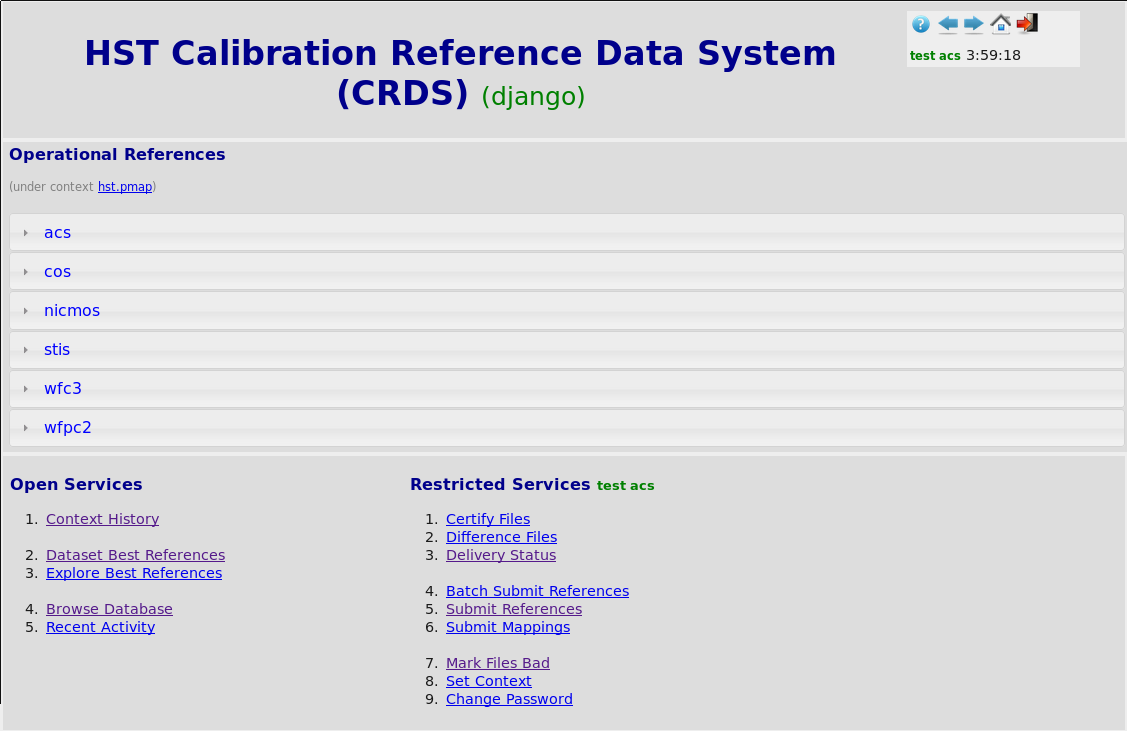
\includegraphics{web_index.png}}
\label{web_site_use:jwst-crds-stsci-edu}\end{figure}

Functions annotated with the word (alpha) are partially completed components of
a future build which may prove useful now.


\section{Operational References}
\label{web_site_use:operational-references}
The \emph{Operational References} table displays the references which are currently in use
by the pipeline associated with this web site.   The operational context is displayed
as a link `(under context \textless{}link\textgreater{})' immediately below Operational References.  Clicking
the link opens a details browser for that CRDS .pmap reference assignment rules file.
The operational context is the latest context in the Context History,  the one in
active use for pipeline processing by default.

Each instrument accordion opens into reference type accordions for that instrument.

Each type accordion opens into a table of reference files and the dataset parameters
they apply to.   Each reference file link opens into a details browser for that reference
file.


\section{Context History (more)}
\label{web_site_use:context-history-more}
The \emph{Context History} displays the last 4 CRDS contexts which were in operational use by
the pipeline associated with a CRDS server. Clicking on the \emph{(more)} link will bring up
the entire context history as a separate page as shown below:
\begin{figure}[htbp]
\centering

\scalebox{0.500000}{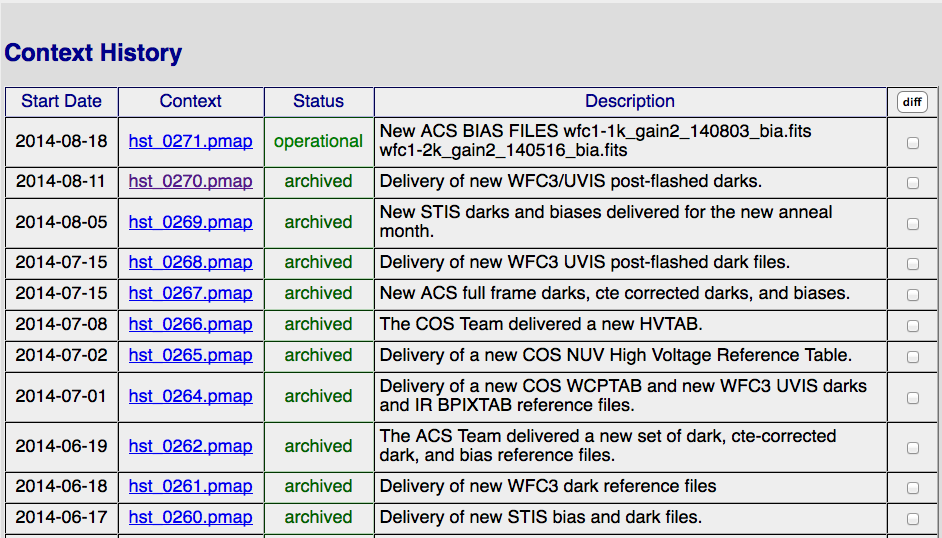
\includegraphics{web_context_history.png}}
\end{figure}

Clicking on a \emph{context} link (the .pmap name) opens a page containing the Historical References
for some point in the past,  similar to the Operational References display:
\begin{figure}[htbp]
\centering

\scalebox{0.500000}{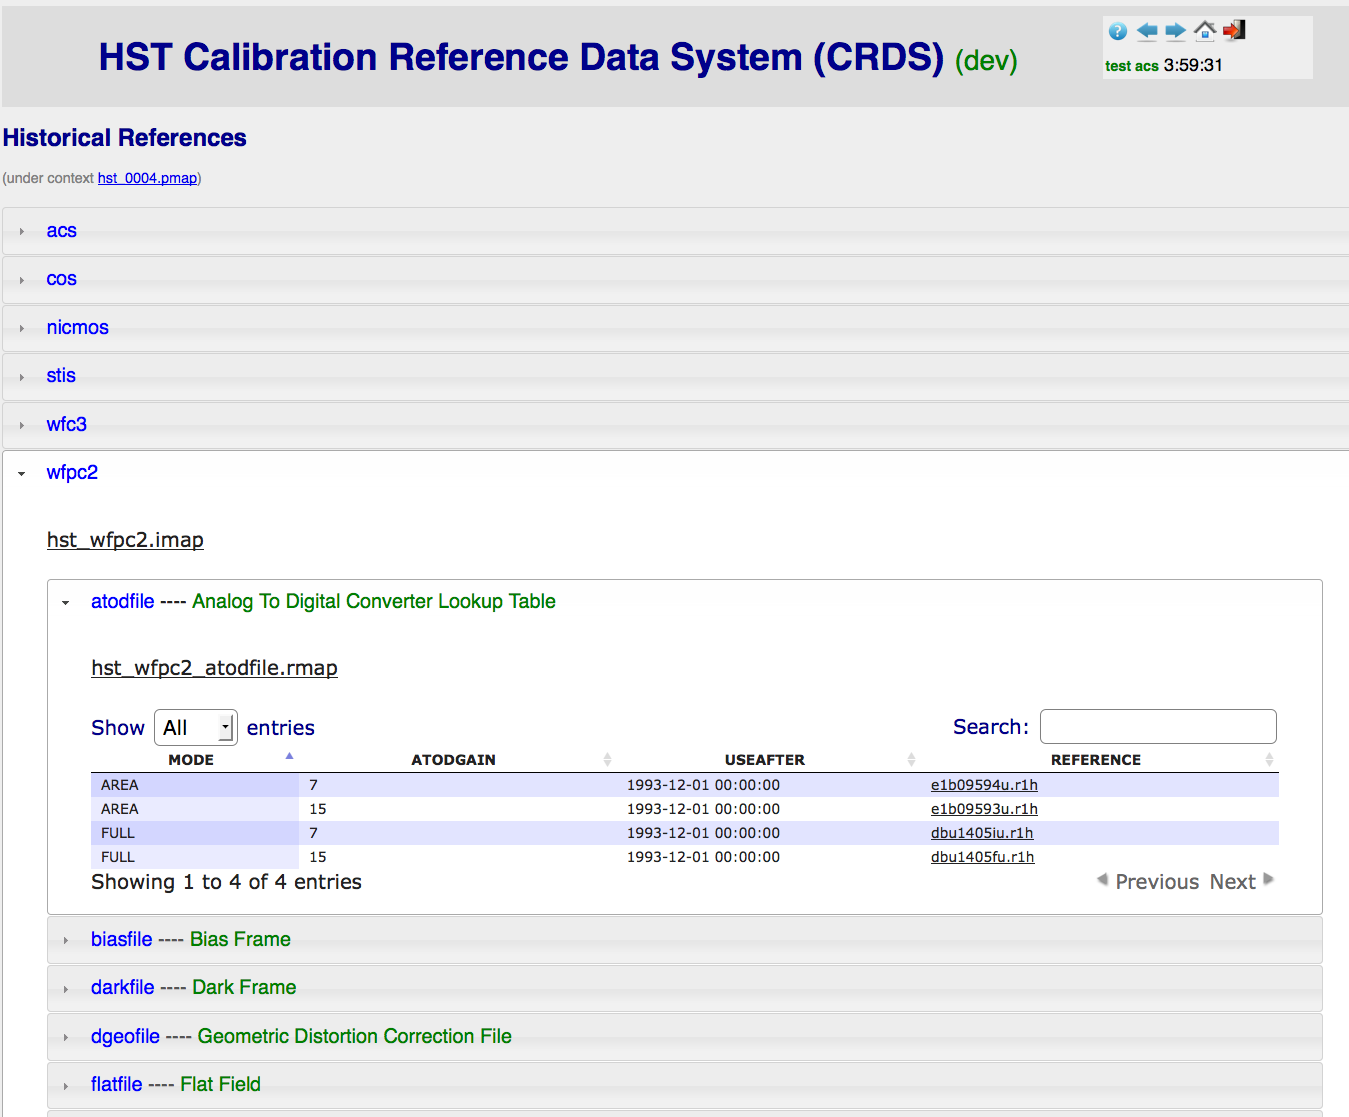
\includegraphics{web_context_table.png}}
\end{figure}

References are displayed in accordion panels for each instrument.   Opening the panel for
an instrument displays the reference types of that instrument.  Opening the panel for a type
displays particular reference files and matching parameters for that type.   Clicking on a particular
reference file brings up the CRDS browser page with the known details for that reference.


\subsection{Differencing contexts}
\label{web_site_use:differencing-contexts}
Click the \emph{diff} checkbox for any two contexts in the history and then click the diff button
at the top of the diff column.   This will display a difference page with an accorion panel
for each file which differed between the two contexts:
\begin{figure}[htbp]
\centering

\scalebox{0.500000}{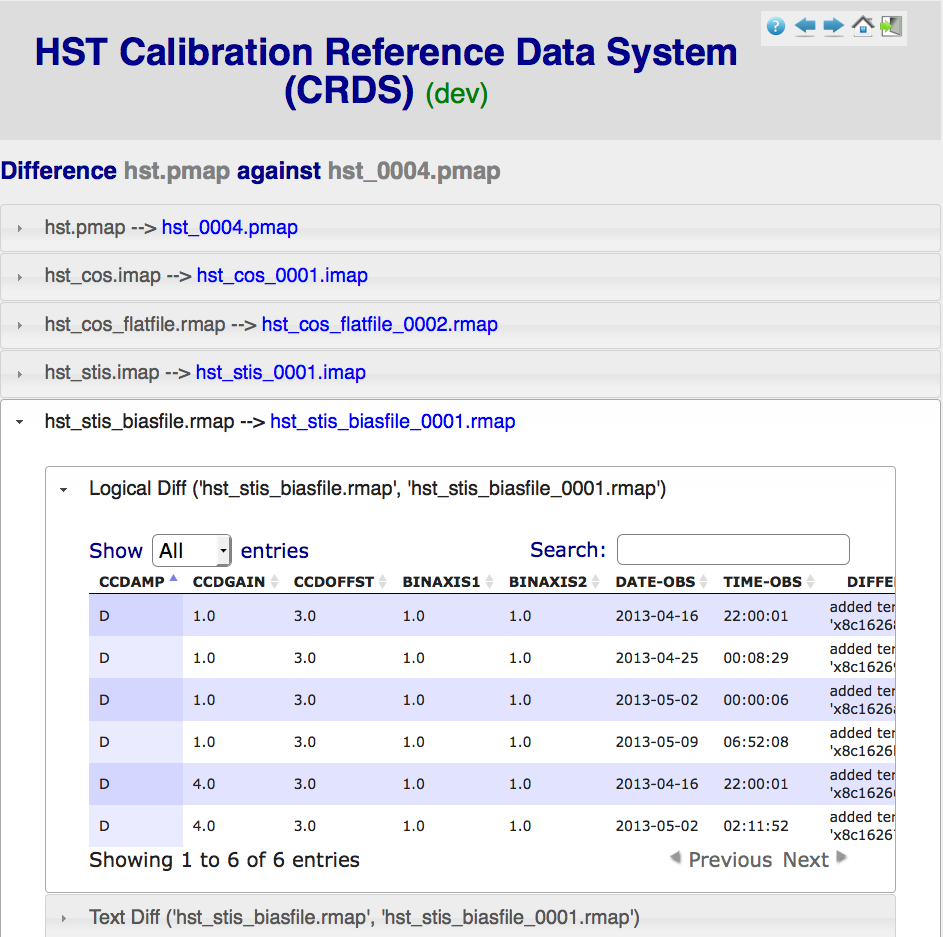
\includegraphics{web_context_difference.png}}
\end{figure}

Each file accordion opens into two accordions which display different views of the differences,
logical or textual.  The logical differences display a table of matching parameters and files
which were added, deleted, or replaced.   The textual differences show raw UNIX diffs of the
two rules files.


\section{Open Services}
\label{web_site_use:open-services}
The following functions are available for anyone with access to the CRDS web
server and basically serve to distribute information about CRDS files and
recommendations.   Initially,  the CRDS sites are only visible within the Institute.


\subsection{Dataset Best References}
\label{web_site_use:dataset-best-references}
The \emph{Dataset Best References} page supports determining the best references for
a single dataset with respect to one CRDS context.   Best references are based
upon a CRDS context and the parameters of the dataset as determined by the
dataset file itself or a database catalog entry.
\begin{figure}[htbp]
\centering

\scalebox{0.500000}{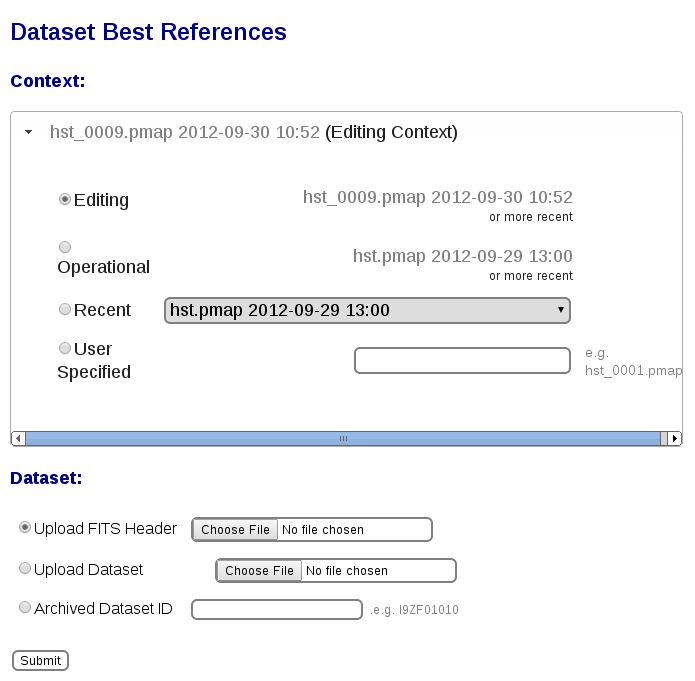
\includegraphics{web_dataset_bestrefs.png}}
\end{figure}


\subsubsection{Context}
\label{web_site_use:context}
The context defines the set of CRDS rules used to select best references.
\emph{Edit} is the default context from which most newly created contexts are derived.
\emph{Operational} is the context currently in use by the pipeline.   \emph{Recent} shows
the most recently created contexts.   \emph{User Specified} enables the submitter to
type in the name of any other known context.


\subsubsection{Dataset}
\label{web_site_use:dataset}

\paragraph{Upload FITS header}
\label{web_site_use:upload-fits-header}
Browser-side code can extract the FITS header of a dataset and upload it to the
server where best references are computed based on dataset parameters.   This
function is implemented in Javascript and reliant on HTML5;  it supports only
parameters present in the FITS primary header.   It avoids uploading most of the
dataset.   It is known to work in Firefox and Chrome but not IE or Safari-5.


\paragraph{Archived Dataset}
\label{web_site_use:archived-dataset}
Datasets can be specified by ID and their best reference input parameters will
be retrieved from the catalog.


\subsubsection{Dataset Best References Results}
\label{web_site_use:dataset-best-references-results}\begin{figure}[htbp]
\centering

\scalebox{0.500000}{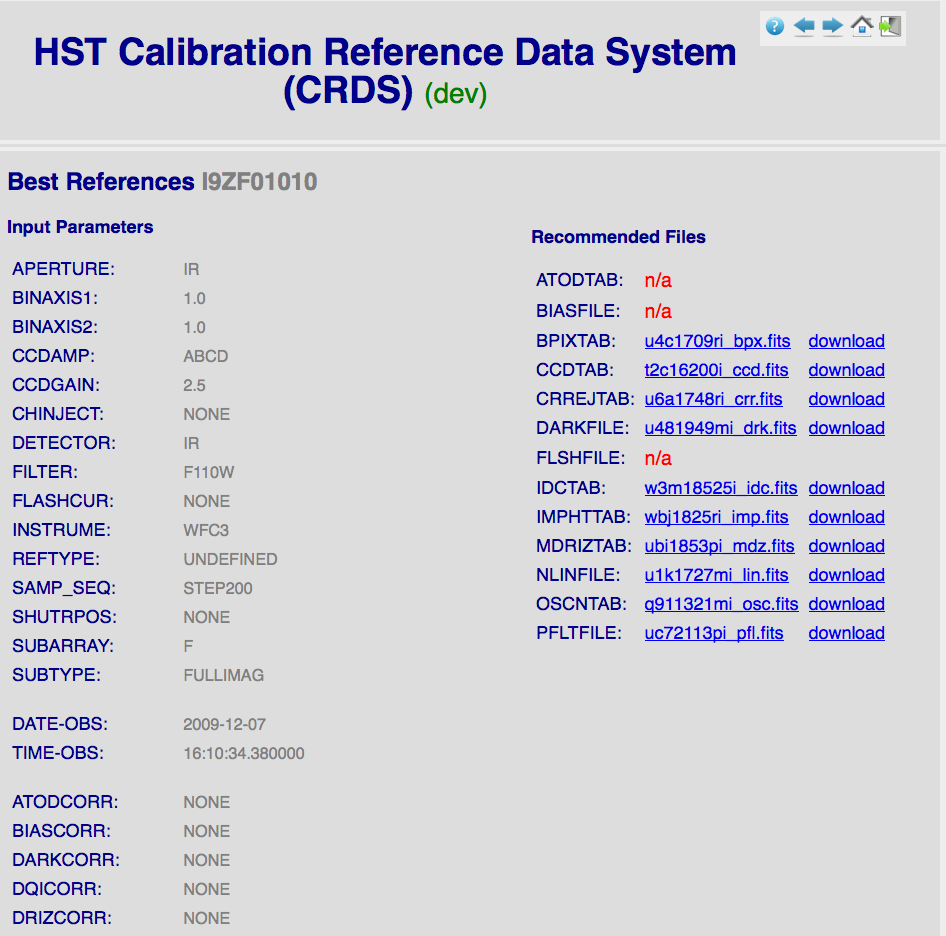
\includegraphics{web_dataset_bestrefs_results.png}}
\end{figure}

The results page for dataset best references displays the input parameters which
were extracted from the dataset header on the right side of the page.

Best reference recommendations are displayed on the left side of the page.


\subsection{Explore Best References}
\label{web_site_use:explore-best-references}
Explore Best References supports entering best references parameters directly
rather than extracting them from a dataset or catalog.   Explore best references
is essentially a sand box which lets someone evaluate what CRDS will do given
particular parameter values.  The explorer currently lists all parameters
which might be relevant to any mode of an instrument and has no knowledge of
default values.

The first phase of exploration is to choose a pipeline context and instrument
which will be used to define parameter choices:
\begin{figure}[htbp]
\centering

\scalebox{0.500000}{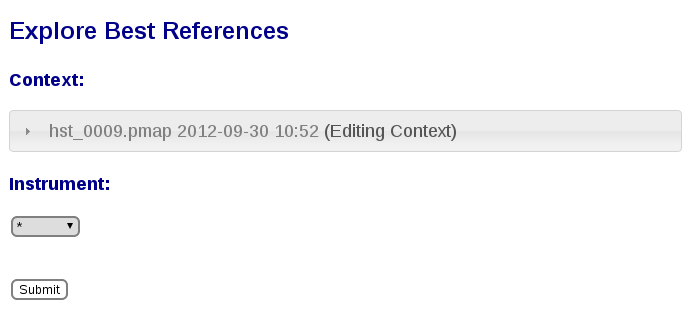
\includegraphics{web_explore_bestrefs.png}}
\end{figure}

The second phase is to enter the parameters of a dataset which are relevant
to best references selection.
\begin{figure}[htbp]
\centering

\scalebox{0.500000}{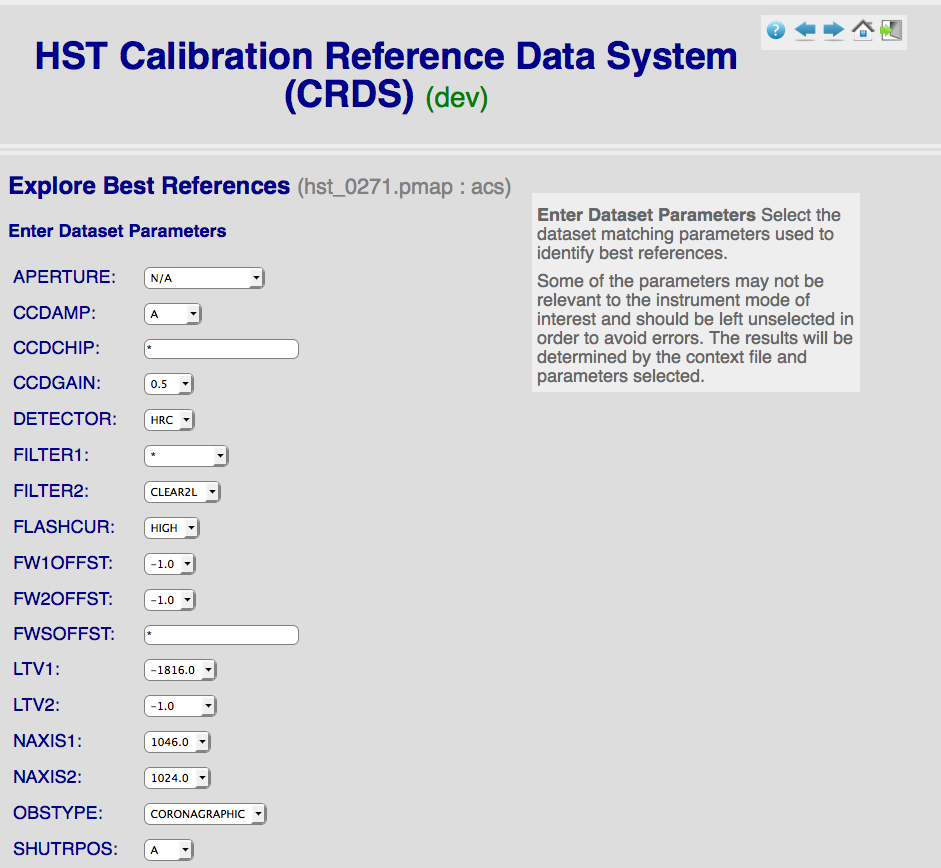
\includegraphics{web_explore_bestrefs_parameters.png}}
\end{figure}

The entered parameters are evaluated with respect to the given pipeline context
and best references are determined.   The results are similar or identical to
the \emph{Dataset Best References} results.


\subsection{Browse Database}
\label{web_site_use:browse-database}
The \emph{Browse Database} feature enables examining the metadata and computable
properties of CRDS reference and mapping files.
\begin{figure}[htbp]
\centering

\scalebox{0.500000}{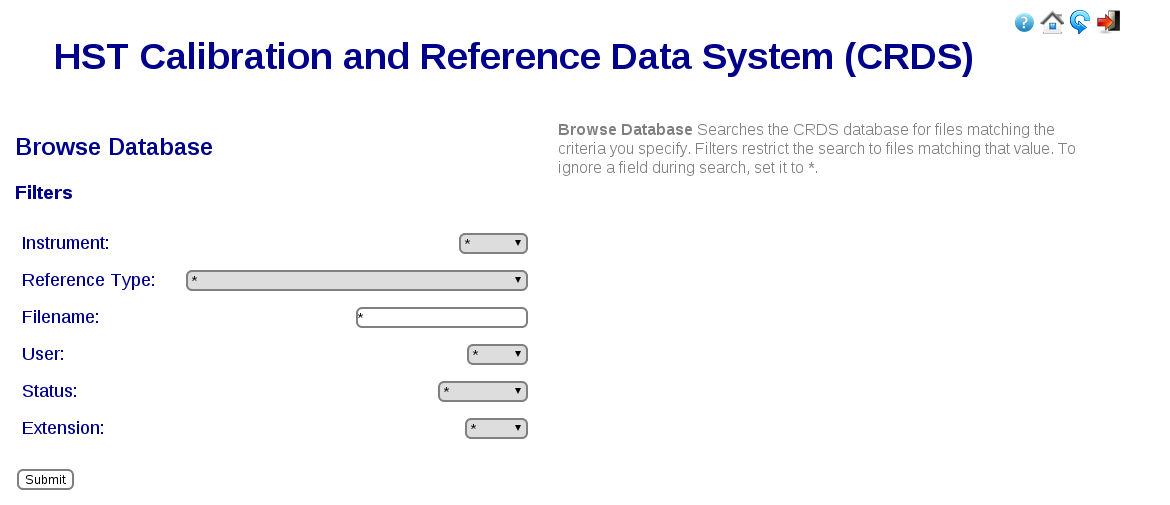
\includegraphics{web_browse_database.png}}
\end{figure}

The first phase is to enter a number of filters to narrow the number or variety
of files which are displayed.   Leaving any filter at the default value of *
renders that constraint irrelevant and all possible files are displayed with
respect to that constraint.   The result of the first phase is a table of files
which matched the filters showing their basic properties.
\begin{figure}[htbp]
\centering

\scalebox{0.500000}{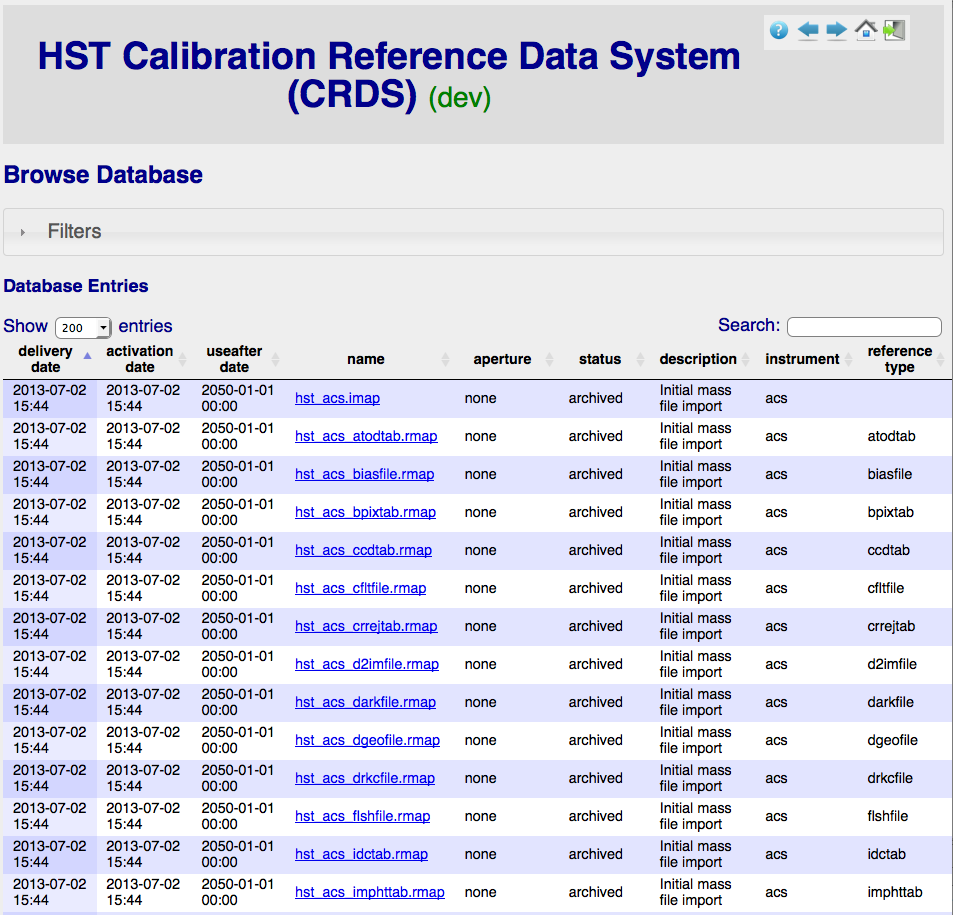
\includegraphics{web_browse_database_files.png}}
\end{figure}

The second phase is initiated by clicking on the filename link of any file
displayed in the table from the first phase.   Clicking on a filename link switches
to a detailed view of that file only:
\begin{figure}[htbp]
\centering

\scalebox{0.500000}{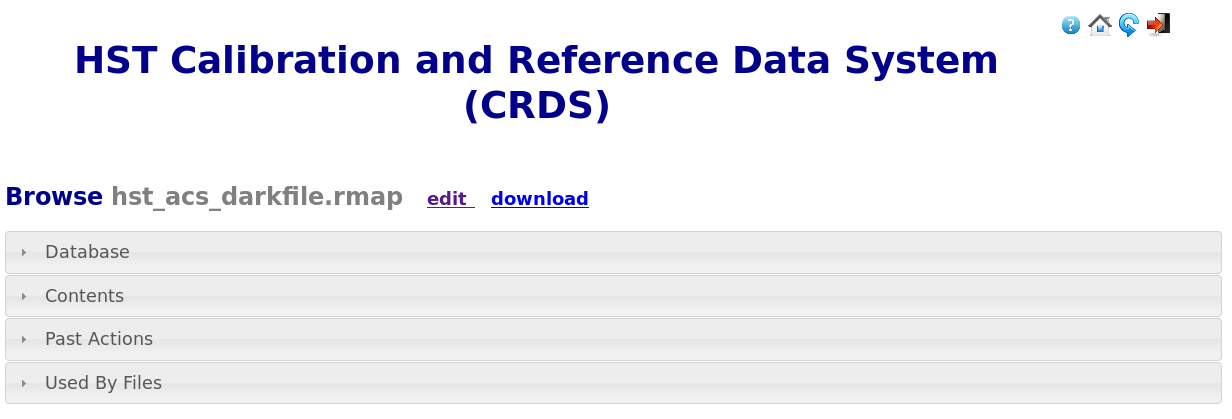
\includegraphics{web_browse_database_details.png}}
\end{figure}

The file details page has a number of accordion panes which open when you
click on them.  All file types have these generic panes:
\begin{itemize}
\item {} 
Database - lists a table of CRDS metadata for the file.

\item {} 
Contents - shows the text of a mapping or internal details about a reference file.

\item {} 
Past Actions  - lists website actions which affected this file.

\item {} 
Used By Files - list known CRDS files which reference this file.

\end{itemize}

Reference files have these additional panes:
\begin{itemize}
\item {} 
Certify Results - shows the results of crds.certify run on this reference now.

\item {} 
Lookup Patterns - lists the parameters sets which lead to this reference.

\end{itemize}


\subsection{Recent Activity}
\label{web_site_use:recent-activity}
The \emph{Recent Activity} view shows a table of the actions on CRDS files which
are tracked.  Only actions which change the states of files in some way are
tracked:
\begin{figure}[htbp]
\centering

\scalebox{0.500000}{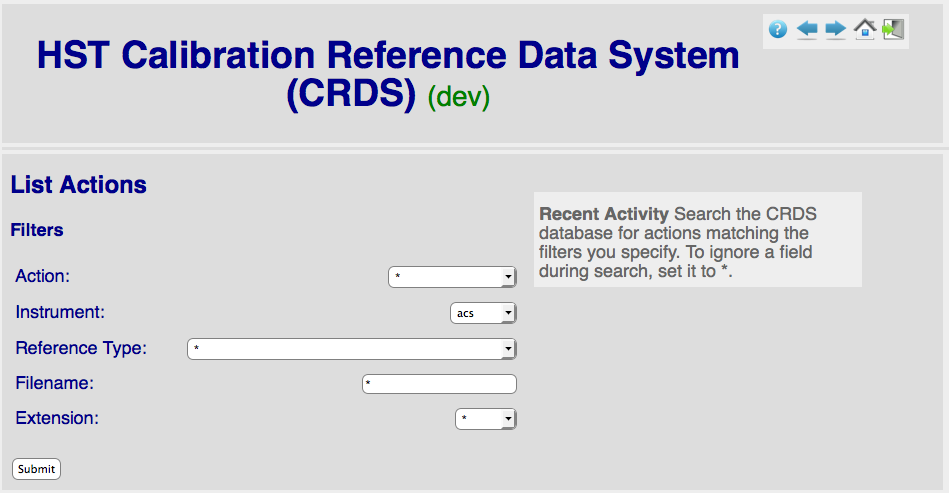
\includegraphics{web_recent_activity.png}}
\end{figure}

The first page lists a number of constraints which can be used to choose
activities of interest.   To ignore any constraint,  leave it set at the default
value of *.   The result of the activity search is a table of matching actions:
\begin{figure}[htbp]
\centering

\scalebox{0.500000}{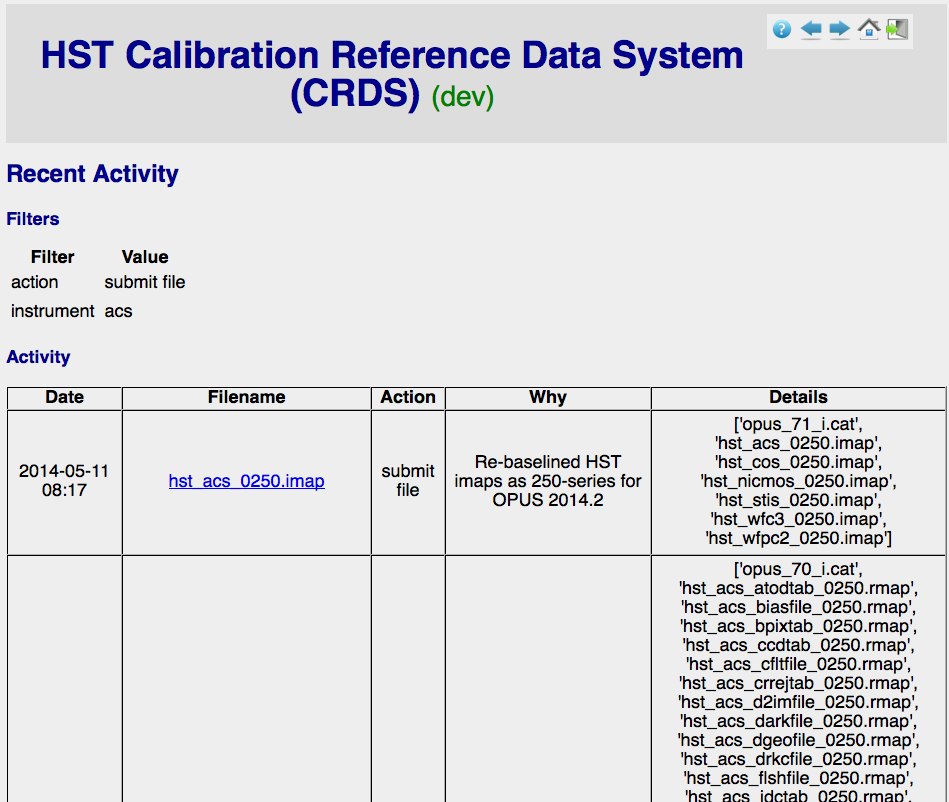
\includegraphics{web_recent_activity_results.png}}
\end{figure}

The details vary by the type of action,  in this case showing the original name
of a file prior to submission to CRDS and the assignment of its official name.


\section{Private Functions}
\label{web_site_use:private-functions}
The following functions are restricted to users with accounts on the CRDS website
and support the submission of new reference and mapping files and maintenance
of the overall site.   Private functions are only visible to users who have
successfully logged in.


\subsection{Login and Instrument Locking}
\label{web_site_use:login-and-instrument-locking}
Typical batch file submissions automatically generate instrument and pipeline context
files,  as well as .rmaps.   To preclude the possibility of multiple users submitting
files from the same instrument at the same time,  and possibly creating conflicting
rules,  users lock instruments when they log in.
\begin{figure}[htbp]
\centering

\scalebox{0.500000}{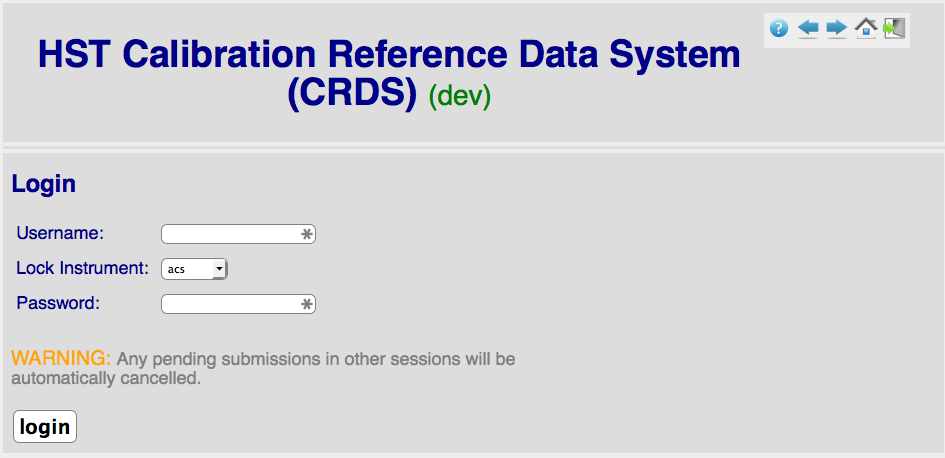
\includegraphics{web_login.png}}
\end{figure}

When a user logs in,  the instrument they've locked and the time remaining on the
lock are displayed below the login (now logout) button:
\begin{figure}[htbp]
\centering

\scalebox{0.500000}{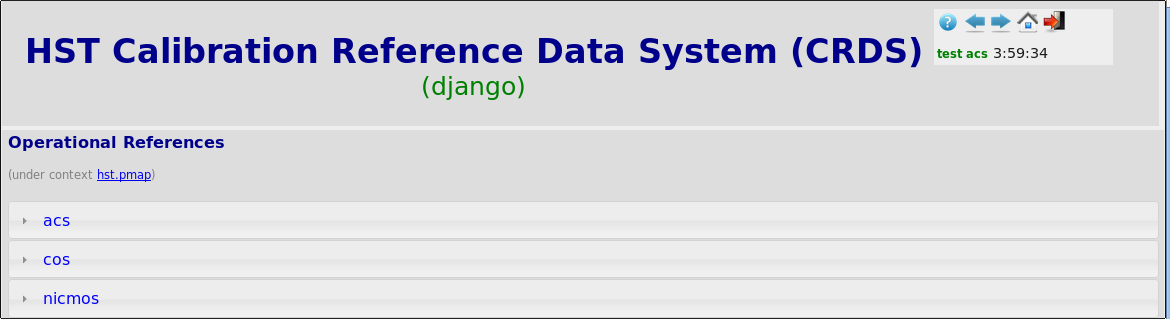
\includegraphics{web_logged_in.png}}
\end{figure}

The time displayed is the relative time remaining on the lock reservation,  nominally
around 4 hours with the current server configuration.

When the user performs an action on the website,  their lock timer is reset to its maximum value.
As time passes without action,  the lock timer counts down.  When the lock timer reaches zero,
the lock is automatically released and any on-going file submission is cancelled.   Files which
have been uploaded for a cancelled submission are left in the upload area.

Other users who attempt to login while an instrument is locked will be denied.

When a file submission is being performed,  it must be \emph{confirmed} within the timeout period
or the file submission will be cancelled.

Care should be taken with the locking mechanism and file submissions.  \textbf{DO NOT}:
\begin{itemize}
\item {} 
Don't login from multiple browsers or sites.   The last browser/site you log in from will steal the
lock from the original login, cancel any original file submission,  and force a logout in the original browser.

\item {} 
Don't leave the page during an ongoing file submission,  wait for it to finish.   Opening other browser
tabs should be fine.

\item {} 
Don't attempt to login for more than one instrument at a time.  One user is assigned one and only one lock.

\item {} 
Don't attempt to perform multiple file submissions for the same instrument at the same time.  Finish
and confirm or cancel each file submission before proceeding with the next.

\end{itemize}


\subsection{Certify Files}
\label{web_site_use:certify-files}
\emph{Certify File} runs crds.certify on the files in the ingest directory.
\begin{figure}[htbp]
\centering

\scalebox{0.500000}{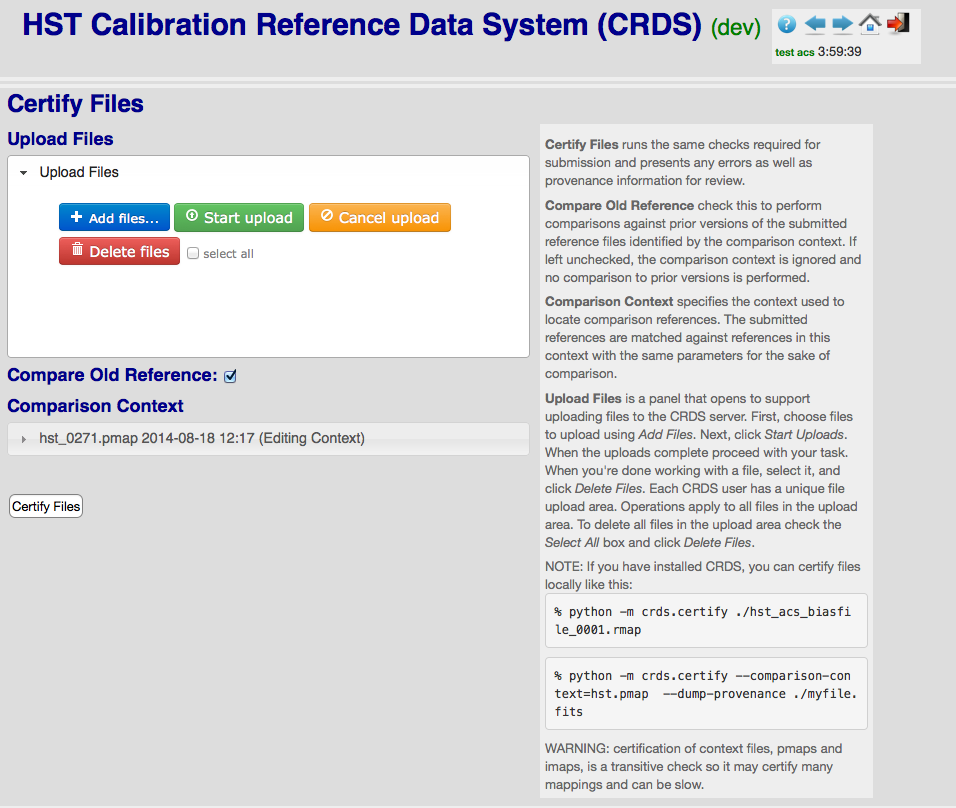
\includegraphics{web_certify_file.png}}
\end{figure}

If the certified file is a reference table,  the specified context is used to
locate a comparison file.


\subsection{Mark Files Bad}
\label{web_site_use:mark-files-bad}
\emph{Mark Files Bad} supports marking a file as scientifically invalid and
also supports reversing the decision and marking it good once more.

The CRDS procedure for marking files bad requires three steps:
\begin{enumerate}
\item {} 
Create a clean context which does not contain any prospective bad files.

\item {} 
Make the clean context operational using Set Context.

\item {} 
Mark the prospective bad files actually bad using Mark Bad Files.

\end{enumerate}

Following this procedure maintains the invariant that the operational context
contains no known bad files.   The designation as bad files does not take
effect until any local CRDS cache is synchronized with the server.

Creating a clean context can be done in arbitrary ways,  but the two most
common ways will likely be:
\begin{enumerate}
\item {} 
Submit replacement files for the bad files to create a clean context.

\item {} 
Use Delete References to generate a new context without the bad files.

\end{enumerate}
\begin{figure}[htbp]
\centering

\scalebox{0.500000}{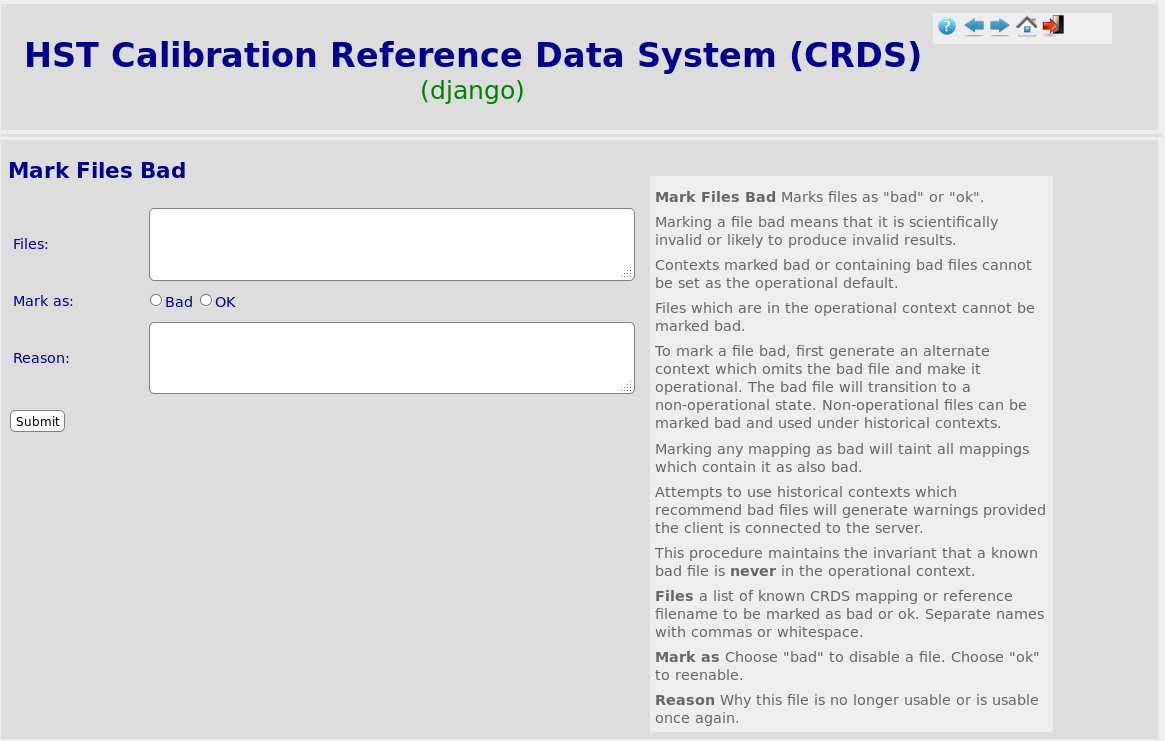
\includegraphics{web_mark_files_bad.png}}
\end{figure}

Marking a rules file (mapping) as bad implicitly marks all the files
which refer to it as bad.  Hence,  marking a .rmap as bad will make
any .imap which refers to it bad as well,  and will also taint all .pmaps
which refer to the bad .imaps.   Whenever a rules file is marked bad,
a warning is issued when the containing context is used.

Marking a reference file as bad is a more precise technique which invalidates
only that reference in every context that includes it.  Warnings are issued
related to the bad reference only when the reference is actually recommended by
CRDS.

By default, recommendation of bad files is an error.  The default
behaviour can be overrideden, allowing use of bad rules or references with a
warning, by setting environment variables: \emph{CRDS\_ALLOW\_BAD\_RULES} and/or
\emph{CRDS\_ALLOW\_BAD\_REFERENCES} or by using command line switches for
crds.bestrefs: \emph{--allow-bad-rules} and \emph{--allow-bad-references}.


\subsection{Delete References}
\label{web_site_use:delete-references}
\emph{Delete References} supports supports removing references (but not rules) from
a context generating a new context.  Delete References provides one
straightforward way to generate clean rules prior to marking the deleted files
as bad.
\begin{figure}[htbp]
\centering

\scalebox{0.500000}{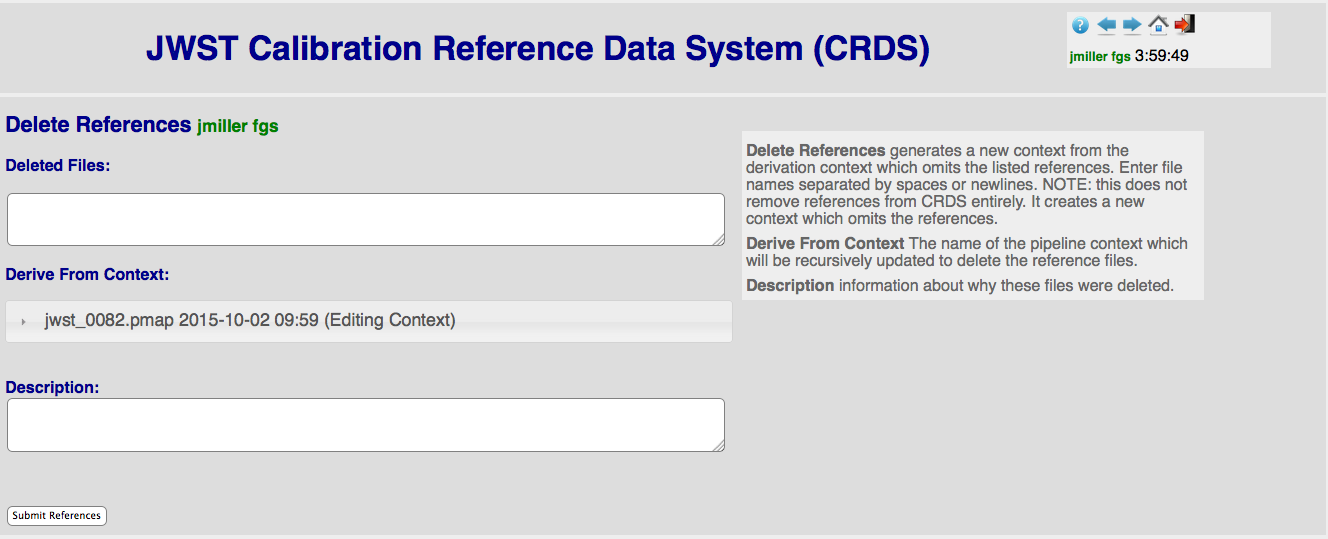
\includegraphics{web_delete_references.png}}
\end{figure}

Delete References does not remove the files from CRDS, it only removes them
from the specified set of rules.  The references remain available under any
contexts which still refer to them.

Once references have been replaced or deleted from the operational context and
the new context is made operational using Set Context, the deleted or replaced
references can be marked as scientifically invalid using Mark Files Bad.

Files are specified for Delete References by listing their names in the Deleted
Files field of the input form, separated by spaces, commas, and/or newlines.

Changes to rules which result from delete references are presented on a results
page which must be confirmed or cancelled as with other file submissions.


\subsection{Add References}
\label{web_site_use:add-references}
\emph{Add References} supports adding existing CRDS references to a CRDS context
which does not contain them already.  Add References is the inverse of Delete
References and generates new CRDS rules without requiring the resubmission of
files to CRDS.
\begin{figure}[htbp]
\centering

\scalebox{0.500000}{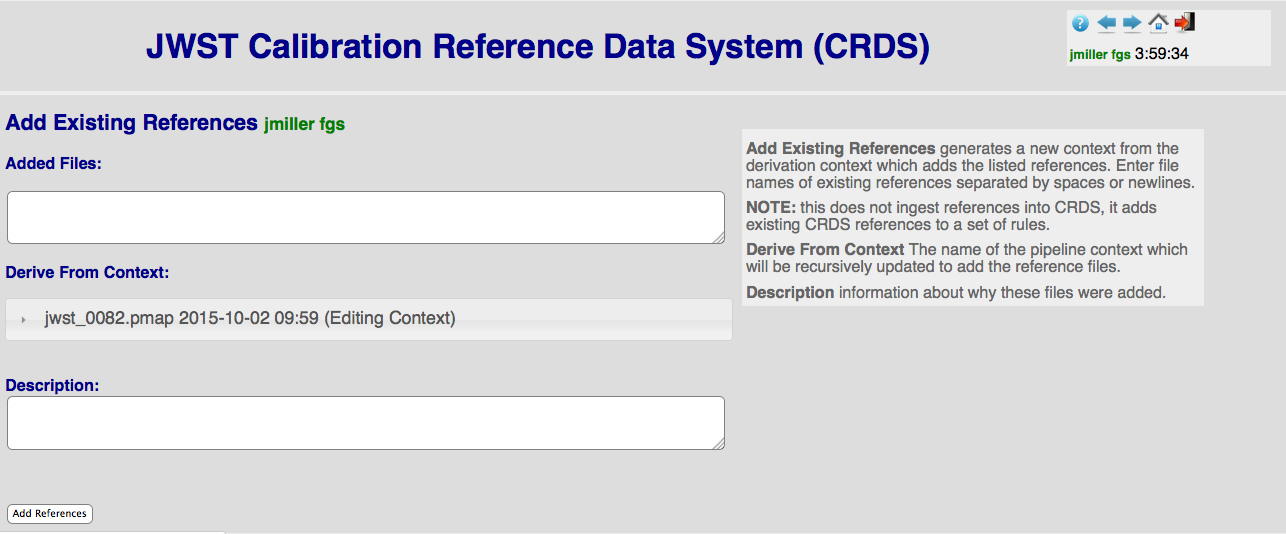
\includegraphics{web_add_references.png}}
\end{figure}

Add references can be used to undo the effects of Delete References in a
perhaps distant descendant context containing other changes.  Add references
can also be used to add tested references from a branched context into the
current operational context.

Files are specified for Add References by listing their names in the Added
Files field of the input form, separated by spaces, commas, and/or newlines.

Changes to rules which result from add references are presented on a results
page which must be confirmed or cancelled as with other file submissions.
Rules changes from add references should be carefully reviewed to ensure that
the resulting rmap update is as intended.  In particular, other rmap
differences from a branched context are not added, so additional test
parameters or other header and structural changes of any test rmap are not
carried over by Add References,  only the reference files themselves.


\subsection{Set Context}
\label{web_site_use:set-context}
\emph{Set Context} enables setting the operational and edit contexts.
\begin{figure}[htbp]
\centering

\scalebox{0.500000}{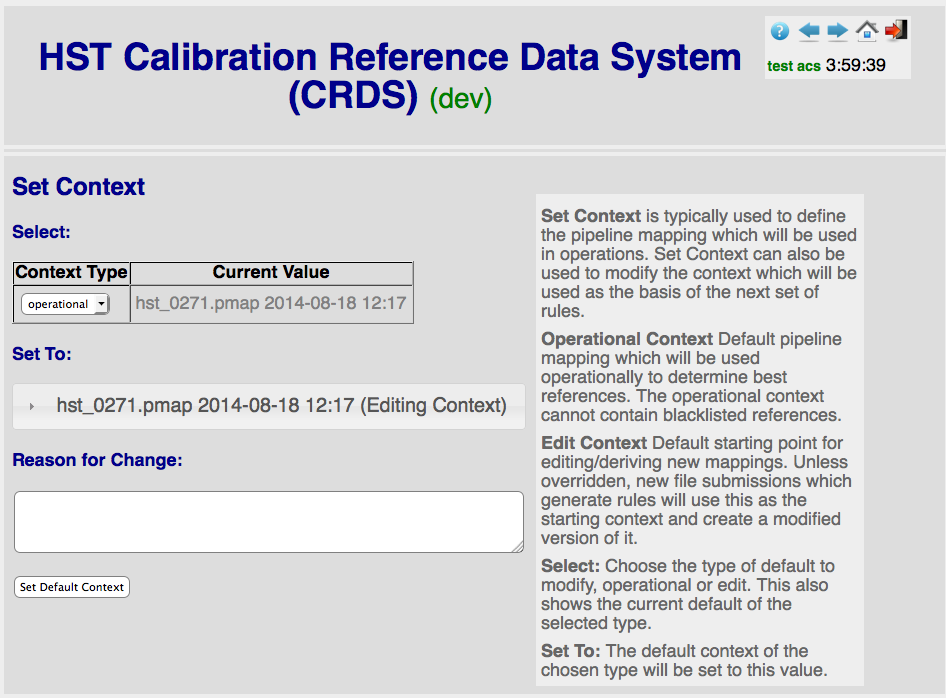
\includegraphics{web_set_context.png}}
\end{figure}

CRDS enables contexts to be pre-positioned before their adoption as the default
for processing by the pipeline.  Only by using Set Context will an available
context become the default for processing.

Setting the operational context makes the specified context the default for
processing coordinated by this server.  Setting the operational context creates
a new entry at the top of the Context History.

Setting the edit context makes the specified context the default starting point
for future contexts created during file submission.


\subsection{Batch Submit References}
\label{web_site_use:batch-submit-references}
\emph{Batch Submit References} is intended to handle the majority of CRDS reference
submissions with a high degree of automation.   This page accepts a number of
reference files and metadata which is applied to all of them.   The specified
reference files are checked on the server using crds.certify and if they pass
are submitted to CRDS.   All of the submitted references must be of the same
reference type,  i.e. controlled by the same .rmap file.   Tabular reference
files are checked with respect to the derivation context by crds.certify.
\begin{figure}[htbp]
\centering

\scalebox{0.500000}{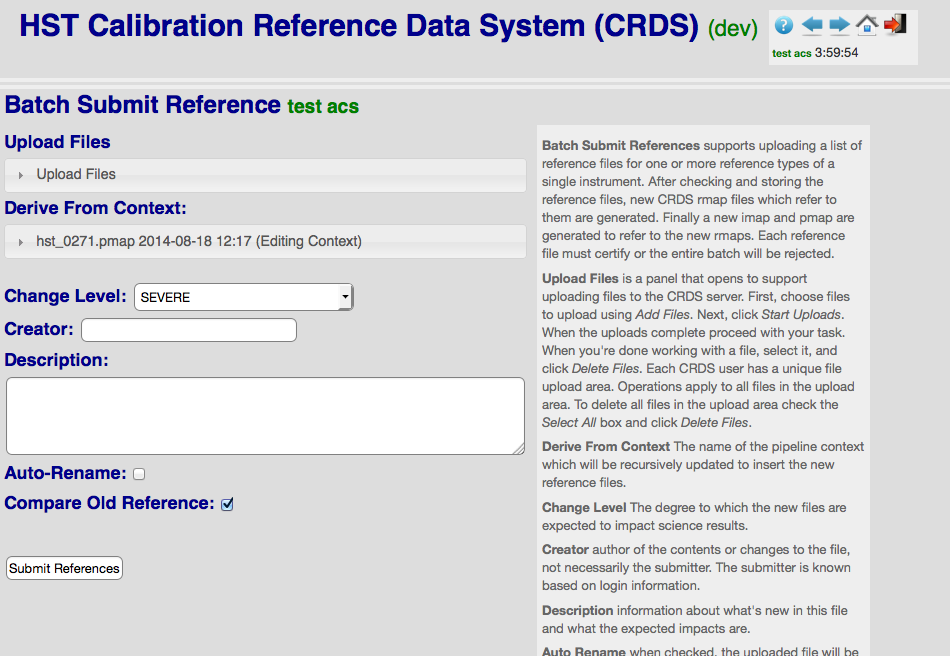
\includegraphics{web_batch_submit_references.png}}
\end{figure}


\subsubsection{Upload Files}
\label{web_site_use:upload-files}
The first task involved with \emph{Batch Submit References} is transferring the
submitted files to the server.  For CRDS build-2,  there are two approaches for
getting files on the server,  web based and shell based.   Both approaches
involve transferring files to an ingest directory in the CRDS filestore.  Each
CRDS user will have their own ingest directory.   Initially the only user is
``test''.   This section applies equally to all of the file submission pages that
have an \emph{Upload Files} accordion.


\paragraph{Web Approach}
\label{web_site_use:web-approach}
On the file submission pages,  the \emph{Upload Files} accordion opens to support
uploading submitted files to a user's CRDS ingest directory via the browser.
\begin{figure}[htbp]
\centering

\scalebox{0.500000}{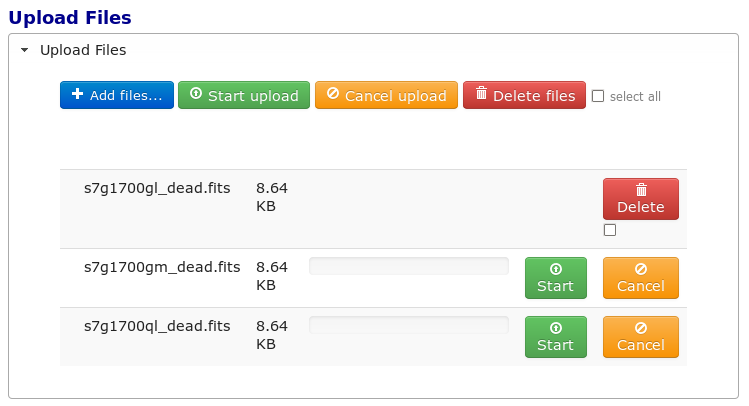
\includegraphics{web_upload_files.png}}
\end{figure}

Uploading files is accomplished by:
\begin{itemize}
\item {} 
Opening the accordion panel by clicking on it.

\item {} 
Add files to the upload list by clicking on the \emph{Add Files...} button.  Alternately for modern browsers (Chrome) drag-and-drop files from your desktop to the upload accordion.

\item {} 
Click \emph{Start Upload} to initiate the file transfer.   You should see a progress bar(s) showing the status of the upload(s).   When the upload successfully completes the buttons will change to \emph{delete}.

\item {} 
Click \emph{Delete} for any file added by mistake or for failed uploads.

\item {} 
Click \emph{Cancel Upload} to abort a file transfer during the upload.

\item {} 
Close the accordion panel by clicking on it.

\end{itemize}

\textbf{IMPORTANT}  Just adding files to the file list does not upload them.   You
must click \emph{Start upload} to initiate the file transfer.   In the screenshot above,
the file with the \emph{delete} button next to it is already on the server in the
ingest directory.   The files with \emph{start} and \emph{cancel} buttons next to them have
only been declared as candidates for upload.   To finish uploading all 3 files,
check \emph{select all} and click \emph{Start upload}.


\paragraph{Shell Approach}
\label{web_site_use:shell-approach}
In the shell approach a user must login to UNIX (in some fashion) and transfer
files into their CRDS ingest directory manually.   The nominal approach
for doing this is to use the cp or scp commands.   For instance,  from my home,
having already set up ssh and scp access, I might say:

\begin{Verbatim}[commandchars=\\\{\}]
\PYGZpc{} scp /this\PYGZus{}delivery/*.fits   dmsinsvm.stsci.edu:/ifs/crds/hst/test/server\PYGZus{}files/ingest/mcmaster
\end{Verbatim}

to copy references into my ingest directory \emph{as-if} I had uploaded them through
the uploads panel.

Abstractly this is:

\begin{Verbatim}[commandchars=\\\{\}]
\PYGZpc{} scp \PYGZlt{}submitted reference files...\PYGZgt{}   \PYGZlt{}host\PYGZgt{}:/ifs/crds/hst/\PYGZlt{}pipeline\PYGZgt{}/server\PYGZus{}files/ingest\PYGZlt{}crds\PYGZus{}username\PYGZgt{}
\end{Verbatim}

where pipeline is `test' or `ops'.

The submitted reference files should now be in the ingest directory for \emph{HST} test server
user \emph{mcmaster}.   Once the files are in the ingest directory,  the CRDS web server
will behave as if they had been uploaded through web interface.  Refreshing the
file submission web page should make manually copied files show up in the
\emph{Upload Files} accordion.

The purpose of using cp or scp is to improve the efficiency and reliability of
the file transfers should those become an issue.  Telecommuters working offsite by VPN
would face a situation where submitted files are downloaded to their home computer via
VPN and then uploaded to the CRDS server via their browser.

Files transferred to the ingest directory via shell should
still be removeable using the \emph{Upload Files} delete buttons.


\subsubsection{Derive From Context}
\label{web_site_use:derive-from-context}
The specified context is used as the starting point for new automatically
generated context files and also determines any predecessors of the submitted
references for comparison during certification.   If all the submitted reference
files pass certification,  a new .rmap, .imap, and .pmap are generated
automatically to refer to the newly entered references.    Based on their
header parameters,  references are automatically assigned to appropriate
match locations in the .rmap file.
\begin{figure}[htbp]
\centering

\scalebox{0.500000}{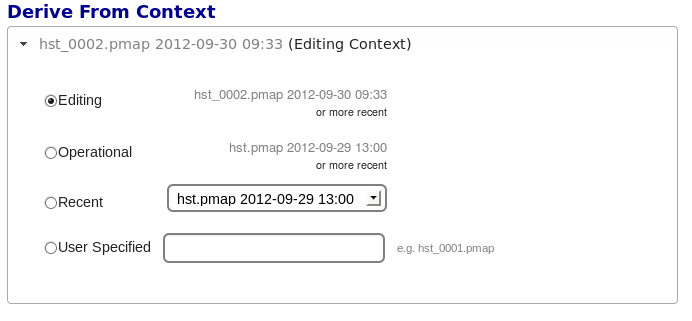
\includegraphics{web_derive_from_context.png}}
\end{figure}

There are two special contexts in CRDS which are tracked:


\paragraph{Edit Context}
\label{web_site_use:edit-context}
Edit Context is the default context used for editing.   Whenever a new .pmap is created or
added,  it becomes the editing context from which other .pmaps are derived by
default.


\paragraph{Operational Context}
\label{web_site_use:operational-context}
Operational Context is the .pmap which is nominally in use by
the pipeline.  Generally speaking,  multiple contexts might be added to CRDS as
the Edit Context long before they become operational.


\paragraph{Recent}
\label{web_site_use:recent}
Recent lists a number of recently added contexts based on delivery time.


\paragraph{User Specified}
\label{web_site_use:user-specified}
Any valid CRDS context can be typed in directly as User Specified.


\subsubsection{Auto Rename}
\label{web_site_use:auto-rename}
Normally files uploaded to CRDS will be assigned new unique names.   During side-by-side
testing with CDBS,  \emph{Auto Rename} can be deselected so that new files added to CRDS
retain their CDBS names for easier comparison.  The CRDS database remembers both
the name of the file the submitter uploaded as well as the new unique name.


\subsubsection{Compare Old Reference}
\label{web_site_use:compare-old-reference}
When checked CRDS will certify incoming tabular references against the files
they replace with respect to the derivation context.   For other references this
input is irrelevant and ignored.


\subsubsection{Results}
\label{web_site_use:results}\begin{figure}[htbp]
\centering

\scalebox{0.500000}{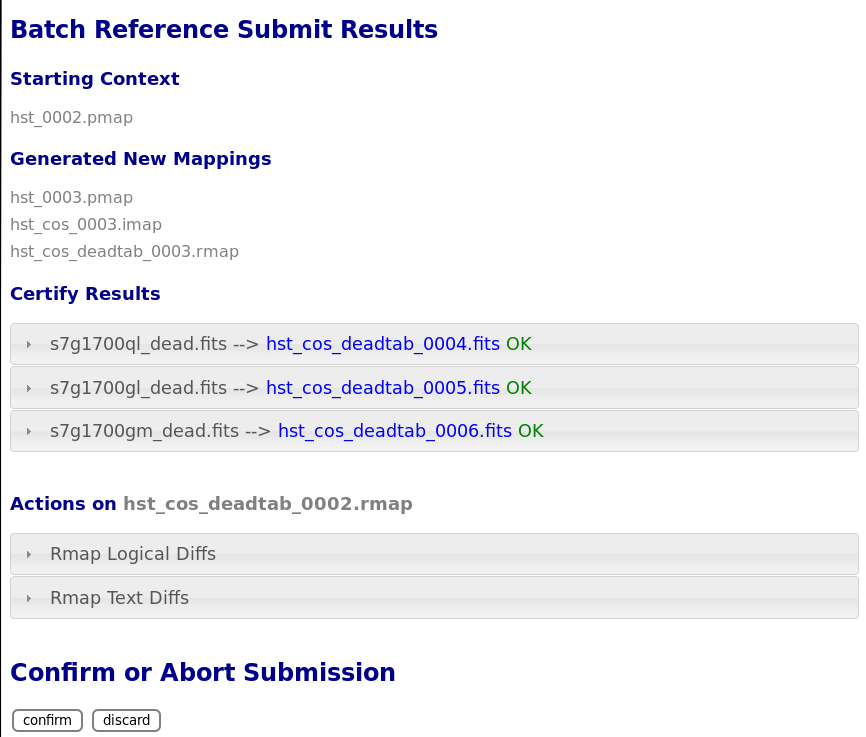
\includegraphics{web_batch_submit_results.png}}
\end{figure}

The results page lists the following items:
\begin{itemize}
\item {} 
\emph{Starting Context} is the context this submission derove from.

\item {} 
\emph{Generated New Mappings} lists the new mapping files which provide the generated context for using the submitted references.

\item {} 
\emph{Actions on Rmap} provides two accordions showing how the rmap controlling the submitted references was modified.   The logical differences accordion has a table of actions,  either \emph{insert} for completely new files or \emph{replace} for files which replaced an existing file.   The text differences are essentially output from UNIX \emph{diff} for the old and new rmaps.

\item {} 
\emph{Certify Results} has an accordion panel for each submitted reference file which contains the results from crds.certify.   The submitted name of each file is listed first,  followed by any official name of the file assigned by CRDS.   The status of the certification can be ``OK'' or ``Warnings''.   Warnings should be reviewed by opening the accorion panel.

\end{itemize}

\textbf{IMPORTANT}  The results page only indicates the files which will be added to
CRDS if the submission is \emph{confirmed}.   Prior to confirmation of the submission,
neither the submitted references nor the generated mappings are officially in CRDS.
Do not \emph{leave the confirmation page} prior to confirming.


\subsubsection{Collisions}
\label{web_site_use:collisions}
Under some circumstances,  a \emph{Collision Warning} accordion will be present.
It should be carefully examined to ensure that overlapping edits of the
same context file have not occurred.   Overlaps can be resolved by cancelling
the current submission and re-doing it, or by accepting the current submission
and manually correcting the mappings involved.   Failure to correctly resolve
a collision will most likely result in one of two sets of conflicting changes
being lost.
\begin{figure}[htbp]
\centering

\scalebox{0.500000}{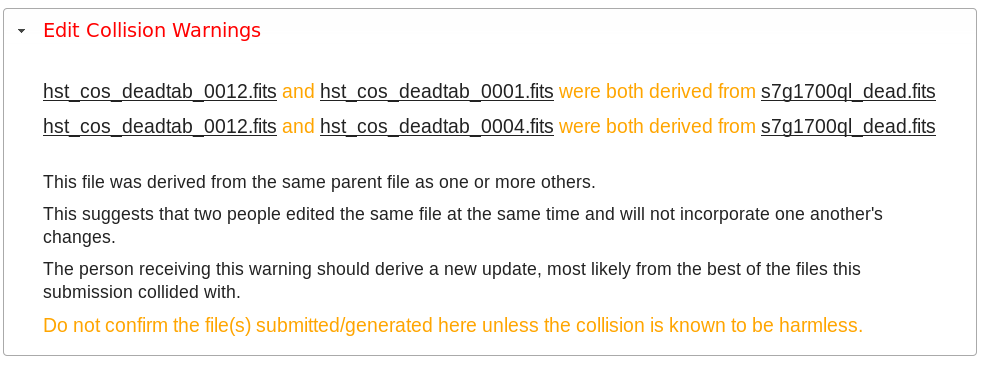
\includegraphics{web_collision_warnings.png}}
\end{figure}

Collision tracking for CRDS mappings files is done based upon header fields,
nominally the \emph{name} and \emph{derived\_from} fields.  These fields are automatically
updated when mappings are submitted or generated.

Collision tracking for reference files is currently filename based.   The submitted
name of a reference file is assumed to be the same as the file it
was derived from.   This fits a work-flow where a reference is first downloaded
from CRDS, modified under the same name,  and re-uploaded.   Nominally,  submitted
files are automatically re-named.


\subsubsection{Confirm or Discard}
\label{web_site_use:confirm-or-discard}
If everything looks good the last step is to click the \emph{Confirm} button.
Clicking the Confirm button finalizes the submission process,  submits the files
for archive pickup,  and makes them a permanent part of CRDS visible in the
database browser and potentially redistributable.   A confirmed submission
cannot be revoked,  but neither will it go into use until the pipeline or a
user explicitly requests it.

\emph{Discarding} a batch submission based on warnings or bad rmap modifications
removes the submission from CRDS.   In particular temporary database records
and file copies are removed.

Following any CRDS pipeline mapping submission,  the default \emph{edit} context
is updated to that pipeline mapping making it the default starting point for
future submissions.


\subsection{Submit References}
\label{web_site_use:submit-references}
\emph{Submit References} provides a lower level interface for submitting a list of
references.   No mappings are generated to refer to the submitted files.
Submitted references must still pass through crds.certify.
\begin{figure}[htbp]
\centering

\scalebox{0.500000}{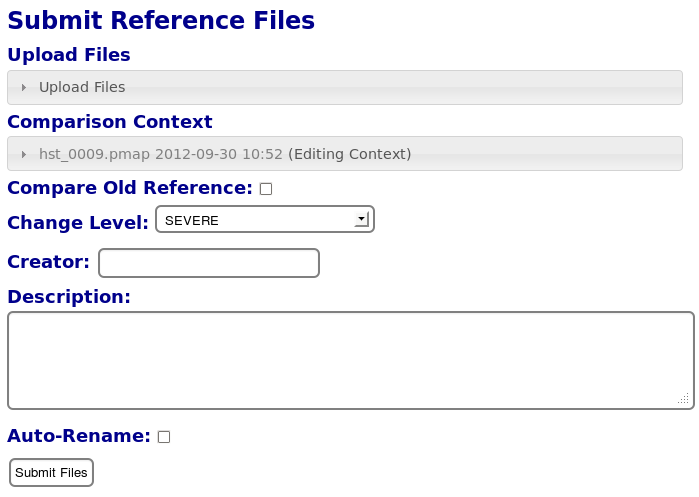
\includegraphics{web_submit_references.png}}
\end{figure}


\subsection{Submit Mappings}
\label{web_site_use:submit-mappings}
\emph{Submit Mappings} provides a basic interface for submitting a list of mapping
files which don't have to be related.   This can be used to submit context files
which refer to files from \emph{Submit References} and with fewer restrictions on
allowable changes.   Typically only .rmaps are submitted this way.   Mappings
submitted this way must also pass through crds.certify.
\begin{figure}[htbp]
\centering

\scalebox{0.500000}{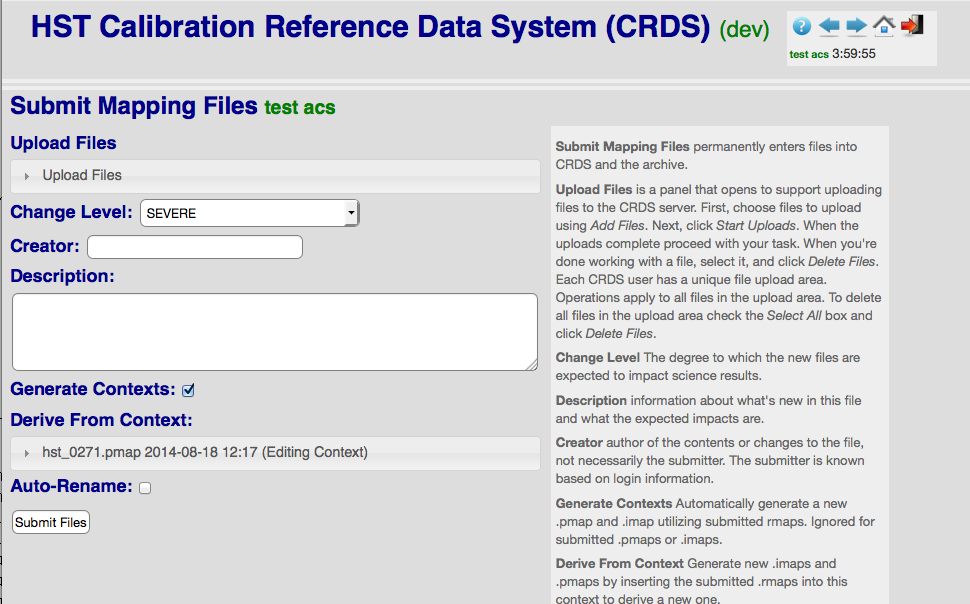
\includegraphics{web_submit_mappings.png}}
\end{figure}


\subsubsection{Mapping Change Procedure}
\label{web_site_use:mapping-change-procedure}
The nominal process used to modify CRDS mappings is to:

1. Download the mapping to be used as a baseline for the revised version.
Leave the name as-is.  The download can be accomplished by using the crds.sync
tool to download the file to a local cache, or by browsing to the file's
details page and using the \emph{download} link near the top of the page.  Likewise
the source file can be copied directly from the shared on site default
readonly cache.   This download, don't rename, upload process is used to
automatically maintain the derivation history of mappings in their headers,
the name field is progagated down to the derived\_from field to track the
source mapping prior to renaming the new mapping.

2. Modify the mapping in a text editor implementing required changes.  Use
care editing mappings since many aspects of the mapping cannot be verified by
crds.certify.   Where possible match values are validated against CRDS .tpn
files or JWST data model schema.

3. Run crds.certify on the resulting mapping, using the current operational
context as the point of comparison:

\begin{Verbatim}[commandchars=\\\{\}]
\PYGZpc{} python \PYGZhy{}m crds.certify ./jwst\PYGZus{}miri\PYGZus{}dark\PYGZus{}0004.rmap  \PYGZhy{}\PYGZhy{}comparison\PYGZhy{}context jwst\PYGZhy{}operational
\end{Verbatim}

4. During iteration, run crds.checksum on the mapping to update the internal
sha1sum if you wish to load the context into Python to do interactive tests
with the .rmap:

\begin{Verbatim}[commandchars=\\\{\}]
\PYGZpc{} python \PYGZhy{}m crds.checksum ./jwst\PYGZus{}miri\PYGZus{}dark\PYGZus{}0004.rmap
\PYGZpc{} python
\end{Verbatim}

\begin{Verbatim}[commandchars=\\\{\}]
\PYG{g+gp}{\PYGZgt{}\PYGZgt{}\PYGZgt{} }\PYG{k+kn}{import} \PYG{n+nn}{crds}
\PYG{g+gp}{\PYGZgt{}\PYGZgt{}\PYGZgt{} }\PYG{n}{r} \PYG{o}{=} \PYG{n}{crds}\PYG{o}{.}\PYG{n}{get\PYGZus{}cached\PYGZus{}mapping}\PYG{p}{(}\PYG{l+s}{\PYGZdq{}}\PYG{l+s}{./jwst\PYGZus{}miri\PYGZus{}dark\PYGZus{}0004.rmap}\PYG{l+s}{\PYGZdq{}}\PYG{p}{)}
\end{Verbatim}

The internal checksum can also be used to verify upload integrity when you
finally submit the file to CRDS, an out-of-date checksum or corrupted file will
generate a warning.   Alternately:

\begin{Verbatim}[commandchars=\\\{\}]
\PYGZpc{} setenv CRDS\PYGZus{}IGNORE\PYGZus{}MAPPING\PYGZus{}CHECKSUMS 1
\end{Verbatim}

to suppress mapping load errors due to invalid checksums during development.


\chapter{Web Services}
\label{web_services::doc}\label{web_services:web-services}
The CRDS servers support a JSONRPC based service mechanism which enables
remote users to make calls to the CRDS server without installing the CRDS
Python based client library.   See \href{http://json-rpc.org/wiki/specification}{http://json-rpc.org/wiki/specification}
for more details on the JSONRPC protocol.

Users of the CRDS client library can access these JSONRPC functions using
the crds.client module:

\begin{Verbatim}[commandchars=\\\{\}]
\PYG{g+gp}{\PYGZgt{}\PYGZgt{}\PYGZgt{} }\PYG{k+kn}{from} \PYG{n+nn}{crds} \PYG{k+kn}{import} \PYG{n}{client}
\PYG{g+gp}{\PYGZgt{}\PYGZgt{}\PYGZgt{} }\PYG{n}{client}\PYG{o}{.}\PYG{n}{get\PYGZus{}default\PYGZus{}context}\PYG{p}{(}\PYG{l+s}{\PYGZsq{}}\PYG{l+s}{jwst}\PYG{l+s}{\PYGZsq{}}\PYG{p}{)}
\PYG{g+go}{\PYGZsq{}jwst\PYGZus{}0101.pmap\PYGZsq{}}
\end{Verbatim}


\section{Context Information}
\label{web_services:context-information}
The CRDS context is the version of CRDS rules used to select reference files.
The default CRDS context is maintained on the CRDS server and reported by
the function \emph{get\_default\_context()}.  Remote pipelines which are operating
decoupled from the CRDS server can post their actual cached context to the CRDS
server for retrieval by \emph{get\_remote\_context()}.


\subsection{Centralized Default}
\label{web_services:centralized-default}
\textbf{get\_default\_context(observatory)}

get\_default\_context() returns the name of the pipeline mapping which is
currently in use by default in the archive pipeline, e.g. `jwst\_0001.pmap'.
This value is set and maintained on the CRDS Server using the Set Context web
page and reflects a commanded default for all users.  Remote pipeline instances
of CRDS running in `local' mode only update their copy of this default when
their CRDS cache is synchronized with the server.  Hence this value represents
a commanded context and the actual pipeline context differs until
\emph{pipeline\_name} is synchronized with the CRDS server.


\subsection{Pipeline Echo}
\label{web_services:pipeline-echo}
\textbf{get\_remote\_context(observatory, pipeline\_name)}

get\_remote\_context() returns the name of the pipeline mapping last reported as
synced by the specified \emph{pipeline\_name} (e.g. `jwst-ops-pipeline').  This is
the value stored in a pipeline's CRDS cache and echoed back to the CRDS server
when the cache is synchronized.  Since this value is inapplicable if a pipeline
is run in ``remote'' mode computing best references on the CRDS Server, the
generally preferred value is from get\_default\_context() since it always
reflects the intended operational context regardless of the pipeline's CRDS
mode.


\section{File Information}
\label{web_services:file-information}
The CRDS server maintains a catalog of basic metadata for the rules and reference
files managed by CRDS.   Catalog information cab be


\subsection{Single File Metadata}
\label{web_services:single-file-metadata}
\textbf{get\_file\_info(pipeline\_context, filename)}

Return a dictionary of CRDS catalog information about \code{filename}.  For instance:

\begin{Verbatim}[commandchars=\\\{\}]
\PYG{g+gp}{\PYGZgt{}\PYGZgt{}\PYGZgt{} }\PYG{n}{get\PYGZus{}file\PYGZus{}info}\PYG{p}{(}\PYG{l+s}{\PYGZdq{}}\PYG{l+s}{jwst}\PYG{l+s}{\PYGZdq{}}\PYG{p}{,} \PYG{l+s}{\PYGZdq{}}\PYG{l+s}{jwst\PYGZus{}miri\PYGZus{}flat\PYGZus{}0023.fits}\PYG{l+s}{\PYGZdq{}}\PYG{p}{)}
\PYG{g+go}{\PYGZob{}\PYGZsq{}activation\PYGZus{}date\PYGZsq{}: \PYGZsq{}2014\PYGZhy{}09\PYGZhy{}25 18:30:27\PYGZsq{},}
\PYG{g+go}{ \PYGZsq{}aperture\PYGZsq{}: \PYGZsq{}none\PYGZsq{},}
\PYG{g+go}{ \PYGZsq{}blacklisted\PYGZsq{}: \PYGZsq{}false\PYGZsq{},}
\PYG{g+go}{ \PYGZsq{}change\PYGZus{}level\PYGZsq{}: \PYGZsq{}severe\PYGZsq{},}
\PYG{g+go}{ \PYGZsq{}comment\PYGZsq{}: \PYGZsq{}cdp\PYGZhy{}2 from fm testing\PYGZsq{},}
\PYG{g+go}{ \PYGZsq{}creator\PYGZus{}name\PYGZsq{}: \PYGZsq{}jwst build 3 team\PYGZsq{},}
\PYG{g+go}{ \PYGZsq{}deliverer\PYGZus{}user\PYGZsq{}: \PYGZsq{}jmiller\PYGZsq{},}
\PYG{g+go}{ \PYGZsq{}delivery\PYGZus{}date\PYGZsq{}: \PYGZsq{}2014\PYGZhy{}09\PYGZhy{}20 07:55:56\PYGZsq{},}
\PYG{g+go}{ \PYGZsq{}derived\PYGZus{}from\PYGZsq{}: \PYGZsq{}none\PYGZsq{},}
\PYG{g+go}{ \PYGZsq{}description\PYGZsq{}: \PYGZsq{}all references from jwst build 3 delivery 2. update miri flats, fringes, straymasks, resets, lastframes, nirspec flat.\PYGZsq{},}
\PYG{g+go}{ \PYGZsq{}filekind\PYGZsq{}: \PYGZsq{}flat\PYGZsq{},}
\PYG{g+go}{ \PYGZsq{}instrument\PYGZsq{}: \PYGZsq{}miri\PYGZsq{},}
\PYG{g+go}{ \PYGZsq{}name\PYGZsq{}: \PYGZsq{}jwst\PYGZus{}miri\PYGZus{}flat\PYGZus{}0023.fits\PYGZsq{},}
\PYG{g+go}{ \PYGZsq{}observatory\PYGZsq{}: \PYGZsq{}jwst\PYGZsq{},}
\PYG{g+go}{ \PYGZsq{}pedigree\PYGZsq{}: \PYGZsq{}ground\PYGZsq{},}
\PYG{g+go}{ \PYGZsq{}reference\PYGZus{}file\PYGZus{}type\PYGZsq{}: \PYGZsq{}flat\PYGZsq{},}
\PYG{g+go}{ \PYGZsq{}rejected\PYGZsq{}: \PYGZsq{}false\PYGZsq{},}
\PYG{g+go}{ \PYGZsq{}replaced\PYGZus{}by\PYGZus{}filename\PYGZsq{}: \PYGZsq{}\PYGZsq{},}
\PYG{g+go}{ \PYGZsq{}sha1sum\PYGZsq{}: \PYGZsq{}3f0c92aae539cb67f8e8823cc6815130018948f7\PYGZsq{},}
\PYG{g+go}{ \PYGZsq{}size\PYGZsq{}: \PYGZsq{}10592640\PYGZsq{},}
\PYG{g+go}{ \PYGZsq{}state\PYGZsq{}: \PYGZsq{}operational\PYGZsq{},}
\PYG{g+go}{ \PYGZsq{}type\PYGZsq{}: \PYGZsq{}reference\PYGZsq{},}
\PYG{g+go}{ \PYGZsq{}uploaded\PYGZus{}as\PYGZsq{}: \PYGZsq{}jwst\PYGZus{}miri\PYGZus{}flat\PYGZus{}0016.fits\PYGZsq{},}
\PYG{g+go}{ \PYGZsq{}useafter\PYGZus{}date\PYGZsq{}: \PYGZsq{}2050\PYGZhy{}01\PYGZhy{}01 00:00:00\PYGZsq{}\PYGZcb{}}
\end{Verbatim}


\subsection{Multiple File Metadata}
\label{web_services:multiple-file-metadata}
\textbf{get\_file\_info\_map(observatory, files=None, fields=None)}

get\_file\_info\_map() is a multi-file version of get\_info\_map() whihch returns
the information for several files with one call.  If \code{files} is not specified
then get\_file\_info\_map() returns info for all files.

Return the info:

\begin{Verbatim}[commandchars=\\\{\}]
\PYGZob{} filename : \PYGZob{} info, ... \PYGZcb{}, ... \PYGZcb{}
\end{Verbatim}

on \code{files} of \code{observatory}.

\code{fields} can be used to limit info returned to specified keys:

\begin{Verbatim}[commandchars=\\\{\}]
\PYG{p}{[}\PYG{l+s}{\PYGZsq{}}\PYG{l+s}{activation\PYGZus{}date}\PYG{l+s}{\PYGZsq{}}\PYG{p}{,} \PYG{l+s}{\PYGZsq{}}\PYG{l+s}{aperture}\PYG{l+s}{\PYGZsq{}}\PYG{p}{,} \PYG{l+s}{\PYGZsq{}}\PYG{l+s}{blacklisted}\PYG{l+s}{\PYGZsq{}}\PYG{p}{,} \PYG{l+s}{\PYGZsq{}}\PYG{l+s}{change\PYGZus{}level}\PYG{l+s}{\PYGZsq{}}\PYG{p}{,} \PYG{l+s}{\PYGZsq{}}\PYG{l+s}{comment}\PYG{l+s}{\PYGZsq{}}\PYG{p}{,}
 \PYG{l+s}{\PYGZsq{}}\PYG{l+s}{creator\PYGZus{}name}\PYG{l+s}{\PYGZsq{}}\PYG{p}{,} \PYG{l+s}{\PYGZsq{}}\PYG{l+s}{deliverer\PYGZus{}user}\PYG{l+s}{\PYGZsq{}}\PYG{p}{,} \PYG{l+s}{\PYGZsq{}}\PYG{l+s}{delivery\PYGZus{}date}\PYG{l+s}{\PYGZsq{}}\PYG{p}{,} \PYG{l+s}{\PYGZsq{}}\PYG{l+s}{derived\PYGZus{}from}\PYG{l+s}{\PYGZsq{}}\PYG{p}{,} \PYG{l+s}{\PYGZsq{}}\PYG{l+s}{description}\PYG{l+s}{\PYGZsq{}}\PYG{p}{,}
 \PYG{l+s}{\PYGZsq{}}\PYG{l+s}{filekind}\PYG{l+s}{\PYGZsq{}}\PYG{p}{,} \PYG{l+s}{\PYGZsq{}}\PYG{l+s}{instrument}\PYG{l+s}{\PYGZsq{}}\PYG{p}{,} \PYG{l+s}{\PYGZsq{}}\PYG{l+s}{name}\PYG{l+s}{\PYGZsq{}}\PYG{p}{,} \PYG{l+s}{\PYGZsq{}}\PYG{l+s}{observatory}\PYG{l+s}{\PYGZsq{}}\PYG{p}{,} \PYG{l+s}{\PYGZsq{}}\PYG{l+s}{pedigree}\PYG{l+s}{\PYGZsq{}}\PYG{p}{,} \PYG{l+s}{\PYGZsq{}}\PYG{l+s}{reference\PYGZus{}file\PYGZus{}type}\PYG{l+s}{\PYGZsq{}}\PYG{p}{,}
 \PYG{l+s}{\PYGZsq{}}\PYG{l+s}{rejected}\PYG{l+s}{\PYGZsq{}}\PYG{p}{,} \PYG{l+s}{\PYGZsq{}}\PYG{l+s}{replaced\PYGZus{}by\PYGZus{}filename}\PYG{l+s}{\PYGZsq{}}\PYG{p}{,} \PYG{l+s}{\PYGZsq{}}\PYG{l+s}{sha1sum}\PYG{l+s}{\PYGZsq{}}\PYG{p}{,} \PYG{l+s}{\PYGZsq{}}\PYG{l+s}{size}\PYG{l+s}{\PYGZsq{}}\PYG{p}{,} \PYG{l+s}{\PYGZsq{}}\PYG{l+s}{state}\PYG{l+s}{\PYGZsq{}}\PYG{p}{,} \PYG{l+s}{\PYGZsq{}}\PYG{l+s}{type}\PYG{l+s}{\PYGZsq{}}\PYG{p}{,}
 \PYG{l+s}{\PYGZsq{}}\PYG{l+s}{uploaded\PYGZus{}as}\PYG{l+s}{\PYGZsq{}}\PYG{p}{,} \PYG{l+s}{\PYGZsq{}}\PYG{l+s}{useafter\PYGZus{}date}\PYG{l+s}{\PYGZsq{}}\PYG{p}{]}
\end{Verbatim}

If \code{fields} is not specified then get\_file\_info\_map() returns all fields.


\section{Best References}
\label{web_services:best-references}

\subsection{Single Header}
\label{web_services:single-header}
\textbf{get\_best\_references(context, header, reftypes)}

get\_best\_references() matches a set of parameters \emph{header} against the lookup
rules specified by the pipeline mapping \emph{context} to return a mapping of
type names onto recommended reference file names.

A suitable \emph{context} string can be obtained from get\_default\_context() above,
although any archived CRDS context file can be specified.

The \emph{header} parameter of get\_best\_references is nominally a JSON object which
maps CRDS parkey names onto dataset file header values.   CRDS parkey names can
be located by browsing reference mappings (.rmap's) and looking at the \emph{parkey}
header parameter of the rmap.

For JWST,  the rmap parkeys (matching parameter names) are currently specified
as JWST stpipe data model dotted identifiers.  Example JSON for the get\_best\_references
\emph{header} parameter for JWST is:

\begin{Verbatim}[commandchars=\\\{\}]
\PYG{p}{\PYGZob{}} \PYG{l+s}{\PYGZdq{}}\PYG{l+s}{meta.instrument.type}\PYG{l+s}{\PYGZdq{}}\PYG{p}{:}\PYG{l+s}{\PYGZdq{}}\PYG{l+s}{fgs}\PYG{l+s}{\PYGZdq{}}\PYG{p}{,}
  \PYG{l+s}{\PYGZdq{}}\PYG{l+s}{meta.instrument.detector}\PYG{l+s}{\PYGZdq{}}\PYG{p}{:}\PYG{l+s}{\PYGZdq{}}\PYG{l+s}{fgs1}\PYG{l+s}{\PYGZdq{}}\PYG{p}{,}
  \PYG{l+s}{\PYGZdq{}}\PYG{l+s}{meta.instrument.filter}\PYG{l+s}{\PYGZdq{}}\PYG{p}{:}\PYG{l+s}{\PYGZdq{}}\PYG{l+s}{any}\PYG{l+s}{\PYGZdq{}} \PYG{p}{\PYGZcb{}}
\end{Verbatim}

For JWST,  it is also possible to use the equivalent FITS header keyword,  as
defined by the data model schema, to determine best references:

\begin{Verbatim}[commandchars=\\\{\}]
\PYG{p}{\PYGZob{}} \PYG{l+s}{\PYGZdq{}}\PYG{l+s}{instrume}\PYG{l+s}{\PYGZdq{}}\PYG{p}{:}\PYG{l+s}{\PYGZdq{}}\PYG{l+s}{fgs}\PYG{l+s}{\PYGZdq{}}\PYG{p}{,}
  \PYG{l+s}{\PYGZdq{}}\PYG{l+s}{detector}\PYG{l+s}{\PYGZdq{}}\PYG{p}{:}\PYG{l+s}{\PYGZdq{}}\PYG{l+s}{fgs1}\PYG{l+s}{\PYGZdq{}}\PYG{p}{,}
  \PYG{l+s}{\PYGZdq{}}\PYG{l+s}{filter}\PYG{l+s}{\PYGZdq{}}\PYG{p}{:}\PYG{l+s}{\PYGZdq{}}\PYG{l+s}{any}\PYG{l+s}{\PYGZdq{}} \PYG{p}{\PYGZcb{}}
\end{Verbatim}

For HST,  GEIS or FITS header keyword names are supported.

\emph{reftypes} should be a json array of strings,  each naming a single desired
reference type.  If reftypes is passed as null,  recommended references for
all reference types are returned.   Reference types which are defined for an
instrument but which are not applicable to the mode defined by \emph{header} are
returned with the value \emph{NOT FOUND n/a}.

Example JSON for \emph{reftypes} might be:

\begin{Verbatim}[commandchars=\\\{\}]
\PYG{p}{[}\PYG{l+s}{\PYGZdq{}}\PYG{l+s}{amplifier}\PYG{l+s}{\PYGZdq{}}\PYG{p}{,}\PYG{l+s}{\PYGZdq{}}\PYG{l+s}{mask}\PYG{l+s}{\PYGZdq{}}\PYG{p}{]}
\end{Verbatim}


\subsection{Multiple Headers}
\label{web_services:multiple-headers}
\textbf{get\_best\_references\_by\_header\_map(context, header\_map, reftypes)}

This service is an adaptation of get\_best\_references() to support returning
best references for multiple datasets with a single service call.  All
parameters are as for get\_best\_references() with the modification that \emph{header}
above is replaced with a mapping from multiple dataset ids to their
corresponding headers, i.e. \emph{header\_map}:

\begin{Verbatim}[commandchars=\\\{\}]
\PYGZob{} dataset\PYGZus{}id : header, ... \PYGZcb{}
\end{Verbatim}

The return value is likewise adapted to return best references for multiple
datasets:

\begin{Verbatim}[commandchars=\\\{\}]
\PYGZob{} dataset\PYGZus{}id : best\PYGZus{}references, ... \PYGZcb{}
\end{Verbatim}

Where \emph{dataset\_id} is nominally an HST IPPPSSOOT id (e.g. `I9ZF01010') or JWST
dataset identifier (TBD).  Since \emph{dataset\_id} is only a keyword not used in best
references computations, it can be any unique abstract identifier consisting of
alphanumeric characters, period, colon, hyphen, or plus sign of 128 characters
or less.


\subsection{Selection Parameters}
\label{web_services:selection-parameters}
\textbf{get\_required\_parkeys(context)}

Return a mapping from instruments to lists of parameter names required to
compute bestrefs under \code{context},  i.e. matching header keys:

\begin{Verbatim}[commandchars=\\\{\}]
\PYGZob{} instrument : [ matching\PYGZus{}parkey\PYGZus{}name, ... ], ... \PYGZcb{}
\end{Verbatim}

In CRDS the matching parameters are defined by each set of rules, e.g. for
one HST context (hst\_0366.pmap) the reference file selection parameters
for all instruments are as follows:

\begin{Verbatim}[commandchars=\\\{\}]
\PYG{p}{\PYGZob{}}\PYG{l+s}{\PYGZsq{}}\PYG{l+s}{acs}\PYG{l+s}{\PYGZsq{}}\PYG{p}{:} \PYG{p}{[}\PYG{l+s}{\PYGZsq{}}\PYG{l+s}{INSTRUME}\PYG{l+s}{\PYGZsq{}}\PYG{p}{,} \PYG{l+s}{\PYGZsq{}}\PYG{l+s}{APERTURE}\PYG{l+s}{\PYGZsq{}}\PYG{p}{,} \PYG{l+s}{\PYGZsq{}}\PYG{l+s}{ATODCORR}\PYG{l+s}{\PYGZsq{}}\PYG{p}{,} \PYG{l+s}{\PYGZsq{}}\PYG{l+s}{BIASCORR}\PYG{l+s}{\PYGZsq{}}\PYG{p}{,} \PYG{l+s}{\PYGZsq{}}\PYG{l+s}{CCDAMP}\PYG{l+s}{\PYGZsq{}}\PYG{p}{,} \PYG{l+s}{\PYGZsq{}}\PYG{l+s}{CCDCHIP}\PYG{l+s}{\PYGZsq{}}\PYG{p}{,}
     \PYG{l+s}{\PYGZsq{}}\PYG{l+s}{CCDGAIN}\PYG{l+s}{\PYGZsq{}}\PYG{p}{,} \PYG{l+s}{\PYGZsq{}}\PYG{l+s}{CRCORR}\PYG{l+s}{\PYGZsq{}}\PYG{p}{,} \PYG{l+s}{\PYGZsq{}}\PYG{l+s}{DARKCORR}\PYG{l+s}{\PYGZsq{}}\PYG{p}{,} \PYG{l+s}{\PYGZsq{}}\PYG{l+s}{DATE\PYGZhy{}OBS}\PYG{l+s}{\PYGZsq{}}\PYG{p}{,} \PYG{l+s}{\PYGZsq{}}\PYG{l+s}{DETECTOR}\PYG{l+s}{\PYGZsq{}}\PYG{p}{,} \PYG{l+s}{\PYGZsq{}}\PYG{l+s}{DQICORR}\PYG{l+s}{\PYGZsq{}}\PYG{p}{,}
     \PYG{l+s}{\PYGZsq{}}\PYG{l+s}{DRIZCORR}\PYG{l+s}{\PYGZsq{}}\PYG{p}{,} \PYG{l+s}{\PYGZsq{}}\PYG{l+s}{FILTER1}\PYG{l+s}{\PYGZsq{}}\PYG{p}{,} \PYG{l+s}{\PYGZsq{}}\PYG{l+s}{FILTER2}\PYG{l+s}{\PYGZsq{}}\PYG{p}{,} \PYG{l+s}{\PYGZsq{}}\PYG{l+s}{FLASHCUR}\PYG{l+s}{\PYGZsq{}}\PYG{p}{,} \PYG{l+s}{\PYGZsq{}}\PYG{l+s}{FLATCORR}\PYG{l+s}{\PYGZsq{}}\PYG{p}{,} \PYG{l+s}{\PYGZsq{}}\PYG{l+s}{FLSHCORR}\PYG{l+s}{\PYGZsq{}}\PYG{p}{,}
     \PYG{l+s}{\PYGZsq{}}\PYG{l+s}{FW1OFFST}\PYG{l+s}{\PYGZsq{}}\PYG{p}{,} \PYG{l+s}{\PYGZsq{}}\PYG{l+s}{FW2OFFST}\PYG{l+s}{\PYGZsq{}}\PYG{p}{,} \PYG{l+s}{\PYGZsq{}}\PYG{l+s}{FWSOFFST}\PYG{l+s}{\PYGZsq{}}\PYG{p}{,} \PYG{l+s}{\PYGZsq{}}\PYG{l+s}{GLINCORR}\PYG{l+s}{\PYGZsq{}}\PYG{p}{,} \PYG{l+s}{\PYGZsq{}}\PYG{l+s}{LTV1}\PYG{l+s}{\PYGZsq{}}\PYG{p}{,} \PYG{l+s}{\PYGZsq{}}\PYG{l+s}{LTV2}\PYG{l+s}{\PYGZsq{}}\PYG{p}{,} \PYG{l+s}{\PYGZsq{}}\PYG{l+s}{NAXIS1}\PYG{l+s}{\PYGZsq{}}\PYG{p}{,}
     \PYG{l+s}{\PYGZsq{}}\PYG{l+s}{NAXIS2}\PYG{l+s}{\PYGZsq{}}\PYG{p}{,} \PYG{l+s}{\PYGZsq{}}\PYG{l+s}{OBSTYPE}\PYG{l+s}{\PYGZsq{}}\PYG{p}{,} \PYG{l+s}{\PYGZsq{}}\PYG{l+s}{PCTECORR}\PYG{l+s}{\PYGZsq{}}\PYG{p}{,} \PYG{l+s}{\PYGZsq{}}\PYG{l+s}{PHOTCORR}\PYG{l+s}{\PYGZsq{}}\PYG{p}{,} \PYG{l+s}{\PYGZsq{}}\PYG{l+s}{REFTYPE}\PYG{l+s}{\PYGZsq{}}\PYG{p}{,} \PYG{l+s}{\PYGZsq{}}\PYG{l+s}{RPTCORR}\PYG{l+s}{\PYGZsq{}}\PYG{p}{,}
     \PYG{l+s}{\PYGZsq{}}\PYG{l+s}{SHADCORR}\PYG{l+s}{\PYGZsq{}}\PYG{p}{,} \PYG{l+s}{\PYGZsq{}}\PYG{l+s}{SHUTRPOS}\PYG{l+s}{\PYGZsq{}}\PYG{p}{,} \PYG{l+s}{\PYGZsq{}}\PYG{l+s}{TIME\PYGZhy{}OBS}\PYG{l+s}{\PYGZsq{}}\PYG{p}{,} \PYG{l+s}{\PYGZsq{}}\PYG{l+s}{XCORNER}\PYG{l+s}{\PYGZsq{}}\PYG{p}{,} \PYG{l+s}{\PYGZsq{}}\PYG{l+s}{YCORNER}\PYG{l+s}{\PYGZsq{}}\PYG{p}{]}\PYG{p}{,}
\PYG{l+s}{\PYGZsq{}}\PYG{l+s}{cos}\PYG{l+s}{\PYGZsq{}}\PYG{p}{:} \PYG{p}{[}\PYG{l+s}{\PYGZsq{}}\PYG{l+s}{INSTRUME}\PYG{l+s}{\PYGZsq{}}\PYG{p}{,} \PYG{l+s}{\PYGZsq{}}\PYG{l+s}{ALGNCORR}\PYG{l+s}{\PYGZsq{}}\PYG{p}{,} \PYG{l+s}{\PYGZsq{}}\PYG{l+s}{BADTCORR}\PYG{l+s}{\PYGZsq{}}\PYG{p}{,} \PYG{l+s}{\PYGZsq{}}\PYG{l+s}{BRSTCORR}\PYG{l+s}{\PYGZsq{}}\PYG{p}{,} \PYG{l+s}{\PYGZsq{}}\PYG{l+s}{DATE\PYGZhy{}OBS}\PYG{l+s}{\PYGZsq{}}\PYG{p}{,} \PYG{l+s}{\PYGZsq{}}\PYG{l+s}{DEADCORR}\PYG{l+s}{\PYGZsq{}}\PYG{p}{,}
    \PYG{l+s}{\PYGZsq{}}\PYG{l+s}{DETECTOR}\PYG{l+s}{\PYGZsq{}}\PYG{p}{,} \PYG{l+s}{\PYGZsq{}}\PYG{l+s}{EXPTYPE}\PYG{l+s}{\PYGZsq{}}\PYG{p}{,} \PYG{l+s}{\PYGZsq{}}\PYG{l+s}{FLATCORR}\PYG{l+s}{\PYGZsq{}}\PYG{p}{,} \PYG{l+s}{\PYGZsq{}}\PYG{l+s}{FLUXCORR}\PYG{l+s}{\PYGZsq{}}\PYG{p}{,} \PYG{l+s}{\PYGZsq{}}\PYG{l+s}{LIFE\PYGZus{}ADJ}\PYG{l+s}{\PYGZsq{}}\PYG{p}{,} \PYG{l+s}{\PYGZsq{}}\PYG{l+s}{OBSMODE}\PYG{l+s}{\PYGZsq{}}\PYG{p}{,} \PYG{l+s}{\PYGZsq{}}\PYG{l+s}{OBSTYPE}\PYG{l+s}{\PYGZsq{}}\PYG{p}{,}
    \PYG{l+s}{\PYGZsq{}}\PYG{l+s}{OPT\PYGZus{}ELEM}\PYG{l+s}{\PYGZsq{}}\PYG{p}{,} \PYG{l+s}{\PYGZsq{}}\PYG{l+s}{REFTYPE}\PYG{l+s}{\PYGZsq{}}\PYG{p}{,} \PYG{l+s}{\PYGZsq{}}\PYG{l+s}{TDSCORR}\PYG{l+s}{\PYGZsq{}}\PYG{p}{,} \PYG{l+s}{\PYGZsq{}}\PYG{l+s}{TIME\PYGZhy{}OBS}\PYG{l+s}{\PYGZsq{}}\PYG{p}{,} \PYG{l+s}{\PYGZsq{}}\PYG{l+s}{TRCECORR}\PYG{l+s}{\PYGZsq{}}\PYG{p}{,} \PYG{l+s}{\PYGZsq{}}\PYG{l+s}{WALKCORR}\PYG{l+s}{\PYGZsq{}}\PYG{p}{]}\PYG{p}{,}
\PYG{l+s}{\PYGZsq{}}\PYG{l+s}{nicmos}\PYG{l+s}{\PYGZsq{}}\PYG{p}{:} \PYG{p}{[}\PYG{l+s}{\PYGZsq{}}\PYG{l+s}{INSTRUME}\PYG{l+s}{\PYGZsq{}}\PYG{p}{,} \PYG{l+s}{\PYGZsq{}}\PYG{l+s}{CAMERA}\PYG{l+s}{\PYGZsq{}}\PYG{p}{,} \PYG{l+s}{\PYGZsq{}}\PYG{l+s}{DATE\PYGZhy{}OBS}\PYG{l+s}{\PYGZsq{}}\PYG{p}{,} \PYG{l+s}{\PYGZsq{}}\PYG{l+s}{FILTER}\PYG{l+s}{\PYGZsq{}}\PYG{p}{,} \PYG{l+s}{\PYGZsq{}}\PYG{l+s}{NREAD}\PYG{l+s}{\PYGZsq{}}\PYG{p}{,} \PYG{l+s}{\PYGZsq{}}\PYG{l+s}{OBSMODE}\PYG{l+s}{\PYGZsq{}}\PYG{p}{,} \PYG{l+s}{\PYGZsq{}}\PYG{l+s}{READOUT}\PYG{l+s}{\PYGZsq{}}\PYG{p}{,}
        \PYG{l+s}{\PYGZsq{}}\PYG{l+s}{REFTYPE}\PYG{l+s}{\PYGZsq{}}\PYG{p}{,} \PYG{l+s}{\PYGZsq{}}\PYG{l+s}{SAMP\PYGZus{}SEQ}\PYG{l+s}{\PYGZsq{}}\PYG{p}{,} \PYG{l+s}{\PYGZsq{}}\PYG{l+s}{TIME\PYGZhy{}OBS}\PYG{l+s}{\PYGZsq{}}\PYG{p}{]}\PYG{p}{,}
 \PYG{l+s}{\PYGZsq{}}\PYG{l+s}{stis}\PYG{l+s}{\PYGZsq{}}\PYG{p}{:} \PYG{p}{[}\PYG{l+s}{\PYGZsq{}}\PYG{l+s}{INSTRUME}\PYG{l+s}{\PYGZsq{}}\PYG{p}{,} \PYG{l+s}{\PYGZsq{}}\PYG{l+s}{APERTURE}\PYG{l+s}{\PYGZsq{}}\PYG{p}{,} \PYG{l+s}{\PYGZsq{}}\PYG{l+s}{BINAXIS1}\PYG{l+s}{\PYGZsq{}}\PYG{p}{,} \PYG{l+s}{\PYGZsq{}}\PYG{l+s}{BINAXIS2}\PYG{l+s}{\PYGZsq{}}\PYG{p}{,} \PYG{l+s}{\PYGZsq{}}\PYG{l+s}{CCDAMP}\PYG{l+s}{\PYGZsq{}}\PYG{p}{,} \PYG{l+s}{\PYGZsq{}}\PYG{l+s}{CCDGAIN}\PYG{l+s}{\PYGZsq{}}\PYG{p}{,} \PYG{l+s}{\PYGZsq{}}\PYG{l+s}{CCDOFFST}\PYG{l+s}{\PYGZsq{}}\PYG{p}{,}
      \PYG{l+s}{\PYGZsq{}}\PYG{l+s}{CENWAVE}\PYG{l+s}{\PYGZsq{}}\PYG{p}{,} \PYG{l+s}{\PYGZsq{}}\PYG{l+s}{DATE\PYGZhy{}OBS}\PYG{l+s}{\PYGZsq{}}\PYG{p}{,} \PYG{l+s}{\PYGZsq{}}\PYG{l+s}{DETECTOR}\PYG{l+s}{\PYGZsq{}}\PYG{p}{,} \PYG{l+s}{\PYGZsq{}}\PYG{l+s}{OBSTYPE}\PYG{l+s}{\PYGZsq{}}\PYG{p}{,} \PYG{l+s}{\PYGZsq{}}\PYG{l+s}{OPT\PYGZus{}ELEM}\PYG{l+s}{\PYGZsq{}}\PYG{p}{,} \PYG{l+s}{\PYGZsq{}}\PYG{l+s}{REFTYPE}\PYG{l+s}{\PYGZsq{}}\PYG{p}{,} \PYG{l+s}{\PYGZsq{}}\PYG{l+s}{TIME\PYGZhy{}OBS}\PYG{l+s}{\PYGZsq{}}\PYG{p}{]}\PYG{p}{,}
 \PYG{l+s}{\PYGZsq{}}\PYG{l+s}{wfc3}\PYG{l+s}{\PYGZsq{}}\PYG{p}{:} \PYG{p}{[}\PYG{l+s}{\PYGZsq{}}\PYG{l+s}{INSTRUME}\PYG{l+s}{\PYGZsq{}}\PYG{p}{,} \PYG{l+s}{\PYGZsq{}}\PYG{l+s}{APERTURE}\PYG{l+s}{\PYGZsq{}}\PYG{p}{,} \PYG{l+s}{\PYGZsq{}}\PYG{l+s}{ATODCORR}\PYG{l+s}{\PYGZsq{}}\PYG{p}{,} \PYG{l+s}{\PYGZsq{}}\PYG{l+s}{BIASCORR}\PYG{l+s}{\PYGZsq{}}\PYG{p}{,} \PYG{l+s}{\PYGZsq{}}\PYG{l+s}{BINAXIS1}\PYG{l+s}{\PYGZsq{}}\PYG{p}{,} \PYG{l+s}{\PYGZsq{}}\PYG{l+s}{BINAXIS2}\PYG{l+s}{\PYGZsq{}}\PYG{p}{,} \PYG{l+s}{\PYGZsq{}}\PYG{l+s}{CCDAMP}\PYG{l+s}{\PYGZsq{}}\PYG{p}{,}
      \PYG{l+s}{\PYGZsq{}}\PYG{l+s}{CCDGAIN}\PYG{l+s}{\PYGZsq{}}\PYG{p}{,} \PYG{l+s}{\PYGZsq{}}\PYG{l+s}{CHINJECT}\PYG{l+s}{\PYGZsq{}}\PYG{p}{,} \PYG{l+s}{\PYGZsq{}}\PYG{l+s}{DARKCORR}\PYG{l+s}{\PYGZsq{}}\PYG{p}{,} \PYG{l+s}{\PYGZsq{}}\PYG{l+s}{DATE\PYGZhy{}OBS}\PYG{l+s}{\PYGZsq{}}\PYG{p}{,} \PYG{l+s}{\PYGZsq{}}\PYG{l+s}{DETECTOR}\PYG{l+s}{\PYGZsq{}}\PYG{p}{,} \PYG{l+s}{\PYGZsq{}}\PYG{l+s}{DQICORR}\PYG{l+s}{\PYGZsq{}}\PYG{p}{,} \PYG{l+s}{\PYGZsq{}}\PYG{l+s}{DRIZCORR}\PYG{l+s}{\PYGZsq{}}\PYG{p}{,}
      \PYG{l+s}{\PYGZsq{}}\PYG{l+s}{FILTER}\PYG{l+s}{\PYGZsq{}}\PYG{p}{,} \PYG{l+s}{\PYGZsq{}}\PYG{l+s}{FLASHCUR}\PYG{l+s}{\PYGZsq{}}\PYG{p}{,} \PYG{l+s}{\PYGZsq{}}\PYG{l+s}{FLATCORR}\PYG{l+s}{\PYGZsq{}}\PYG{p}{,} \PYG{l+s}{\PYGZsq{}}\PYG{l+s}{FLSHCORR}\PYG{l+s}{\PYGZsq{}}\PYG{p}{,} \PYG{l+s}{\PYGZsq{}}\PYG{l+s}{PHOTCORR}\PYG{l+s}{\PYGZsq{}}\PYG{p}{,} \PYG{l+s}{\PYGZsq{}}\PYG{l+s}{REFTYPE}\PYG{l+s}{\PYGZsq{}}\PYG{p}{,} \PYG{l+s}{\PYGZsq{}}\PYG{l+s}{SAMP\PYGZus{}SEQ}\PYG{l+s}{\PYGZsq{}}\PYG{p}{,}
      \PYG{l+s}{\PYGZsq{}}\PYG{l+s}{SHUTRPOS}\PYG{l+s}{\PYGZsq{}}\PYG{p}{,} \PYG{l+s}{\PYGZsq{}}\PYG{l+s}{SUBARRAY}\PYG{l+s}{\PYGZsq{}}\PYG{p}{,} \PYG{l+s}{\PYGZsq{}}\PYG{l+s}{SUBTYPE}\PYG{l+s}{\PYGZsq{}}\PYG{p}{,} \PYG{l+s}{\PYGZsq{}}\PYG{l+s}{TIME\PYGZhy{}OBS}\PYG{l+s}{\PYGZsq{}}\PYG{p}{]}\PYG{p}{,}
 \PYG{l+s}{\PYGZsq{}}\PYG{l+s}{wfpc2}\PYG{l+s}{\PYGZsq{}}\PYG{p}{:} \PYG{p}{[}\PYG{l+s}{\PYGZsq{}}\PYG{l+s}{INSTRUME}\PYG{l+s}{\PYGZsq{}}\PYG{p}{,} \PYG{l+s}{\PYGZsq{}}\PYG{l+s}{ATODGAIN}\PYG{l+s}{\PYGZsq{}}\PYG{p}{,} \PYG{l+s}{\PYGZsq{}}\PYG{l+s}{DATE\PYGZhy{}OBS}\PYG{l+s}{\PYGZsq{}}\PYG{p}{,} \PYG{l+s}{\PYGZsq{}}\PYG{l+s}{FILTER1}\PYG{l+s}{\PYGZsq{}}\PYG{p}{,} \PYG{l+s}{\PYGZsq{}}\PYG{l+s}{FILTER2}\PYG{l+s}{\PYGZsq{}}\PYG{p}{,} \PYG{l+s}{\PYGZsq{}}\PYG{l+s}{FILTNAM1}\PYG{l+s}{\PYGZsq{}}\PYG{p}{,} \PYG{l+s}{\PYGZsq{}}\PYG{l+s}{FILTNAM2}\PYG{l+s}{\PYGZsq{}}\PYG{p}{,}
        \PYG{l+s}{\PYGZsq{}}\PYG{l+s}{IMAGETYP}\PYG{l+s}{\PYGZsq{}}\PYG{p}{,} \PYG{l+s}{\PYGZsq{}}\PYG{l+s}{LRFWAVE}\PYG{l+s}{\PYGZsq{}}\PYG{p}{,} \PYG{l+s}{\PYGZsq{}}\PYG{l+s}{MODE}\PYG{l+s}{\PYGZsq{}}\PYG{p}{,} \PYG{l+s}{\PYGZsq{}}\PYG{l+s}{REFTYPE}\PYG{l+s}{\PYGZsq{}}\PYG{p}{,} \PYG{l+s}{\PYGZsq{}}\PYG{l+s}{SERIALS}\PYG{l+s}{\PYGZsq{}}\PYG{p}{,} \PYG{l+s}{\PYGZsq{}}\PYG{l+s}{SHUTTER}\PYG{l+s}{\PYGZsq{}}\PYG{p}{,} \PYG{l+s}{\PYGZsq{}}\PYG{l+s}{TIME\PYGZhy{}OBS}\PYG{l+s}{\PYGZsq{}}\PYG{p}{]}
\PYG{p}{\PYGZcb{}}
\end{Verbatim}

The required parkeys can be used to reduce a complete file header to only those keywords
necessary to select references under the given context.


\section{JSONRPC URL}
\label{web_services:jsonrpc-url}
The base URL used for making CRDS JSONRPC method calls is essentially \emph{/json/}.
All further information,  including the method name and the parameters,  are
POSTed using a JSON serialization scheme.   Example absolute server URLs are:


\subsection{JWST}
\label{web_services:jwst}\begin{quote}

\href{http://jwst-crds.stsci.edu/json/}{http://jwst-crds.stsci.edu/json/}
\end{quote}


\subsection{HST}
\label{web_services:hst}\begin{quote}

\href{http://hst-crds.stsci.edu/json/}{http://hst-crds.stsci.edu/json/}
\end{quote}


\section{JSONRPC Request}
\label{web_services:jsonrpc-request}
An example CRDS service request can be demonstrated in a language agnostic way
using the UNIX command line utility curl:

\begin{Verbatim}[commandchars=\\\{\}]
\PYGZpc{} curl \PYGZhy{}i \PYGZhy{}X POST \PYGZhy{}d \PYGZsq{}\PYGZob{}\PYGZdq{}jsonrpc\PYGZdq{}: \PYGZdq{}1.0\PYGZdq{}, \PYGZdq{}method\PYGZdq{}: \PYGZdq{}get\PYGZus{}default\PYGZus{}context\PYGZdq{}, \PYGZdq{}params\PYGZdq{}: [\PYGZdq{}jwst\PYGZdq{}], \PYGZdq{}id\PYGZdq{}: 1\PYGZcb{}\PYGZsq{} http://jwst\PYGZhy{}crds.stsci.edu/json/
HTTP/1.1 200 OK
Date: Fri, 12 Oct 2012 17:29:46 GMT
Server: Apache/2.2.3 (Red Hat) mod\PYGZus{}python/3.3.1 Python/2.7.2
Vary: Cookie
Content\PYGZhy{}Type: application/json\PYGZhy{}rpc
Connection: close
Transfer\PYGZhy{}Encoding: chunked
\end{Verbatim}

The \emph{jsonrpc} attribute is used to specify the version of the JSONRPC standard
being used,  currently 1.0 for CRDS.

The \emph{method} attribute specifies the name of the service being called.

The \emph{params} attribute specifies a JSON array of parameters which are passed
positionally to the CRDS method.

The \emph{id} can be used to associate calls with their responses in asynchronous
environments.


\section{JSONRPC Response}
\label{web_services:jsonrpc-response}
The reponse returned by the server for the above request is the following JSON:

\begin{Verbatim}[commandchars=\\\{\}]
\PYG{p}{\PYGZob{}}\PYG{l+s}{\PYGZdq{}}\PYG{l+s}{error}\PYG{l+s}{\PYGZdq{}}\PYG{p}{:} \PYG{n}{null}\PYG{p}{,} \PYG{l+s}{\PYGZdq{}}\PYG{l+s}{jsonrpc}\PYG{l+s}{\PYGZdq{}}\PYG{p}{:} \PYG{l+s}{\PYGZdq{}}\PYG{l+s}{1.0}\PYG{l+s}{\PYGZdq{}}\PYG{p}{,} \PYG{l+s}{\PYGZdq{}}\PYG{l+s}{id}\PYG{l+s}{\PYGZdq{}}\PYG{p}{:} \PYG{l+m+mi}{1}\PYG{p}{,} \PYG{l+s}{\PYGZdq{}}\PYG{l+s}{result}\PYG{l+s}{\PYGZdq{}}\PYG{p}{:} \PYG{l+s}{\PYGZdq{}}\PYG{l+s}{jwst\PYGZus{}0000.pmap}\PYG{l+s}{\PYGZdq{}}\PYG{p}{\PYGZcb{}}
\end{Verbatim}


\section{Error Handling}
\label{web_services:error-handling}
Because \textbf{get\_best\_references} determines references for a list of types,  lookup
errors are reported by setting the value of a reference type to
``NOT FOUND '' + error\_message.   A value of ``NOT FOUND n/a'' indicates that CRDS
determined that a particular reference type does not apply to the given
parameter set.

Fatal errors are handled by setting the error attribute of the result object to
an error object.   Inspect the result.error.message attribute to get descriptive
text about the error.


\section{JSONRPC Demo Page}
\label{web_services:jsonrpc-demo-page}
The CRDS servers support demoing the JSONRPC services and calling them interactively
by visiting the URL \emph{.../json/browse/}.    The resulting page is shown here:
\begin{figure}[htbp]
\centering

\scalebox{1.000000}{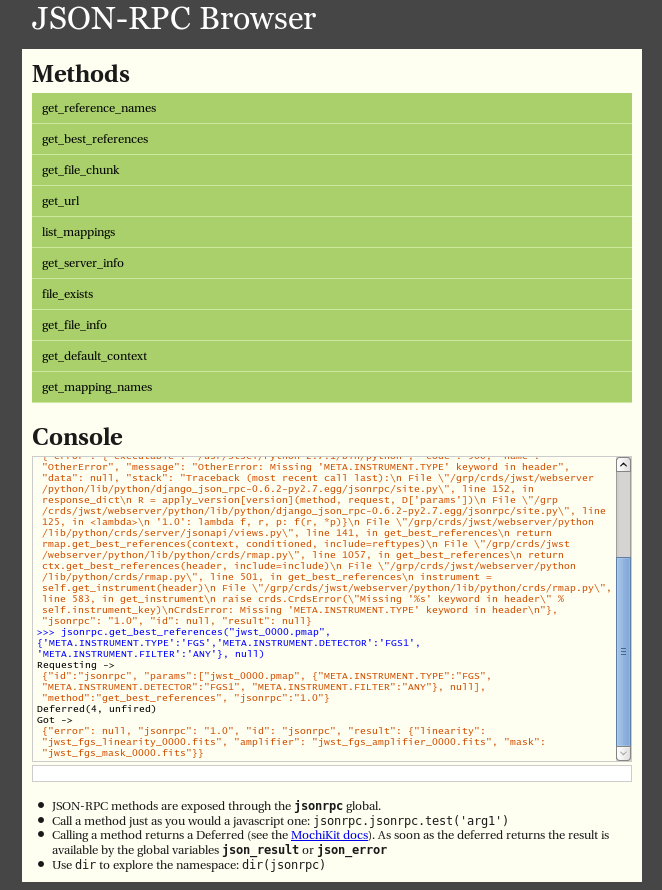
\includegraphics{web_jsonrpc_browse.png}}
\end{figure}

An example dialog for get\_best\_references from the CRDS jsonrpc demo page is
shown here with FITS parkey names:

\begin{Verbatim}[commandchars=\\\{\}]
\PYG{g+gp}{\PYGZgt{}\PYGZgt{}\PYGZgt{} }\PYG{n}{jsonrpc}\PYG{o}{.}\PYG{n}{get\PYGZus{}best\PYGZus{}references}\PYG{p}{(}\PYG{l+s}{\PYGZdq{}}\PYG{l+s}{jwst\PYGZus{}0000.pmap}\PYG{l+s}{\PYGZdq{}}\PYG{p}{,} \PYG{p}{\PYGZob{}}\PYG{l+s}{\PYGZsq{}}\PYG{l+s}{INSTRUME}\PYG{l+s}{\PYGZsq{}}\PYG{p}{:}\PYG{l+s}{\PYGZsq{}}\PYG{l+s}{FGS}\PYG{l+s}{\PYGZsq{}}\PYG{p}{,}\PYG{l+s}{\PYGZsq{}}\PYG{l+s}{DETECTOR}\PYG{l+s}{\PYGZsq{}}\PYG{p}{:}\PYG{l+s}{\PYGZsq{}}\PYG{l+s}{FGS1}\PYG{l+s}{\PYGZsq{}}\PYG{p}{,} \PYG{l+s}{\PYGZsq{}}\PYG{l+s}{FILTER}\PYG{l+s}{\PYGZsq{}}\PYG{p}{:}\PYG{l+s}{\PYGZsq{}}\PYG{l+s}{ANY}\PYG{l+s}{\PYGZsq{}}\PYG{p}{\PYGZcb{}}\PYG{p}{,} \PYG{n}{null}\PYG{p}{)}
\PYG{g+go}{Requesting \PYGZhy{}\PYGZgt{}}
\PYG{g+go}{\PYGZob{}\PYGZdq{}id\PYGZdq{}:\PYGZdq{}jsonrpc\PYGZdq{}, \PYGZdq{}params\PYGZdq{}:[\PYGZdq{}jwst\PYGZus{}0000.pmap\PYGZdq{}, \PYGZob{}\PYGZdq{}INSTRUME\PYGZdq{}:\PYGZdq{}FGS\PYGZdq{}, \PYGZdq{}DETECTOR\PYGZdq{}:\PYGZdq{}FGS1\PYGZdq{}, \PYGZdq{}FILTER\PYGZdq{}:\PYGZdq{}ANY\PYGZdq{}\PYGZcb{}, null], \PYGZdq{}method\PYGZdq{}:\PYGZdq{}get\PYGZus{}best\PYGZus{}references\PYGZdq{}, \PYGZdq{}jsonrpc\PYGZdq{}:\PYGZdq{}1.0\PYGZdq{}\PYGZcb{}}
\PYG{g+go}{Deferred(12, unfired)}
\PYG{g+go}{Got \PYGZhy{}\PYGZgt{}}
\PYG{g+go}{\PYGZob{}\PYGZdq{}error\PYGZdq{}: null, \PYGZdq{}jsonrpc\PYGZdq{}: \PYGZdq{}1.0\PYGZdq{}, \PYGZdq{}id\PYGZdq{}: \PYGZdq{}jsonrpc\PYGZdq{}, \PYGZdq{}result\PYGZdq{}: \PYGZob{}\PYGZdq{}linearity\PYGZdq{}: \PYGZdq{}jwst\PYGZus{}fgs\PYGZus{}linearity\PYGZus{}0000.fits\PYGZdq{}, \PYGZdq{}amplifier\PYGZdq{}: \PYGZdq{}jwst\PYGZus{}fgs\PYGZus{}amplifier\PYGZus{}0000.fits\PYGZdq{}, \PYGZdq{}mask\PYGZdq{}: \PYGZdq{}jwst\PYGZus{}fgs\PYGZus{}mask\PYGZus{}0000.fits\PYGZdq{}\PYGZcb{}\PYGZcb{}}
\end{Verbatim}

And the same query is here with JWST data model parkey names:

\begin{Verbatim}[commandchars=\\\{\}]
\PYG{g+gp}{\PYGZgt{}\PYGZgt{}\PYGZgt{} }\PYG{n}{jsonrpc}\PYG{o}{.}\PYG{n}{get\PYGZus{}best\PYGZus{}references}\PYG{p}{(}\PYG{l+s}{\PYGZdq{}}\PYG{l+s}{jwst\PYGZus{}0000.pmap}\PYG{l+s}{\PYGZdq{}}\PYG{p}{,} \PYG{p}{\PYGZob{}}\PYG{l+s}{\PYGZsq{}}\PYG{l+s}{META.INSTRUMENT.TYPE}\PYG{l+s}{\PYGZsq{}}\PYG{p}{:}\PYG{l+s}{\PYGZsq{}}\PYG{l+s}{FGS}\PYG{l+s}{\PYGZsq{}}\PYG{p}{,}\PYG{l+s}{\PYGZsq{}}\PYG{l+s}{META.INSTRUMENT.DETECTOR}\PYG{l+s}{\PYGZsq{}}\PYG{p}{:}\PYG{l+s}{\PYGZsq{}}\PYG{l+s}{FGS1}\PYG{l+s}{\PYGZsq{}}\PYG{p}{,} \PYG{l+s}{\PYGZsq{}}\PYG{l+s}{META.INSTRUMENT.FILTER}\PYG{l+s}{\PYGZsq{}}\PYG{p}{:}\PYG{l+s}{\PYGZsq{}}\PYG{l+s}{ANY}\PYG{l+s}{\PYGZsq{}}\PYG{p}{\PYGZcb{}}\PYG{p}{,} \PYG{n}{null}\PYG{p}{)}
\PYG{g+go}{Requesting \PYGZhy{}\PYGZgt{}}
\PYG{g+go}{\PYGZob{}\PYGZdq{}id\PYGZdq{}:\PYGZdq{}jsonrpc\PYGZdq{}, \PYGZdq{}params\PYGZdq{}:[\PYGZdq{}jwst\PYGZus{}0000.pmap\PYGZdq{}, \PYGZob{}\PYGZdq{}META.INSTRUMENT.TYPE\PYGZdq{}:\PYGZdq{}FGS\PYGZdq{}, \PYGZdq{}META.INSTRUMENT.DETECTOR\PYGZdq{}:\PYGZdq{}FGS1\PYGZdq{}, \PYGZdq{}META.INSTRUMENT.FILTER\PYGZdq{}:\PYGZdq{}ANY\PYGZdq{}\PYGZcb{}, null], \PYGZdq{}method\PYGZdq{}:\PYGZdq{}get\PYGZus{}best\PYGZus{}references\PYGZdq{}, \PYGZdq{}jsonrpc\PYGZdq{}:\PYGZdq{}1.0\PYGZdq{}\PYGZcb{}}
\PYG{g+go}{Deferred(14, unfired)}
\PYG{g+go}{Got \PYGZhy{}\PYGZgt{}}
\PYG{g+go}{\PYGZob{}\PYGZdq{}error\PYGZdq{}: null, \PYGZdq{}jsonrpc\PYGZdq{}: \PYGZdq{}1.0\PYGZdq{}, \PYGZdq{}id\PYGZdq{}: \PYGZdq{}jsonrpc\PYGZdq{}, \PYGZdq{}result\PYGZdq{}: \PYGZob{}\PYGZdq{}linearity\PYGZdq{}: \PYGZdq{}jwst\PYGZus{}fgs\PYGZus{}linearity\PYGZus{}0000.fits\PYGZdq{}, \PYGZdq{}amplifier\PYGZdq{}: \PYGZdq{}jwst\PYGZus{}fgs\PYGZus{}amplifier\PYGZus{}0000.fits\PYGZdq{}, \PYGZdq{}mask\PYGZdq{}: \PYGZdq{}jwst\PYGZus{}fgs\PYGZus{}mask\PYGZus{}0000.fits\PYGZdq{}\PYGZcb{}\PYGZcb{}}
\end{Verbatim}

\textbf{NOTE:} An apparent bug in the demo interpreter makes it impossible to pass
the get\_best\_references \emph{reftypes} parameter as an array of strings.   In the
current demo reftypes can only be specified as null.


\chapter{CRDS Database Access}
\label{database:crds-database-access}\label{database::doc}

\section{JSON RPC Access}
\label{database:json-rpc-access}
CRDS supports JSON RPC access to the CRDS catalog via the crds.client API.


\subsection{Metadata for a single file}
\label{database:metadata-for-a-single-file}
The JSON RPC call get\_file\_info() will return the avalailble info for a single reference
or mapping file from the specified observatory:

\begin{Verbatim}[commandchars=\\\{\}]
def get\PYGZus{}file\PYGZus{}info(observatory, filename):
     \PYGZdq{}\PYGZdq{}\PYGZdq{}Return a dictionary of CRDS information about {}`filename{}`.\PYGZdq{}\PYGZdq{}\PYGZdq{}

 \PYGZgt{}\PYGZgt{}\PYGZgt{} from crds.client import api

 \PYGZgt{}\PYGZgt{}\PYGZgt{} api.get\PYGZus{}file\PYGZus{}info(\PYGZdq{}hst\PYGZdq{}, file=\PYGZdq{}lcb12060j\PYGZus{}drk.fits\PYGZdq{})
 \PYGZob{}\PYGZsq{}activation\PYGZus{}date\PYGZsq{}: \PYGZsq{}2001\PYGZhy{}12\PYGZhy{}14 20:47:00\PYGZsq{},
  \PYGZsq{}blacklisted\PYGZsq{}: \PYGZsq{}false\PYGZsq{},
  \PYGZsq{}change\PYGZus{}level\PYGZsq{}: \PYGZsq{}severe\PYGZsq{},
  \PYGZsq{}delivery\PYGZus{}date\PYGZsq{}: \PYGZsq{}2013\PYGZhy{}07\PYGZhy{}10 11:26:23\PYGZsq{},
  \PYGZsq{}derived\PYGZus{}from\PYGZsq{}: \PYGZsq{}none\PYGZsq{},
  \PYGZsq{}filekind\PYGZsq{}: \PYGZsq{}darkfile\PYGZsq{},
  \PYGZsq{}instrument\PYGZsq{}: \PYGZsq{}acs\PYGZsq{},
  \PYGZsq{}name\PYGZsq{}: \PYGZsq{}lcb12060j\PYGZus{}drk.fits\PYGZsq{},
  \PYGZsq{}observatory\PYGZsq{}: \PYGZsq{}hst\PYGZsq{},
  \PYGZsq{}pedigree\PYGZsq{}: \PYGZsq{}ground\PYGZsq{},
  \PYGZsq{}rejected\PYGZsq{}: \PYGZsq{}false\PYGZsq{},
  \PYGZsq{}sha1sum\PYGZsq{}: \PYGZsq{}56cfd1107bda5d82cb49a301a50edb45cb64ded6\PYGZsq{},
  \PYGZsq{}size\PYGZsq{}: \PYGZsq{}10549440\PYGZsq{},
  \PYGZsq{}state\PYGZsq{}: \PYGZsq{}operational\PYGZsq{},
  \PYGZsq{}type\PYGZsq{}: \PYGZsq{}reference\PYGZsq{},
  \PYGZsq{}useafter\PYGZus{}date\PYGZsq{}: \PYGZsq{}1992\PYGZhy{}01\PYGZhy{}01 00:00:00\PYGZsq{}\PYGZcb{}
\end{Verbatim}


\subsection{Metadata for several / all files}
\label{database:metadata-for-several-all-files}
The JSON RPC call get\_file\_info\_map() will return the info for multiple (or all) files
and the specified (or all) fields as a dictionary of dictionaries mapping filename onto info:

\begin{Verbatim}[commandchars=\\\{\}]
def get\PYGZus{}file\PYGZus{}info\PYGZus{}map(observatory, files=None, fields=None):
    \PYGZdq{}\PYGZdq{}\PYGZdq{}Return the info \PYGZob{} filename : \PYGZob{} info \PYGZcb{} \PYGZcb{} on {}`files{}` of {}`observatory{}`.
    {}`fields{}` can be used to limit info returned to specified keys.
    \PYGZdq{}\PYGZdq{}\PYGZdq{}

\PYGZpc{} setenv CRDS\PYGZus{}SERVER\PYGZus{}URL https://hst\PYGZhy{}crds.stsci.edu

\PYGZgt{}\PYGZgt{}\PYGZgt{} from crds.client import api

\PYGZgt{}\PYGZgt{}\PYGZgt{} api.get\PYGZus{}file\PYGZus{}info\PYGZus{}map(\PYGZdq{}hst\PYGZdq{}, [\PYGZdq{}lcb12060j\PYGZus{}drk.fits\PYGZdq{}, \PYGZdq{}n3o1022fj\PYGZus{}drk.fits\PYGZdq{}], fields=[\PYGZdq{}state\PYGZdq{},\PYGZdq{}size\PYGZdq{},\PYGZdq{}sha1sum\PYGZdq{}])
\PYGZob{}\PYGZsq{}lcb12060j\PYGZus{}drk.fits\PYGZsq{}: \PYGZob{}\PYGZsq{}sha1sum\PYGZsq{}: \PYGZsq{}56cfd1107bda5d82cb49a301a50edb45cb64ded6\PYGZsq{},
  \PYGZsq{}size\PYGZsq{}: \PYGZsq{}10549440\PYGZsq{},
  \PYGZsq{}state\PYGZsq{}: \PYGZsq{}operational\PYGZsq{}\PYGZcb{},
 \PYGZsq{}n3o1022fj\PYGZus{}drk.fits\PYGZsq{}: \PYGZob{}\PYGZsq{}sha1sum\PYGZsq{}: \PYGZsq{}cecf11300015df8f39913b638138d8c67de77a02\PYGZsq{},
  \PYGZsq{}size\PYGZsq{}: \PYGZsq{}10526400\PYGZsq{},
  \PYGZsq{}state\PYGZsq{}: \PYGZsq{}operational\PYGZsq{}\PYGZcb{}\PYGZcb{}
\end{Verbatim}

If files is specified as \emph{None},  info on all files is returned.

If fields are specified as \emph{None},  info on all available fields is returned.


\section{Download CRDS catalog for SQLite queries}
\label{database:download-crds-catalog-for-sqlite-queries}
The CRDS catalog stores metadata about references not captured in the .rmap files.   It also contains
the history of CRDS context use,  the effective dates at which particular contexts where operational in
the pipeline.

You can download a SQLite-3 snapshot of the CRDS catalog like this:

\begin{Verbatim}[commandchars=\\\{\}]
\PYGZpc{} setenv CRDS\PYGZus{}SERVER\PYGZus{}URL https://hst\PYGZhy{}crds.stsci.edu
\PYGZpc{} setenv CRDS\PYGZus{}PATH /home/jmiller/crds\PYGZus{}cache
\PYGZpc{} python \PYGZhy{}m crds.sync \PYGZhy{}\PYGZhy{}fetch\PYGZhy{}sqlite\PYGZhy{}db
CRDS  : INFO     SQLite database file downloaded to: /home/jmiller/crds\PYGZus{}cache/config/hst/crds\PYGZus{}db.sqlite3
\end{Verbatim}

will snapshot the current CRDS catalog on the CRDS server and download it to your local CRDS cache as a
SQLite3 database file.  The SQLite database can typically be accessed like this:

\begin{Verbatim}[commandchars=\\\{\}]
\PYGZpc{} sqlite3 /home/jmiller/crds\PYGZus{}cache\PYGZus{}dev/config/hst/crds\PYGZus{}db.sqlite3

sqlite\PYGZgt{} .tables
crds\PYGZus{}hst\PYGZus{}catalog       crds\PYGZus{}hst\PYGZus{}context\PYGZus{}history

sqlite\PYGZgt{} .mode tabs
sqlite\PYGZgt{} .headers on
sqlite\PYGZgt{} select * from crds\PYGZus{}hst\PYGZus{}context\PYGZus{}history where state=\PYGZdq{}operational\PYGZdq{} limit 1;
id    name    start\PYGZus{}date        context     state          description
2        2013\PYGZhy{}07\PYGZhy{}02 15:44:53    hst.pmap    operational    set by system
\PYGZbs{}.\PYGZbs{}.\PYGZbs{}.
\end{Verbatim}

The CRDS catalog contains the following meta-data:

\begin{tabulary}{\linewidth}{|L|L|L|}
\hline
\textsf{\relax 
Catalog Fields
} & \textsf{\relax 
type
} & \textsf{\relax 
description
}\\
\hline
name
 & 
str
 & 
CRDS filename
\\

uploaded\_as
 & 
str
 & 
Name of file at time of upload / generation
\\

state
 & 
str
 & 
uploaded, delivered, submitted, archiving, archived, archiving-failed, bad
\\

blacklisted
 & 
bool/int
 & 
True/1 == this mapping,  and all mappings referring to it, are invalid.
\\

rejected
 & 
bool/int
 & 
True/1 == this file is considered scientifically invalid
\\

replaced\_by\_filename
 & 
str
 & 
Succeeding reference file in chain of contexts.  Weakly defined.
\\

instrument
 & 
str
 & 
instrument name file applies to
\\

filekind
 & 
str
 & 
reference type. For HST,  also keyword name for dataset headers
\\

type
 & 
str
 & 
reference or mapping
\\

description
 & 
str
 & 
description given at time of delivery
\\

comment
 & 
str
 & 
COMMENT from reference file
\\

aperture
 & 
str
 & 
APERTURE from reference file
\\

derived\_from
 & 
str
 & 
Name of mapping this one was derived from
\\

sha1sum
 & 
str
 & 
sha1sum of file to verify file integrity
\\

size
 & 
int
 & 
length of file in bytes
\\

creator\_name
 & 
str
 & 
author of reference or mapping file
\\

deliverer\_user
 & 
str
 & 
person who submitted the reference or mapping to CRDS
\\

deliverer\_email
 & 
str
 & 
e-mail of person who submitted reference
\\
\hline\end{tabulary}


\emph{NOTE:} Reference file assignment criteria are encoded in the CRDS rules / mappings and displayed as tables on
the web site context display.   See also crds.matches for information on displaying matching criteria based on rmaps
at the command line.



\renewcommand{\indexname}{Index}
\printindex
\end{document}
